% !TEX root = C:\Users\isabe\Documents\Bachelor_thesis_template___UC3M___IEEE_Style__1_\main.tex
%----------
%   WARNING
%----------

% This Guide contains Library recommendations based mainly on APA and IEEE styles, but you must always follow the guidelines of your TFG Tutor and the TFG regulations for your degree.

% THIS TEMPLATE IS BASED ON THE IEEE STYLE


%----------
% DOCUMENT SETTINGS
%----------

\documentclass[12pt]{report} % font: 12pt

% Tablas
\usepackage{booktabs}        % reglas tipográficas (top/mid/bottom)
\usepackage{comment}
\usepackage{tabularx}        % columna X para ancho automático
\usepackage[table]{xcolor}   % colores en tablas
\rowcolors{2}{gray!15}{white}% filas alternadas (opcional)
\usepackage{longtable}
\usepackage{array} % para p{..}
\usepackage{enumitem} % opciones de espaciado en itemize/enumerate
\usepackage{placeins} % barreras para evitar que flotantes salten entre secciones
\usepackage{multirow}
\usepackage{amssymb} % Para el checkmark
\usepackage{rotating} % Para rotar los encabezados si es necesario
\usepackage{graphicx}
\usepackage{adjustbox}
\usepackage{caption}      % Configuración de captions para tablas y figuras

% margins: 2.5 cm top and bottom; 3 cm left and right
\usepackage[
a4paper,
vmargin=2.5cm,
hmargin=3cm
]{geometry}

% Paragraph Spacing and Line Spacing: Narrow (6 pt / 1.15 spacing) or Moderate (6 pt / 1.5 spacing)
\renewcommand{\baselinestretch}{1.15}
\parskip=6pt
% Remove paragraph indentation throughout the document
\setlength{\parindent}{0pt}

% Color settings for cover and code listings
\usepackage[table]{xcolor}
\definecolor{azulUC3M}{RGB}{0,0,102}
\definecolor{gray97}{gray}{.97}
\definecolor{gray75}{gray}{.75}
\definecolor{gray45}{gray}{.45}

% PDF/A -- Important for its inclusion in e-Archive. PDF/A is the optimal format for preservation and for the generation of metadata: http://uc3m.libguides.com/ld.php?content_id=31389625.

% In the template we include the file OUTPUT.XMPDATA. You can download that file and include the metadata that will be incorporated into the PDF file when you compile the memoria.tex file. Then upload it back to your project.
\usepackage[a-1b]{pdfx}

% LINKS
\usepackage{hyperref}
\hypersetup{colorlinks=true,
	linkcolor=black, % links to parts of the document (e.g. index) in black
	citecolor=black, % citation links in black
	urlcolor=blue} % links to resources outside the document in blue

% MATH EXPRESSIONS
\usepackage{amsmath,amssymb,amsfonts,amsthm}

% Character encoding
\usepackage{txfonts}
\usepackage[T1]{fontenc}
\usepackage[utf8]{inputenc}

% Improve line breaking and reduce unwanted hyphenation
\usepackage{microtype}
% Discourage hyphenation and avoid breaks that leave very short fragments
\hyphenpenalty=5000
\exhyphenpenalty=5000
\lefthyphenmin=3
\righthyphenmin=3

% Spanish settings
\usepackage[spanish,english]{babel}
\usepackage[babel, spanish=spanish]{csquotes}
\addto\captionsspanish{%
	\renewcommand{\contentsname}{Índice}%
	\renewcommand{\listfigurename}{Índice de figuras}%
	\renewcommand{\listtablename}{Lista de tablas}%
	\renewcommand{\bibname}{Bibliografía}%
}
\addto\captionsenglish{%
	\renewcommand{\contentsname}{Índice}%
	\renewcommand{\listfigurename}{Índice de figuras}%
	\renewcommand{\listtablename}{Índice de tablas}%
}
\AtBeginEnvironment{quote}{\small}

% Footer settings
\usepackage{fancyhdr}
\pagestyle{fancy}
\fancyhf{}
\renewcommand{\headrulewidth}{0pt}
\rfoot{\thepage}
\fancypagestyle{plain}{\pagestyle{fancy}}

% DESIGN OF THE TITLES of the parts of the work (chapters and epigraphs or sub-chapters)
\usepackage{titlesec}
\usepackage{titletoc}
\titleformat{\chapter}[block]
{\large\bfseries\filcenter}
{\thechapter.}
{5pt}
{\MakeUppercase}
{}
\titlespacing{\chapter}{0pt}{0pt}{*3}
\titlecontents{chapter}
[0pt]
{}
{\contentsmargin{0pt}\thecontentslabel.\enspace\uppercase}
{\contentsmargin{0pt}\uppercase}
{\titlerule*[.7pc]{.}\contentspage}

\titleformat{\section}
{\bfseries}
{\thesection.}
{5pt}
{}
\titlecontents{section}
[5pt]
{}
{\contentsmargin{0pt}\thecontentslabel.\enspace}
{\contentsmargin{0pt}}
{\titlerule*[.7pc]{.}\contentspage}

\titleformat{\subsection}
{\normalsize\bfseries}
{\thesubsection.}
{5pt}
{}
\titlecontents{subsection}
[10pt]
{}
{\contentsmargin{0pt}
	\thecontentslabel.\enspace}
{\contentsmargin{0pt}}
{\titlerule*[.7pc]{.}\contentspage}


% Tables and figures settings
\usepackage{multirow} % combine cells
\usepackage{caption} % customize the title of tables and figures
\usepackage{floatrow} % we use this package and its \ ttabbox and \ ffigbox macros to align the table and figure names according to the defined style.
\usepackage{float} % para usar posicionamiento [H] en figuras
\usepackage{array} % with this package we can define in the following line a new type of column for tables: custom width and centered content
\newcolumntype{P}[1]{>{\centering\arraybackslash}m{#1}}
\DeclareCaptionFormat{upper}{#1#2\uppercase{#3}\par}
\usepackage{graphicx}
\graphicspath{{imagenes/}} % Images folder

% Table layout for engineering
\captionsetup*[table]{
	%format=upper,
	name=Tabla,
	justification=centering,
	singlelinecheck=false,
	labelsep=period,
	width=.75\linewidth,
	labelfont=small,
	font=small
}

\captionsetup{font=small, textfont=it, labelfont=it, margin=10pt}

% Figures layout for engineering
\captionsetup[figure]{
	format=hang,
	name=Fig.,
	singlelinecheck=off,
	labelsep=period,
	labelfont=small,
	font=small,
	justification=centering
}

% FOOTNOTES
\usepackage{chngcntr} % continuous numbering of footnotes
\counterwithout{footnote}{chapter}

% CODE LISTINGS
% support and styling for listings. More information in  https://es.wikibooks.org/wiki/Manual_de_LaTeX/Listados_de_código/Listados_con_listings
\usepackage{listings}

% Custom listing
\lstdefinestyle{estilo}{ frame=Ltb,
	framerule=0pt,
	aboveskip=0.5cm,
	framextopmargin=3pt,
	framexbottommargin=3pt,
	framexleftmargin=0.4cm,
	framesep=0pt,
	rulesep=.4pt,
	backgroundcolor=\color{gray97},
	rulesepcolor=\color{black},
	%
	basicstyle=\ttfamily\footnotesize,
	keywordstyle=\bfseries,
	stringstyle=\ttfamily,
	showstringspaces = false,
	commentstyle=\color{gray45},
	%
	numbers=left,
	numbersep=15pt,
	numberstyle=\tiny,
	numberfirstline = false,
	breaklines=true,
	xleftmargin=\parindent
}

\captionsetup*[lstlisting]{font=small, labelsep=period}

\lstset{style=estilo}
\renewcommand{\lstlistingname}{\uppercase{Código}}


% REFERENCES

% IEEE bibliography setup
\usepackage[backend=biber, style=ieee, isbn=false,sortcites, maxbibnames=6, minbibnames=1]{biblatex} % Setting for IEEE citation style, recommended for engineering. "maxbibnames" indicates that from 6 authors truncate the list in the first one (minbibnames) and add "et al." as used in the IEEE style.

\addbibresource{referencias.bib} % The references.bib file in which the bibliography used should be


%-------------
%	DOCUMENT
%-------------

\begin{document}
\pagenumbering{roman} % Roman numerals are used in the numbering of the pages preceding the body of the work.

%----------
%	COVER
%----------
\begin{titlepage}
	\begin{sffamily}
	\color{azulUC3M}
	\begin{center}
		\begin{figure}[H] % UC3M Logo
			\makebox[\textwidth][c]{
\includegraphics[width=16cm]{logo_UC3M.png}}
		\end{figure}
		\vspace{2.5cm}
		\begin{Large}
			Grado en Ingeniería Informática.\\
			 2025-2026\\ % Academic year
			\vspace{2cm}
			\textsl{Trabajo de Fin de Grado}
			\bigskip

		\end{Large}
		 	{\Huge ``Plataforma Colaborativa para el Intercambio y Corrección Lingüística''}\\
		 	\vspace*{0.5cm}
	 		\rule{10.5cm}{0.1mm}\\
			\vspace*{0.9cm}
			{\LARGE Mª Isabel Hernández Barrio}\\
			\vspace*{1cm}
		\begin{Large}
			Jesús Hernando Corrochano\\
			Madrid, junio de 2026\\
		\end{Large}
	\end{center}
	\vfill
	\color{black}
	% IF OUR WORK IS TO BE PUBLISHED UNDER A CREATIVE COMMONS LICENSE, INCLUDE THESE LINES. IS THE RECOMMENDED OPTION.
	
\includegraphics[width=4.2cm]{creativecommons.png}\\ % Creative Commons Logo
    This work is licensed under Creative Commons \textbf{Attribution – Non Commercial – Non Derivatives}
	\end{sffamily}
\end{titlepage}

\newpage % blank page
\thispagestyle{empty}
\mbox{}

%----------
%	ABSTRACT AND KEYWORDS
%----------
\begin{abstract}
\thispagestyle{plain}
\setcounter{page}{3}

	% Write your abstract
	Nowadays, the digital transformation of education and language learning has become essential for global communication and international activity. In this context, the creation of a specialized web application for language exchange through written correspondence is presented as an innovative solution to bridge the gap between theoretical knowledge and practical, collaborative learning.

	The aim of this Final Degree Project is to design and develop a web platform, named Letterex, that facilitates language exchange between users worldwide. The tool seeks to provide an efficient and interactive environment where users can practice writing in foreign languages and receive peer-to-peer corrections. Additionally, the application includes a personal space for users to manage their profiles and build a social network based on shared learning interests.

	The process of designing and developing this application involved a detailed analysis of the specific needs of language learners, as well as the implementation of a modern metodology and tech stack. Built using the MERN stack (MongoDB, Express, React, and Node.js), the platform incorporates features such as a secure authentication system via JWT, a module for creating and organizing letters into diaries, a shared correction interface, and a social recommendation algorithm based on language affinity.

	To sum up, this project aims to offer a technological solution tailored to the requirements of modern language learners, optimizing the writing and correcting process and the improvement of linguistic skills through an active and supportive community.

	\textbf{Keywords:} Language exchange, Web development, MERN stack, Peer-to-peer correction, MongoDB, REST API.

	\vfill
\end{abstract}
	\newpage % Blank page
	\thispagestyle{empty}
	\mbox{}


%----------
%	Dedication
%----------
\chapter*{Agradecimientos}
Gracias a mi familia, por su apoyo incondicional a lo largo de mis estudios, ayudándome en cada caída y celebrando cada logro.

Gracias a mis amigos, en especial Luis, David y Viku, por hacer de estos años universitarios una aventura llena de risas, viajes y triángulos de chocolate.

Gracias a mis amigos del Erasmus por inspirar este proyecto, a mi tutor Jesús por acompañarme en su realización, y a mi pareja Miriam y su amiga Ana por revisar las faltas de ortografía.
\setcounter{page}{5}

	% Write here


	\vfill

	\newpage % blank page
	\thispagestyle{empty}
	\mbox{}


%----------
%	TOC
%----------

%--
% TOC
%-
\tableofcontents
\thispagestyle{fancy}

\newpage % blank page
\thispagestyle{empty}
\mbox{}

%--
% List of figures. If they are not included, comment the following lines
%-
\listoffigures
\thispagestyle{fancy}

\newpage % blank page
\thispagestyle{empty}
\mbox{}

%--
% List of tables. If they are not included, comment the following lines
%-
\listoftables
\thispagestyle{fancy}

\newpage % blankpage
\thispagestyle{empty}
\mbox{}

\chapter*{Lista de abreviaturas}
\addcontentsline{toc}{chapter}{Lista de abreviaturas}

\rowcolors{1}{white}{white}
\begin{longtable}{p{2.8cm}p{10.2cm}}
AJAX & Asynchronous JavaScript and XML. \\
API & Application Programming Interface. \\
AKS & Azure Kubernetes Service. \\
AWS & Amazon Web Services. \\
BOE & Boletín Oficial del Estado. \\
BSON & Binary JSON. \\
CORS & Cross-Origin Resource Sharing. \\
CRA & Cyber Resilience Act. \\
CRUD & Create, Read, Update, Delete. \\
CSRF & Cross-Site Request Forgery. \\
CSS & Cascading Style Sheets. \\
DOM & Document Object Model. \\
GCP & Google Cloud Platform. \\
HTML & HyperText Markup Language. \\
HTTP & HyperText Transfer Protocol. \\
JSON & JavaScript Object Notation. \\
JWT & JSON Web Token. \\
LAMP & Linux, Apache, MySQL and PHP. \\
LOPDGDD & Ley Orgánica de Protección de Datos Personales y garantía de los derechos digitales. \\
LSSICE & Ley de Servicios de la Sociedad de la Información y de Comercio Electrónico. \\
MERN & MongoDB, Express, React and Node.js. \\
MIME & Multipurpose Internet Mail Extensions. \\
MVCC & Multi-Version Concurrency Control. \\
NoSQL & Not Only SQL. \\
ODM & Object Document Mapper. \\
ORM & Object Relational Mapper. \\
OTP & One-Time Password. \\
PDF & Portable Document Format. \\
REST & Representational State Transfer. \\
RGPD & Reglamento General de Protección de Datos. \\
SEO & Search Engine Optimization. \\
SMTP & Simple Mail Transfer Protocol. \\
SPA & Single Page Application. \\
SQL & Structured Query Language. \\
SSR & Server-Side Rendering. \\
TFG & Trabajo de Fin de Grado. \\
TTL & Time To Live. \\
URL & Uniform Resource Locator. \\
XML & eXtensible Markup Language. \\
XP & Extreme Programming. \\
XSS & Cross-Site Scripting. \\
\end{longtable}
\rowcolors{2}{gray!15}{white}

\newpage % blank page
\thispagestyle{empty}
\mbox{}


%----------
%	THESIS
%----------
\clearpage
\pagenumbering{arabic} % numbering with Arabic numerals for the rest of the document.


% IMPORTANT: Latex special characters are: # $ % & \ ^ _ { } ~. To avoid mistakes when compiling try writing \ before. For: \ use \textbackslash ; for ^ \textasciitilde and ~ \textasciicircum.

%     Example of figure:
%     \begin{figure}[H]
%     	\ffigbox[\FBwidth] {
%     	\caption[Name as seen in Index]{Figure name}
%     	}
%     	{
\includegraphics[scale=0.6]{imagenes/creativecommons.png}}
%     \end{figure}


%     Example of table:
% \begin{table}[H]
% 	\ttabbox[\FBwidth]
% 	{\caption{Lorem ipsum}}
% 	{\begin{tabular}{|c|P{1.5cm}|c|P{1.5cm}|P{2cm}|c|P{1.5cm}|P{2cm}|}
% 		\hline
% 		\multicolumn{2}{|c|}{\textbf{I}} & \multicolumn{2}{c|}{\textbf{II}} & \multicolumn{3}{c|}{\textbf{III}} & \textbf{IV} \\
% 		\hline
% 		x & y & x & y & x & y & x & y \\
% 		\hline
% 		10.0 & 8.04 & 10.0 & 9.14 & 10.0 & 7.46 & 8.0 & 6.58 \\
% 		\hline
% 		8.0 & 6.95 & 8.0 & 8.14 & 8.0 & 6.77 & 8.0 & 5.76 \\
% 		\hline
% 		13.0 & 7.58 & 13.0 & 8.74 & 13.0 & 12.74 & 8.0 & 7.71 \\
% 		\hline
% 		9.0 & 8.81 & 9.0 & 8.77 & 9.0 & 7.11 & 8.0 & 8.84 \\
% 		\hline
% 		11.0 & 8.33 & 11.0 & 9.26 & 11.0 & 7.81 & 8.0 & 8.47 \\
% 		\hline
% 		14.0 & 9.96 & 14.0 & 8.10 & 14.0 & 8.84 & 8.0 & 7.04 \\
% 		\hline
% 		6.0 & 7.24 & 6.0 & 6.13 & 6.0 & 6.08 & 8.0 & 5.25 \\
% 		\hline
% 		4.0 & 4.26 & 4.0 & 3.10 & 4.0 & 5.39 & 19.0 & 12.50 \\
% 		\hline
% 		12.0 & 10.84 & 12.0 & 9.13 & 12.0 & 8.15 & 8.0 & 5.56 \\
% 		\hline
% 		7.0 & 4.82 & 7.0 & 7.26 & 7.0 & 6.42 & 8.0 & 7.91 \\
% 		\hline
% 		5.0 & 5.68 & 5.0 & 4.74 & 5.0 & 5.73 & 8.0 & 6.89 \\
% 		\hline
% 		\multicolumn{5}{l}{Source: BOE}
% 	\end{tabular}}
% \end{table}


% Start writing here----------------------------------------------------
\input{secciones/introduccion.tex}
\input{secciones/estado_del_arte}
\chapter{Análisis y planificación}

En este capítulo, se lleva a cabo un análisis de las funcionalidades y requerimientos que componen el proyecto, no solo la construcción del software sino el Trabajo de Fin de Grado en su conjunto. Se presentarán las Historias de Usuario, Pruebas de Aceptación y Matriz de Trazabilidad que registran este análisis, seguidas de la planificación que se ha seguido para el desarrollo del proyecto.

\section{Historias de Usuario}

Las Historias de Usuario (HU) son una herramienta básica en la gestión de proyectos mediante metodologías ágiles como SCRUM. Se utilizan para definir las funciones de un sistema desde la perspectiva del usuario final, la forma que las necesidades y funcionalidades que se plantean para el proyecto estén orientadas a aportar valor real al usuario del software. No se debe confundir con los requisitos del sistema, un método más tradicional que suele resultar rígido y técnico en comparación con las Historias de Usuario, las cuales consisten en una explicación breve y directa de cada funcionalidad del sistema.\cite{atlassian_user_stories}

Este enfoque orientado al usuario final se consigue mediante esta fórmula:

    \indent \indent Como \textit{[rol del usuario]}, \\
    \indent \indent quiero \textit{[realizar una acción]}, \\
    \indent \indent para \textit{[obtener un valor o beneficio]}.


Así, se expresa el requerimiento con una descripción concisa, por ejemplo, "Como usuario registrado, quiero recuperar mi contraseña, para poder acceder a mi cuenta en caso de que la olvide". Además, no se trata de un requisito cerrado sino de plantear situaciones para que el cliente y los desarrolladores tengan una conversación sobre las funcionalidades y sus detalles.

\begin{comment}

    Los principios que deben seguir las Historias de Usuario se recogen en el criterio INVEST. Según este criterio, una historia de usuario debe ser:
    \begin{itemize}[itemsep=0pt, parsep=0pt, topsep=3pt, partopsep=0pt]
        \item Independiente: no debe depender de ninguna otra historia de usuario para poder desarrollarse.
        \item Valiosa: debe aportar un beneficio real al usuario, de forma que se invierta esfuerzo en aspectos que verdaderamente satisfagan una necesidad del usuario.
        \item Estimable: debe poder calcularse el esfuerzo que tomará su desarrollo, en este caso mediante puntos de historia, cada uno de los cuales corresponde a 4 horas de trabajo.
        \item Compacta (\textit{Small}): no debe suponer un gran volumen de trabajo sino que debe poder terminarse en unas pocas semanas o días.
        \item Comprobable (\textit{Testable}): las historias deberán ir acompañadas por una confirmación, los criterios para validar que se satisface el objetivo planteado en cada una. En este caso se hará en forma de Pruebas de Aceptación, presentadas en la siguiente sección.
    \end{itemize}
\end{comment}

Cada historia cuenta con: un identificador (HU-XX), que facilitará reconocerlas, cuantificarlas y asociarlas con las Pruebas de Aceptación; una descripción, siguiendo la fórmula presentada anteriormente; su prioridad ('Alta', 'Media' o 'Baja'), que representa la relevancia para el cliente y el orden que ocupará en el desarrollo; la estimación, que cuantifica las horas de trabajo que requiere la compleción de la historia mediante un sistema de puntos en el que 1 punto equivale a 4 horas; las tareas a realizar para satisfacerla; y las Pruebas de Aceptación para validarla.

A continuación, el listado de Historias de Usuario para el proyecto aquí desarrollado separadas en varias secciones: Investigación y Documentación, Gestión de Usuarios, Gestión de Perfiles, Módulo de Correspondencia, Módulo de Correcciones y Funcionalidad Social.

\newcommand{\huPriorityEstimationRow}[2]{%
\textbf{PRIORIDAD} &
\begin{tabularx}{\linewidth}{@{}>{\centering\arraybackslash}X|P{0.18\textwidth}|>{\centering\arraybackslash}X@{}}
#1 & \textbf{ESTIMACIÓN} & #2
\end{tabularx} \\ \hline
}

% --- BLOQUE 1: INVESTIGACIÓN Y DOCUMENTACIÓN ---
\subsection{Investigación y Documentación}

\begin{table}[H]
\centering\small
\begin{tabular}{|P{0.2\textwidth}|P{0.75\textwidth}|}
\hline
\multicolumn{2}{|c|}{\textbf{HU-01}} \\ \hline
\textbf{TÍTULO} & Redacción de apartados introductorios el documento \\ \hline
\huPriorityEstimationRow{Baja}{1}
\textbf{DESCRIPCIÓN} & Como desarrolladora, quiero estructurar e introducir el documento de forma clara, y presentar el marco regulador pertinente. \\ \hline
\textbf{TAREAS} &
    \begin{itemize}[itemsep=0pt, parsep=0pt, topsep=3pt, partopsep=0pt]
        \item Investigar plantillas y normativa de la universidad
        \item Consultar ejemplos de TFG de otros compañeros
        \item Investigar sobre las leyes que componen el marco regulador que incumbe a un proyecto web de este tipo
        \item Redactar los apartados de resumen, dedicación, motivación, objetivos, marco regulador, medios empleados y estructura del documento.
    \end{itemize} \\ \hline
\textbf{PRUEBAS DE ACEPTACIÓN} & PA-02 \\ \hline
\end{tabular}
\caption{HU-01}
\label{tab:HU-01}
\end{table}

\begin{table}[H]
\centering\small
\begin{tabular}{|P{0.2\textwidth}|P{0.75\textwidth}|}
\hline
\multicolumn{2}{|c|}{\textbf{HU-02}} \\ \hline
\textbf{TÍTULO} & Investigación de tecnologías para el desarrollo web \\ \hline
\huPriorityEstimationRow{Alta}{2}
\textbf{DESCRIPCIÓN} & Como desarrolladora, quiero investigar las principales tecnologías para el desarrollo de aplicaciones web para poder hacer una elección sólida y fundada de stack del proyecto \\ \hline
\textbf{TAREAS} &
    \begin{itemize}[itemsep=0pt, parsep=0pt, topsep=3pt, partopsep=0pt]
        \item Investigar tecnologías web para proyectos full-stack
        \item Redactar la primera sección del Estado del Arte
        \item Añadir las referencias bibliográficas necesarias
    \end{itemize}
\\ \hline
\textbf{PRUEBAS DE ACEPTACIÓN} & PA-02 \\ \hline
\end{tabular}
\caption{HU-02}
\label{tab:HU-02}
\end{table}

\begin{table}[H]
\centering\small
\begin{tabular}{|P{0.2\textwidth}|P{0.75\textwidth}|}
\hline
\multicolumn{2}{|c|}{\textbf{HU-03}} \\ \hline
\textbf{TÍTULO} & Investigación de metodologías de desarrollo de software \\ \hline
\huPriorityEstimationRow{Alta}{1}
\textbf{DESCRIPCIÓN} & Como desarrolladora, quiero investigar las principales metodologías para el desarrollo de proyectos de software para trabajar en el proyecto de manera ordenada y planificada \\ \hline
\textbf{TAREAS} &
    \begin{itemize}[itemsep=0pt, parsep=0pt, topsep=3pt, partopsep=0pt]
        \item Investigar metodologías de desarrollo de software
        \item Redactar las segunda sección del Estado del Arte
        \item Añadir las referencias bibliográficas necesarias
    \end{itemize}
\\ \hline
\textbf{PRUEBAS DE ACEPTACIÓN} & PA-02 \\ \hline
\end{tabular}
\caption{HU-03}
\label{tab:HU-03}
\end{table}

\begin{table}[H]
\centering\small
\begin{tabular}{|P{0.2\textwidth}|P{0.75\textwidth}|}
\hline
\multicolumn{2}{|c|}{\textbf{HU-04}} \\ \hline
\textbf{TÍTULO} & Investigación de productos similares en el mercado \\ \hline
\huPriorityEstimationRow{Alta}{1}
\textbf{DESCRIPCIÓN} & Como desarrolladora, quiero investigar sobre otros productos o propuestas similares ya existentes, para un mejor planteamiento del proyecto y de su aporte. \\ \hline
\textbf{TAREAS} &
    \begin{itemize}[itemsep=0pt, parsep=0pt, topsep=3pt, partopsep=0pt]
        \item Investigar propuestas similares a la aquí trabajada
        \item Redactar las tercera sección del Estado del Arte
        \item Añadir las referencias bibliográficas necesarias
        \item Plantear las mejoras y/o puntos novedosos que mi propesta aporta
    \end{itemize}
\\ \hline
\textbf{PRUEBAS DE ACEPTACIÓN} & PA-02 \\ \hline
\end{tabular}
\caption{HU-04}
\label{tab:HU-04}
\end{table}

\begin{table}[H]
\centering\small
\begin{tabular}{|P{0.2\textwidth}|P{0.75\textwidth}|}
\hline
\multicolumn{2}{|c|}{\textbf{HU-05}} \\ \hline
\textbf{TÍTULO} & Análisis de requerimientos y planificación \\ \hline
\huPriorityEstimationRow{Media}{5}
\textbf{DESCRIPCIÓN} & Como desarrolladora, quiero documentar el análisis de los requerimientos del proyecto y dejarlo constatado en forma de las presentes Historias de Usuario, Pruebas de Aceptación y Matriz de trazabilidad; para poder planificar el trabajo mediante la metodología escogida. \\ \hline
\textbf{TAREAS} &
    \begin{itemize}[itemsep=0pt, parsep=0pt, topsep=3pt, partopsep=0pt]
        \item Plantear las necesidades de la aplicación y del documento
        \item Redactar este apartado de "Análisis y Planificación"
        \item Documentar la planificación que se ha seguido y la metodología y
        herramientas que se han utilizado para ello
    \end{itemize}
\\ \hline
\textbf{PRUEBAS DE ACEPTACIÓN} & PA-01, PA-02 \\ \hline
\end{tabular}
\caption{HU-05}
\label{tab:HU-05}
\end{table}

\begin{table}[H]
\centering\small
\begin{tabular}{|P{0.2\textwidth}|P{0.75\textwidth}|}
\hline
\multicolumn{2}{|c|}{\textbf{HU-06}} \\ \hline
\textbf{TÍTULO} & Documentación del prototipado, arquitectura final y modelo económico de la aplicación \\ \hline
\huPriorityEstimationRow{Media}{5}
\textbf{DESCRIPCIÓN} & Como diseñadora, quiero crear prototipos para definir una línea visual representativa de la interfaz de la aplicación, y documentar tanto ese proceso como el producto final de estructura y arquitectura del proyecto de software. \\ \hline
\textbf{TAREAS} &
    \begin{itemize}[itemsep=0pt, parsep=0pt, topsep=3pt, partopsep=0pt]
        \item Crear prototipos de las interfaces de la aplicación e incluirlos en la sección "Análisis y planificación" del documento
        \item Tras desarrollar la aplicación, documentar su estructura y arquitectura en la sección "Arquitectura" del documento
        \item Redacción del apartado de presupuesto del proyecto y marco socio-económico
    \end{itemize}
\\ \hline
\textbf{PRUEBAS DE ACEPTACIÓN} & PA-02 \\ \hline
\end{tabular}
\caption{HU-06}
\label{tab:HU-06}
\end{table}

\begin{table}[H]
\centering\small
\begin{tabular}{|P{0.2\textwidth}|P{0.75\textwidth}|}
\hline
\multicolumn{2}{|c|}{\textbf{HU-07}} \\ \hline
\textbf{TÍTULO} & Plantear conclusiones y líneas de trabajo futuro \\ \hline
\huPriorityEstimationRow{Baja}{1}
\textbf{DESCRIPCIÓN} & Como desarrolladora, al finalizar el grueso del trabajo quiero plantear aspectos del producto final a mejorar en el futuro y conclusiones para cerrar el documento. \\ \hline
\textbf{TAREAS} &
    \begin{itemize}[itemsep=0pt, parsep=0pt, topsep=3pt, partopsep=0pt]
        \item Analizar el producto final para hacer una reflexión de las posibles mejoras a futuro y del recorrido de aprendizaje en la realización de este trabajo
        \item Redactar sección de "Líneas de Trabajo Futuro y Conclusión"
    \end{itemize}
\\ \hline
\textbf{PRUEBAS DE ACEPTACIÓN} & PA-02 \\ \hline
\end{tabular}
\caption{HU-07}
\label{tab:HU-07}
\end{table}

% --- BLOQUE 2: GESTIÓN DE USUARIOS ---
\FloatBarrier
\subsection{Gestión de Usuarios}

\begin{table}[H]
\centering\small
\begin{tabular}{|P{0.2\textwidth}|P{0.75\textwidth}|}
\hline
\multicolumn{2}{|c|}{\textbf{HU-08}} \\ \hline
\textbf{TÍTULO} & Registro e inicio de sesión \\ \hline
\huPriorityEstimationRow{Alta}{5}
\textbf{DESCRIPCIÓN} & Como usuario visitante, quiero registrarme con mis datos y correo electrónico para acceder a las funcionalidades de mi cuenta de forma segura.\\ \hline
\textbf{TAREAS} &
    \begin{itemize}[itemsep=0pt, parsep=0pt, topsep=3pt, partopsep=0pt]
        \item Crear una interfaz con formulario de registro e inicio de sesión
        \item Incluir verificación via email de la identidad del usuario para el registro
        \item Facilitar la entrega de un token de autenticación de usuario para obtener los datos que le correspondan en cada página, poder mantener la sesión abierta, y proteger las rutas privadas de la aplicación
        \item Crear los servicios de registro e inicio de sesión en la API
    \end{itemize}\\ \hline
\textbf{PRUEBAS DE ACEPTACIÓN} & PA-03, PA-04, PA-06, PA-09 \\ \hline
\end{tabular}
\caption{HU-08}
\label{tab:HU-08}
\end{table}

\begin{table}[H]
\centering\small
\begin{tabular}{|P{0.2\textwidth}|P{0.75\textwidth}|}
\hline
\multicolumn{2}{|c|}{\textbf{HU-09}} \\ \hline
\textbf{TÍTULO} & Navegación entre página y Cierre de sesión \\ \hline
\huPriorityEstimationRow{Media}{1}
\textbf{DESCRIPCIÓN} & Como usuario registrado, quiero poder navegar fácilmente entre las páginas de la aplicación y cerrar la sesión iniciada \\ \hline
\textbf{TAREAS} &
    \begin{itemize}[itemsep=0pt, parsep=0pt, topsep=3pt, partopsep=0pt]
        \item Crear un menú desplegable con links a las diferentes páginas y la opción de cerrar la sesión
        \item Asegurarse de que se limpia el token de autenticación al cerrar la sesión
    \end{itemize}
 \\ \hline
\textbf{PRUEBAS DE ACEPTACIÓN} & PA-07, PA-08 \\ \hline
\end{tabular}
\caption{HU-09}
\label{tab:HU-09}
\end{table}

\begin{table}[H]
\centering\small
\begin{tabular}{|P{0.2\textwidth}|P{0.75\textwidth}|}
\hline
\multicolumn{2}{|c|}{\textbf{HU-10}} \\ \hline
\textbf{TÍTULO} & Recuperación de contraseña \\ \hline
\huPriorityEstimationRow{Baja}{1}
\textbf{DESCRIPCIÓN} & Como usuario, quiero poder recuperar mi acceso a la plataforma si olvido la contraseña. \\ \hline
\textbf{TAREAS} &
    \begin{itemize}[itemsep=0pt, parsep=0pt, topsep=3pt, partopsep=0pt]
        \item Crear una interfaz para la recuperación de contraseña y selección de una nueva
        \item Crear un sistema de envío automático de un código de verificación por correo electrónico para la identificación del usuario
    \end{itemize}\\ \hline
\textbf{PRUEBAS DE ACEPTACIÓN} & PA-05 \\ \hline
\end{tabular}
\caption{HU-10}
\label{tab:HU-10}
\end{table}

% --- BLOQUE 3: PERFILES Y GOOGLE DRIVE ---
\FloatBarrier
\subsection{Gestión de Perfiles}

\begin{table}[H]
\centering\small
\begin{tabular}{|P{0.2\textwidth}|P{0.75\textwidth}|}
\hline
\multicolumn{2}{|c|}{\textbf{HU-11}} \\ \hline
\textbf{TÍTULO} & Visualización y Edición de perfil de usuario \\ \hline
\huPriorityEstimationRow{Alta}{5}
\textbf{DESCRIPCIÓN} & Como usuario, quiero editar mis idiomas, biografía, imagen de perfil y país en mi página de perfil, así como mi contraseña. \\ \hline
\textbf{TAREAS} &
    \begin{itemize}[itemsep=0pt, parsep=0pt, topsep=3pt, partopsep=0pt]
        \item Crear una interfaz que muestre los datos de perfil del usuario y que permita editarlos
        \item Crear un componente que permita cargar imágenes a la plataforma
        \item Implementar un mapa que muestre el país del usuario y que le permita editarlo
        \item Añadir la opción de cambiar la contraseña del usuario
        \item Crear un servicio para editar datos de perfil
        \item Crear un servicio para editar la contraseña, reforzando la seguridad pidiendo la contraseña actual, además de la autenticación
    \end{itemize}\\ \hline
\textbf{PRUEBAS DE ACEPTACIÓN} & PA-10, PA-11, PA-12 \\ \hline
\end{tabular}
\caption{HU-11}
\label{tab:HU-11}
\end{table}

\begin{table}[H]
\centering\small
\begin{tabular}{|P{0.2\textwidth}|P{0.75\textwidth}|}
\hline
\multicolumn{2}{|c|}{\textbf{HU-12}} \\ \hline
\textbf{TÍTULO} & Eliminación de cuenta \\ \hline
\huPriorityEstimationRow{Baja}{1}
\textbf{DESCRIPCIÓN} & Como usuario registrado, quiero poder eliminar mi cuenta de forma permanente para que mis datos personales sean borrados del sistema. \\ \hline
\textbf{TAREAS} &
    \begin{itemize}[itemsep=0pt, parsep=0pt, topsep=3pt, partopsep=0pt]
        \item Crear un apartado de configuración en la interfaz de mi perfil de usuario
        \item Implementar un modal en que se pida una doble confirmación de la acción para evitar borrados accidentales
        \item Crear el servicio encargado de la eliminación de los datos del usuario en la base de datos
        \item Asegurar el cierre de sesión automático y la redirección a la página de inicio tras la eliminación
    \end{itemize}\\ \hline
\textbf{PRUEBAS DE ACEPTACIÓN} & PA-13 \\ \hline
\end{tabular}
\caption{HU-12}
\label{tab:HU-12}
\end{table}

\begin{table}[H]
\centering\small
\begin{tabular}{|P{0.2\textwidth}|P{0.75\textwidth}|}
\hline
\multicolumn{2}{|c|}{\textbf{HU-13}} \\ \hline
\textbf{TÍTULO} & Visualización de perfiles de otros usuario \\ \hline
\huPriorityEstimationRow{Media}{1}
\textbf{DESCRIPCIÓN} & Como usuario, quiero ver el perfil de otros para conocer sobre ellos y decidir si quiero agregarlos. \\ \hline
\textbf{TAREAS} &
    \begin{itemize}[itemsep=0pt, parsep=0pt, topsep=3pt, partopsep=0pt]
        \item Modificar la interfaz anterior de perfil de usuario para que sirva como visualizador tanto de perfil propio como de perfil ajeno, restringiendo las funciones de edición si es ajeno
    \end{itemize} \\ \hline
\textbf{PRUEBAS DE ACEPTACIÓN} & PA-14 \\ \hline
\end{tabular}
\caption{HU-13}
\label{tab:HU-13}
\end{table}

% --- BLOQUE 4: CARTAS ---
\FloatBarrier
\subsection{Módulo de Correspondencia}

\begin{table}[H]
\centering\small
\begin{tabular}{|P{0.2\textwidth}|P{0.75\textwidth}|}
\hline
\multicolumn{2}{|c|}{\textbf{HU-14}} \\ \hline
\textbf{TÍTULO} & Creación de cartas \\ \hline
\huPriorityEstimationRow{Alta}{5}
\textbf{DESCRIPCIÓN} & Como usuario, quiero escribir cartas en diferentes idiomas otorgándoles un título, una fecha, una especificación del idioma en que están escritas, su contenido; además de tener la opción de clasificarlas por diario. \\ \hline
\textbf{TAREAS} &
    \begin{itemize}[itemsep=0pt, parsep=0pt, topsep=3pt, partopsep=0pt]
        \item Crear una interfaz que permita la creación de una carta nueva, que cuente con un editores que permitan especificar todos los datos de una carta (título, contenido, fecha, diario, idioma)
        \item Crear la lógica que guarde los datos de una carta en la base de datos
    \end{itemize}\\ \hline
\textbf{PRUEBAS DE ACEPTACIÓN} & PA-15 \\ \hline
\end{tabular}
\caption{HU-14}
\label{tab:HU-14}
\end{table}

\begin{table}[H]
\centering\small
\begin{tabular}{|P{0.2\textwidth}|P{0.75\textwidth}|}
\hline
\multicolumn{2}{|c|}{\textbf{HU-15}} \\ \hline
\textbf{TÍTULO} & Gestión de borradores \\ \hline
\huPriorityEstimationRow{Alta}{2}
\textbf{DESCRIPCIÓN} & Como autor, quiero guardar mi progreso para terminar la carta en otro momento. \\ \hline
\textbf{TAREAS} &
    \begin{itemize}[itemsep=0pt, parsep=0pt, topsep=3pt, partopsep=0pt]
        \item Incluir el la interfaz de creación de carta la opción de guardar la carta
        \item Crear una interfaz que permita acceder a una carta, editarla y guardar los cambios
    \end{itemize}\\ \hline
\textbf{PRUEBAS DE ACEPTACIÓN} & PA-15 \\ \hline
\end{tabular}
\caption{HU-15}
\label{tab:HU-15}
\end{table}


\begin{table}[H]
\centering\small
\begin{tabular}{|P{0.2\textwidth}|P{0.75\textwidth}|}
\hline
\multicolumn{2}{|c|}{\textbf{HU-16}} \\ \hline
\textbf{TÍTULO} & Envío de cartas \\ \hline
\huPriorityEstimationRow{Alta}{2}
\textbf{DESCRIPCIÓN} & Como autor, quiero compartir mis cartas con amigos. \\ \hline
\textbf{TAREAS} &
    \begin{itemize}[itemsep=0pt, parsep=0pt, topsep=3pt, partopsep=0pt]
        \item Incluir en la interfaz de edición de carta la opción de enviarla a amigos
        \item Crear el servicio para compartir una carta con otro usuario
    \end{itemize}\\ \hline
\textbf{PRUEBAS DE ACEPTACIÓN} & PA-16, PA-17 \\ \hline
\end{tabular}
\caption{HU-16}
\label{tab:HU-16}
\end{table}

\begin{table}[H]
\centering\small
\begin{tabular}{|P{0.2\textwidth}|P{0.75\textwidth}|}
\hline
\multicolumn{2}{|c|}{\textbf{HU-17}} \\ \hline
\textbf{TÍTULO} & Listado y filtrado de cartas enviadas \\ \hline
\huPriorityEstimationRow{Alta}{5}
\textbf{DESCRIPCIÓN} & Como usuario, quiero ver la lista de mis cartas, con la opción de aplicar filtros para encontrar cartas determinadas más fácilmente. \\ \hline
\textbf{TAREAS} &
    \begin{itemize}[itemsep=0pt, parsep=0pt, topsep=3pt, partopsep=0pt]
        \item Crear una interfaz que muestre las cartas escritas por el usuario
        \item Añadir barras con herramientas de filtrado por título, idioma o diario
        \item Añadir opción de visualizar la lista ordenada por diarios, y la lista de diarios.
        \item Crear el servicio para acceder al listado de cartas
        \item Implementar paginación y filtrado en este servicio
    \end{itemize}\\ \hline
\textbf{PRUEBAS DE ACEPTACIÓN} & PA-18 \\ \hline
\end{tabular}
\caption{HU-17}
\label{tab:HU-17}
\end{table}

\begin{table}[H]
\centering\small
\begin{tabular}{|P{0.2\textwidth}|P{0.75\textwidth}|}
\hline
\multicolumn{2}{|c|}{\textbf{HU-18}} \\ \hline
\textbf{TÍTULO} & Eliminación lógica de cartas \\ \hline
\huPriorityEstimationRow{Baja}{2}
\textbf{DESCRIPCIÓN} & Como usuario, quiero poder borrar mis cartas sin que desaparezcan del buzón de otros. \\ \hline
\textbf{TAREAS} &
    \begin{itemize}[itemsep=0pt, parsep=0pt, topsep=3pt, partopsep=0pt]
        \item Añadir a la interfaz con la lista de cartas creadas por el usuario la opción de borrar una selección de cartas
        \item Pedir confirmación del usuario antes de realizar el borrado
        \item Crear los servicios encargados del borrado lógico de cartas
    \end{itemize}\\ \hline
\textbf{PRUEBAS DE ACEPTACIÓN} & PA-19, PA-20 \\ \hline
\end{tabular}
\caption{HU-18}
\label{tab:HU-18}
\end{table}


% --- BLOQUE 5: CORRECCIONES ---
\FloatBarrier
\subsection{Módulo de Correcciones}

\begin{table}[H]
\centering\small
\begin{tabular}{|P{0.2\textwidth}|P{0.75\textwidth}|}
\hline
\multicolumn{2}{|c|}{\textbf{HU-19}} \\ \hline
\textbf{TÍTULO} & Listado y filtrado de cartas para corregir \\ \hline
\huPriorityEstimationRow{Alta}{3}
\textbf{DESCRIPCIÓN} & Como revisor, quiero ver qué cartas han compartido conmigo para empezar a corregir, con la opción de aplicar filtros para encontrar cartas determinadas fácilmente, y pudiendo ver claramente cuáles de esas cartas ya han sido corregidas y cuáles no. \\ \hline
\textbf{TAREAS} &
    \begin{itemize}[itemsep=0pt, parsep=0pt, topsep=3pt, partopsep=0pt]
        \item Añadir a la interfaz de cartas creadas, un apartado con la lista de cartas recibidas
        \item Incluir en esta lista una distinción por colores de carta corregida o pendiente
        \item Añadir barras con herramientas de filtrado por título, remitente o si la carta está pendiente de corregir
        \item Crear el servicio para acceder al listado de cartas recibidas
        \item Implementar paginación y filtrado en este servicio
    \end{itemize}\\ \hline
\textbf{PRUEBAS DE ACEPTACIÓN} & PA-21 \\ \hline
\end{tabular}
\caption{HU-19}
\label{tab:HU-19}
\end{table}

\begin{table}[H]
\centering\small
\begin{tabular}{|P{0.2\textwidth}|P{0.75\textwidth}|}
\hline
\multicolumn{2}{|c|}{\textbf{HU-20}} \\ \hline
\textbf{TÍTULO} & Eliminación de cartas recibidas \\ \hline
\huPriorityEstimationRow{Baja}{1}
\textbf{DESCRIPCIÓN} & Como revisor, quiero poder borrar de mi buzón de recibidas aquellas cartas que han sido eliminadas por el usuario que me las envió, en caso de no querer conservar la carta y las correcciones que le he aplicado. \\ \hline
\textbf{TAREAS} &
    \begin{itemize}[itemsep=0pt, parsep=0pt, topsep=3pt, partopsep=0pt]
        \item Añadir a la interfaz con la lista de cartas recibidas la opción de eliminar una carta que ha sido eliminada por su autor
        \item Crear el servicio encargado del borrado físico de cartas (si la carta es eliminada tanto por creador como por remitente, no hay necesidad de mantener el registro en la base de datos)
    \end{itemize}\\ \hline
\textbf{PRUEBAS DE ACEPTACIÓN} & PA-22 \\ \hline
\end{tabular}
\caption{HU-20}
\label{tab:HU-20}
\end{table}


\begin{table}[H]
\centering\small
\begin{tabular}{|P{0.2\textwidth}|P{0.75\textwidth}|}
\hline
\multicolumn{2}{|c|}{\textbf{HU-21}} \\ \hline
\textbf{TÍTULO} & Realización de corrección de texto \\ \hline
\huPriorityEstimationRow{Alta}{4}
\textbf{DESCRIPCIÓN} & Como revisor, quiero añadir correcciones sobre el texto de mi amigo para señalar sus errores u ofrecer sugerencias. \\ \hline
\textbf{TAREAS} &
    \begin{itemize}[itemsep=0pt, parsep=0pt, topsep=3pt, partopsep=0pt]
        \item Crear una interfaz de correción que permita visualizar una carta recibida y añadir correcciones sobre su contenido
        \item Incluir en dicha interfaz la opción de guardar la corrección para editarla más adelante
        \item Crear el servicio para guardas las correcciones y acceder a ellas
    \end{itemize}\\ \hline
\textbf{PRUEBAS DE ACEPTACIÓN} & PA-23 \\ \hline
\end{tabular}
\caption{HU-21}
\label{tab:HU-21}
\end{table}

\begin{table}[H]
\centering\small
\begin{tabular}{|P{0.2\textwidth}|P{0.75\textwidth}|}
\hline
\multicolumn{2}{|c|}{\textbf{HU-22}} \\ \hline
\textbf{TÍTULO} & Añadir comentarios finales a la corrección \\ \hline
\huPriorityEstimationRow{Media}{1}
\textbf{DESCRIPCIÓN} & Como revisor, quiero escribir una nota explicativa al final de mi corrección. \\ \hline
\textbf{TAREAS} &
    \begin{itemize}[itemsep=0pt, parsep=0pt, topsep=3pt, partopsep=0pt]
        \item Incluir en la interfaz de correción un campo para añadir retroalimentación o comentarios finales
        \item Incluir en el servicio de guardado y acceso a cartas corregidas este campo
    \end{itemize}\\ \hline
\textbf{PRUEBAS DE ACEPTACIÓN} & PA-23 \\ \hline
\end{tabular}
\caption{HU-22}
\label{tab:HU-22}
\end{table}

\begin{table}[H]
\centering\small
\begin{tabular}{|P{0.2\textwidth}|P{0.75\textwidth}|}
\hline
\multicolumn{2}{|c|}{\textbf{HU-23}} \\ \hline
\textbf{TÍTULO} & Devolución de la corrección al autor \\ \hline
\huPriorityEstimationRow{Alta}{1}
\textbf{DESCRIPCIÓN} & Como revisor, quiero marcar la corrección como enviada para que mi amigo la vea. \\ \hline
\textbf{TAREAS} &
    \begin{itemize}[itemsep=0pt, parsep=0pt, topsep=3pt, partopsep=0pt]
        \item Añadir en la interfaz de corrección la opción de enviar la correción de vuelta: un botón "Send Back"
        \item Crear el servicio para enviar la carta de vuelta a su autor con las correcciones y comentarios añadidos
    \end{itemize}\\ \hline
\textbf{PRUEBAS DE ACEPTACIÓN} & PA-23 \\ \hline
\end{tabular}
\caption{HU-23}
\label{tab:HU-23}
\end{table}


\begin{table}[H]
\centering\small
\begin{tabular}{|P{0.2\textwidth}|P{0.75\textwidth}|}
\hline
\multicolumn{2}{|c|}{\textbf{HU-24}} \\ \hline
\textbf{TÍTULO} & Visualización de correcciones recibidas \\ \hline
\huPriorityEstimationRow{Alta}{2}
\textbf{DESCRIPCIÓN} & Como remitente, quiero recibir la corrección de la carta que envié a mi amigo una vez este la haya corregido y enviado de vuelta. \\ \hline
\textbf{TAREAS} &
    \begin{itemize}[itemsep=0pt, parsep=0pt, topsep=3pt, partopsep=0pt]
        \item Añadir a las tarjetas de la interfaz de listas de cartas un botón por cada corrección recibida para esa carta.
        \item Crear una página de visualización de corrección, similar a la de corrección pero no editable.
        \item Añadir un link hacia esa página al click del botón mencionado anteriormente.
        \item Crear el servicio para obtener la información de la corrección de una carta.
    \end{itemize}\\ \hline
\textbf{PRUEBAS DE ACEPTACIÓN} & PA-24 \\ \hline
\end{tabular}
\caption{HU-24}
\label{tab:HU-24}
\end{table}

% --- BLOQUE 6: SOCIAL ---
\FloatBarrier
\subsection{Funcionalidad Social}

\begin{table}[H]
\centering\small
\begin{tabular}{|P{0.2\textwidth}|P{0.75\textwidth}|}
\hline
\multicolumn{2}{|c|}{\textbf{HU-25}} \\ \hline
\textbf{TÍTULO} & Listado de usuarios sugeridos \\ \hline
\huPriorityEstimationRow{Alta}{3}
\textbf{DESCRIPCIÓN} & Como usuario, quiero que al plataforma me sugiera usuarios que puedo añadir como amigos basándose en intereses lingüísticos comunes. \\ \hline
\textbf{TAREAS} &
    \begin{itemize}[itemsep=0pt, parsep=0pt, topsep=3pt, partopsep=0pt]
        \item Crear una interfaz que muestra una lista de usuarios sugeridos
        \item Crear el servicio para acceder y crear dicha lista mediante un algoritmo de recomendación personalizado
    \end{itemize}\\ \hline
\textbf{PRUEBAS DE ACEPTACIÓN} & PA-25 \\ \hline
\end{tabular}
\caption{HU-25}
\label{tab:HU-25}
\end{table}

\begin{table}[H]
\centering\small
\begin{tabular}{|P{0.2\textwidth}|P{0.75\textwidth}|}
\hline
\multicolumn{2}{|c|}{\textbf{HU-26}} \\ \hline
\textbf{TÍTULO} & Búsqueda de usuarios por nombre de usuario \\ \hline
\huPriorityEstimationRow{Alta}{1}
\textbf{DESCRIPCIÓN} & Como usuario, quiero buscar personas para agregarlas a mi lista de amigos. \\ \hline
\textbf{TAREAS} &
    \begin{itemize}[itemsep=0pt, parsep=0pt, topsep=3pt, partopsep=0pt]
        \item Incluir en la interfaz de amistades una barra de búsqueda para realizar la tarea
        \item Crear la lógica para obtener una lista de usuarios a partir de una búsqueda
    \end{itemize}\\ \hline
\textbf{PRUEBAS DE ACEPTACIÓN} & PA-26 \\ \hline
\end{tabular}
\caption{HU-26}
\label{tab:HU-26}
\end{table}

\begin{table}[H]
\centering\small
\begin{tabular}{|P{0.2\textwidth}|P{0.75\textwidth}|}
\hline
\multicolumn{2}{|c|}{\textbf{HU-27}} \\ \hline
\textbf{TÍTULO} & Gestión de solicitudes de amistad \\ \hline
\huPriorityEstimationRow{Alta}{2}
\textbf{DESCRIPCIÓN} & Como usuario, quiero solicitar amistad a alguien para intercambiar cartas y correcciones; y rechazar o aceptar las solicitudes de amistad que me lleguen. \\ \hline
\textbf{TAREAS} &
    \begin{itemize}[itemsep=0pt, parsep=0pt, topsep=3pt, partopsep=0pt]
        \item Añadir a las tarjetas de usuarios sugeridos o buscados de la interfaz de amistades un botón para enviar una solicitud de amistad
        \item Crear el servicio para enviar una solicitud de amistad
        \item Añadir un componente de interfaz que muestre la lista de solicitudes de amistad recibidas
        \item Incluir en cada tarjeta de solicitud información básica del usuario que la envió y botones con las opciones de rechazarla o aceptarla
        \item Crear los servicios para rechazar y aceptar solicitudes de amistad
    \end{itemize}\\ \hline
\textbf{PRUEBAS DE ACEPTACIÓN} & PA-27, PA-28 \\ \hline
\end{tabular}
\caption{HU-27}
\label{tab:HU-27}
\end{table}


\begin{table}[H]
\centering\small
\begin{tabular}{|P{0.2\textwidth}|P{0.75\textwidth}|}
\hline
\multicolumn{2}{|c|}{\textbf{HU-28}} \\ \hline
\textbf{TÍTULO} & Visualización y Gestión del Listado de amigos \\ \hline
\huPriorityEstimationRow{Baja}{1}
\textbf{DESCRIPCIÓN} & Como usuario, quiero ver quiénes son mis amigos actuales para saber con quién puedo interactuar, así como eliminar un contacto si ya no es de mi interés intercambiar cartas con él. \\ \hline
\textbf{TAREAS} &
    \begin{itemize}[itemsep=0pt, parsep=0pt, topsep=3pt, partopsep=0pt]
        \item Añadir un componente de interfaz que muestre la lista de amigos del usuario
        \item Crear el servicio para acceder a la lista de amigos del usuario
        \item Añadir un componente de interfaz que permita eliminar un amigo de la lista de contactos
        \item Crear el servicio para eliminar una relación entre usuarios
    \end{itemize}\\ \hline
\textbf{PRUEBAS DE ACEPTACIÓN} & PA-29, PA-30 \\ \hline
\end{tabular}
\caption{HU-28}
\label{tab:HU-28}
\end{table}


\newpage
\section{Pruebas de Aceptación}

En esta sección se detallan los procedimientos de prueba para validar las Historias de Usuario. Cada prueba cuenta con un identificador (PA-XX), un título, las Historias de Usuario que cubre, una descripción, y el procedimiento a seguir para realizarla. No se especifica la compleción de estas ya que todas ellas han sido completadas con éxito. Se encuentran divididas en las mismas secciones que las Historias de Usuario.

% --- PA BLOQUE 1: DOCUMENTACIÓN ---

\subsection{Investigación y Documentación}
\setlength{\tabcolsep}{7pt}

\begin{table}[H]
\centering\small
\begin{tabular}{|P{0.22\textwidth}|P{0.73\textwidth}|}
\hline
\textbf{IDENTIFICADOR} & PA-01 \\ \hline
\textbf{TÍTULO} & Aceptación de la propuesta \\ \hline
\textbf{HU IMPLICADAS} & HU-05 \\ \hline
\textbf{DESCRIPCIÓN} & Obtención de una validación positiva por parte del tutor de las historias de usuario. \\ \hline
\textbf{PROCEDIMIENTO} &
    \begin{enumerate}[itemsep=0pt, parsep=0pt, topsep=3pt, partopsep=0pt]
        \item Redacción de historias de usuario
        \item Validación de estas en una revisión con el tutor
    \end{enumerate}. \\ \hline
\end{tabular}
\caption{PA-01}
\label{tab:PA-01}
\end{table}

\begin{table}[H]
\centering\small
\begin{tabular}{|P{0.22\textwidth}|P{0.73\textwidth}|}
\hline
\textbf{IDENTIFICADOR} & PA-02 \\ \hline
\textbf{TÍTULO} & Aceptación de la estructura y contenido del documento \\ \hline
\textbf{HU IMPLICADAS} & HU-01, HU-02, HU-03, HU-04, HU-05, HU-06, HU-07 \\ \hline
\textbf{DESCRIPCIÓN} & Obtención de una validación positiva por parte del tutor de la estructura planteada en el documento, el esqueleto de las diferentes secciones y su contenido. \\ \hline
\textbf{PROCEDIMIENTO} &
        El tutor valida que la documentación cumple con los requisitos establecidos. \\ \hline
\end{tabular}
\caption{PA-02}
\label{tab:PA-02}
\end{table}

% --- PA BLOQUE 2: USUARIOS ---

\subsection{Gestión de Usuarios}

\begin{table}[H]
\centering\small
\begin{tabular}{|P{0.22\textwidth}|P{0.73\textwidth}|}
\hline
\textbf{IDENTIFICADOR} & PA-03 \\ \hline
\textbf{TÍTULO} & Registro en la plataforma como nuevo usuario \\ \hline
\textbf{HU IMPLICADAS} & HU-08 \\ \hline
\textbf{DESCRIPCIÓN} & Asegurar que un nuevo usuario puede registrarse y que el sistema impide el registro hasta que el correo es verificado. \\ \hline
\textbf{PROCEDIMIENTO} &
        \begin{enumerate}[itemsep=0pt, parsep=0pt, topsep=3pt, partopsep=0pt]
            \item El usuario accede a la URL de la aplicación a través de su navegador.
            \item El usuario selecciona el botón "Register" para iniciar el proceso de registro.
            \item El usuario introduce un nombre de usuario y una contraseña.
            \item El sistema valida los datos introducidos. En caso de que el nombre tenga menos de 5 caracteres o la contraseña menos de 8, se muestra un mensaje de error.
            \item El usuario introduce un correo electrónico para vincular la cuenta.
            \item El sistema envía un código de verificación al correo electrónico proporcionado.
            \item El usuario introduce el código de verificación en la interfaz.
            \item El sistema valida el código. En caso de ser incorrecto, se muestra un mensaje de error.
            \item El usuario selecciona los idiomas que domina. En caso de no seleccionar ninguno, se muestra un mensaje de error.
            \item El usuario selecciona los idiomas que desea aprender. En caso de no seleccionar ninguno, se muestra un mensaje de error.
            \item El sistema muestra un resumen de los datos introducidos, incluyendo la opción de añadir una imagen de perfil.
            \item El usuario, de forma opcional, añade una imagen de perfil y selecciona el botón "All set" para finalizar el registro.
            \item El sistema crea el nuevo usuario con los datos proporcionados y almacena la imagen de perfil en caso de haber sido añadida.
    \end{enumerate}\\ \hline
\end{tabular}
\caption{PA-03}
\label{tab:PA-03}
\end{table}

\begin{table}[H]
\centering\small
\begin{tabular}{|P{0.22\textwidth}|P{0.73\textwidth}|}
\hline
\textbf{IDENTIFICADOR} & PA-04 \\ \hline
\textbf{TÍTULO} & Inicio de sesión en la plataforma \\ \hline
\textbf{HU IMPLICADAS} & HU-08 \\ \hline
\textbf{DESCRIPCIÓN} & Asegurar que un usuario puede acceder a la plataforma introduciendo sus credenciales. \\ \hline
\textbf{PROCEDIMIENTO} &
    \begin{enumerate}[itemsep=0pt, parsep=0pt, topsep=3pt, partopsep=0pt]
        \item El usuario selecciona el botón "Log in" para acceder al formulario de inicio de sesión.
        \item El usuario introduce su nombre de usuario o correo electrónico, junto con su contraseña.
        \item El sistema valida las credenciales introducidas.
        \item En caso de ser correctas, el usuario es redirigido a la página principal. En caso contrario, el sistema muestra un mensaje de error en el formulario.
    \end{enumerate}\\ \hline
\end{tabular}
\caption{PA-04}
\label{tab:PA-04}
\end{table}

\begin{table}[H]
\centering\small
\begin{tabular}{|P{0.22\textwidth}|P{0.73\textwidth}|}
\hline
\textbf{IDENTIFICADOR} & PA-05 \\ \hline
\textbf{TÍTULO} & Flujo de Recuperación de Credenciales \\ \hline
\textbf{HU IMPLICADAS} & HU-10 \\ \hline
\textbf{DESCRIPCIÓN} & Validar que un usuario que ha olvidado su contraseña puede restablecerla mediante código por email. \\ \hline
\textbf{PROCEDIMIENTO} &
    \begin{enumerate}[itemsep=0pt, parsep=0pt, topsep=3pt, partopsep=0pt]
        \item El usuario accede a la URL de la aplicación a través de su navegador.
        \item El usuario selecciona el botón "Log in" para acceder al formulario de inicio de sesión.
        \item El usuario localiza la opción "Forgot password" y la selecciona.
        \item El sistema muestra un formulario en el que el usuario introduce el correo electrónico vinculado a su cuenta.
        \item El sistema envía un correo electrónico con un código de verificación.
        \item El usuario introduce dicho código en el formulario correspondiente.
        \item El sistema valida el código. En caso de no ser válido, se muestra un mensaje de error.
        \item El sistema muestra un formulario para introducir una nueva contraseña y su confirmación.
        \item El usuario introduce la nueva contraseña y su confirmación.
        \item El sistema valida que la contraseña tiene al menos 8 caracteres y que ambas coinciden. En caso contrario, se muestra un mensaje de error.
        \item El usuario es redirigido al formulario de inicio de sesión.
        \item El usuario introduce sus nuevas credenciales y accede correctamente a la aplicación.
    \end{enumerate}\\ \hline
\end{tabular}
\caption{PA-05}
\label{tab:PA-05}
\end{table}


\begin{table}[H]
\centering\small
\begin{tabular}{|P{0.22\textwidth}|P{0.73\textwidth}|}
\hline
\textbf{IDENTIFICADOR} & PA-06 \\ \hline
\textbf{TÍTULO} & Persistencia de sesión \\ \hline
\textbf{HU IMPLICADAS} & HU-08 \\ \hline
\textbf{DESCRIPCIÓN} & Comprobar que el token de autenticación persiste en el navegador aunque este se cierre. \\ \hline
\textbf{PROCEDIMIENTO} &
    \begin{enumerate}[itemsep=0pt, parsep=0pt, topsep=3pt, partopsep=0pt]
    \item El usuario accede a la aplicación e inicia sesión correctamente.
    \item El usuario cierra el navegador.
    \item El usuario vuelve a abrir el navegador e introduce la URL de la aplicación.
    \item El sistema reconoce la sesión del usuario.
    \item El usuario es dirigido a la página principal con sus datos cargados correctamente.
    \end{enumerate}\\ \hline
\end{tabular}
\caption{PA-06}
\label{tab:PA-06}
\end{table}

\begin{table}[H]
\centering\small
\begin{tabular}{|P{0.22\textwidth}|P{0.73\textwidth}|}
\hline
\textbf{IDENTIFICADOR} & PA-07 \\ \hline
\textbf{TÍTULO} & Menú de Navegación \\ \hline
\textbf{HU IMPLICADAS} & HU-09 \\ \hline
\textbf{DESCRIPCIÓN} & Validar la existencia y funcionamiento del menú de navegación desplegable. \\ \hline
\textbf{PROCEDIMIENTO} &
    \begin{enumerate}[itemsep=0pt, parsep=0pt, topsep=3pt, partopsep=0pt]
    \item El usuario accede a la aplicación e inicia sesión correctamente.
    \item El usuario desplaza el cursor hacia el menú de navegación situado en la parte izquierda de la ventana.
    \item El sistema muestra el menú de navegación, que incluye las páginas Página Principal, Mi Perfil y Amigos, así como el logo de la aplicación y el botón de cierre de sesión.
    \item El usuario navega por las distintas páginas seleccionando sus enlaces y se comprueba que conducen a la página correspondiente.
    \end{enumerate}\\ \hline
\end{tabular}
\caption{PA-07}
\label{tab:PA-07}
\end{table}


\begin{table}[H]
\centering\small
\begin{tabular}{|P{0.22\textwidth}|P{0.73\textwidth}|}
\hline
\textbf{IDENTIFICADOR} & PA-08 \\ \hline
\textbf{TÍTULO} & Cierre de sesión \\ \hline
\textbf{HU IMPLICADAS} & HU-09 \\ \hline
\textbf{DESCRIPCIÓN} & Validar el cierre de sesión. \\ \hline
\textbf{PROCEDIMIENTO} &
    \begin{enumerate}[itemsep=0pt, parsep=0pt, topsep=3pt, partopsep=0pt]
    \item El usuario accede a la aplicación con una sesión iniciada y desplaza el cursor hacia el menú de navegación situado en la parte izquierda de la ventana.
    \item El usuario selecciona la opción de cierre de sesión "Log out".
    \item El sistema cierra la sesión y redirige al usuario a la página de inicio de la aplicación.
    \item El usuario abre una nueva ventana del navegador y se muestra la página de inicio de sesión de la aplicación.
    \end{enumerate}\\ \hline
\end{tabular}
\caption{PA-08}
\label{tab:PA-08}
\end{table}


\begin{table}[H]
\centering\small
\begin{tabular}{|P{0.22\textwidth}|P{0.73\textwidth}|}
\hline
\textbf{IDENTIFICADOR} & PA-09 \\ \hline
\textbf{TÍTULO} & Protección de rutas \\ \hline
\textbf{HU IMPLICADAS} & HU-08 \\ \hline
\textbf{DESCRIPCIÓN} & Validar el correcto funcionamiento de las rutas protegidas de la aplicación, asegurando que un usuario no autenticado no puede acceder a ellas y es redirigido a la página de inicio de sesión.
\\ \hline
\textbf{PROCEDIMIENTO} &
    \begin{enumerate}[itemsep=0pt, parsep=0pt, topsep=3pt, partopsep=0pt]
    \item El usuario accede a una URL correspondiente a una página protegida sin haber iniciado sesión.
    \item El sistema redirige automáticamente al usuario a la página de inicio de sesión.
    \end{enumerate}\\ \hline
\end{tabular}
\end{table}

% --- PA BLOQUE 3: PERFILES ---

\subsection{Gestión de Perfiles}

\begin{table}[H]
\centering\small
\begin{tabular}{|P{0.22\textwidth}|P{0.73\textwidth}|}
\hline
\textbf{IDENTIFICADOR} & PA-10 \\ \hline
\textbf{TÍTULO} & Visualización del Perfil Propio \\ \hline
\textbf{HU IMPLICADAS} & HU-11 \\ \hline
\textbf{DESCRIPCIÓN} & Comprobar la existencia y propiedad de la página de perfil del usuario. \\ \hline
\textbf{PROCEDIMIENTO} &
    \begin{enumerate}[itemsep=0pt, parsep=0pt, topsep=3pt, partopsep=0pt]
        \item El usuario inicia sesión en la plataforma.
        \item El usuario abre el menú desplegable y hace clic en \texttt{Profile}.
        \item El usuario es dirigido a la página de perfil donde puede ver su información de perfil (nombre, email, biografía, lenguajes, estadísticas y mapa con su localidad)
        \item El usuario puede ver una barra de herramientas con botones para editar el perfil (\texttt{edit}) y acceder a ajustes de configuración de cuenta (\texttt{Settings}).
    \end{enumerate} \\ \hline
\end{tabular}
\caption{PA-10}
\label{tab:PA-10}
\end{table}


\begin{table}[H]
\centering\small
\begin{tabular}{|P{0.22\textwidth}|P{0.73\textwidth}|}
\hline
\textbf{IDENTIFICADOR} & PA-11 \\ \hline
\textbf{TÍTULO} & Edición del Perfil Propio \\ \hline
\textbf{HU IMPLICADAS} & HU-11 \\ \hline
\textbf{DESCRIPCIÓN} & Comprobar que los campos de la página de perfil de usuario pueden ser editados correctamente. \\ \hline
\textbf{PROCEDIMIENTO} &
    \begin{enumerate}[itemsep=0pt, parsep=0pt, topsep=3pt, partopsep=0pt]
        \item El usuario inicia sesión en la plataforma.
        \item El usuario accede al menú de navegación y selecciona \texttt{Profile}.
        \item El sistema muestra la página de perfil con la información del usuario.
        \item El usuario hace clic en \texttt{Edit}.
        \item El sistema activa el modo edición de los campos del perfil.
        \item El usuario modifica los campos deseados (biografía, lenguajes, localidad e imagen) y pulsa \texttt{Save}.
        \item El sistema muestra una confirmación de guardado y actualiza los datos.
        \item El usuario recarga la página.
        \item El sistema muestra la información actualizada.
        \item Se verifica en la base de datos que los cambios han sido persistidos correctamente.
    \end{enumerate} \\ \hline
\end{tabular}
\caption{PA-11}
\label{tab:PA-11}
\end{table}


\begin{table}[H]
\centering\small
\begin{tabular}{|P{0.22\textwidth}|P{0.73\textwidth}|}
\hline
\textbf{IDENTIFICADOR} & PA-12 \\ \hline
\textbf{TÍTULO} & Cambio de contraseña \\ \hline
\textbf{HU IMPLICADAS} & HU-11 \\ \hline
\textbf{DESCRIPCIÓN} & Comprobar la existencia y correcto funcionamiento del panel de cambio de contraseña. \\ \hline
\textbf{PROCEDIMIENTO} &
    \begin{enumerate}[itemsep=0pt, parsep=0pt, topsep=3pt, partopsep=0pt]
        \item El usuario inicia sesión en la plataforma.
        \item El usuario accede a \texttt{Profile} y abre el panel \texttt{Settings}.
        \item El sistema muestra las opciones de configuración, incluyendo el cambio de contraseña.
        \item El usuario accede al formulario de cambio de contraseña.
        \item El usuario realiza intentos de envío con datos inválidos (contraseñas incorrectas, no coincidentes o campos incompletos).
        \item El sistema rechaza los intentos y muestra mensajes de error adecuados.
        \item El usuario introduce la contraseña actual correcta, la nueva contraseña y su confirmación, y pulsa \texttt{Save}.
        \item El sistema confirma el cambio de contraseña.
        \item El usuario cierra sesión e intenta acceder con credenciales antiguas, siendo rechazado.
        \item El usuario accede exitosamente con las nuevas credenciales.
    \end{enumerate} \\ \hline
\end{tabular}
\caption{PA-12}
\label{tab:PA-12}
\end{table}


\begin{table}[H]
\centering\small
\begin{tabular}{|P{0.22\textwidth}|P{0.73\textwidth}|}
\hline
\textbf{IDENTIFICADOR} & PA-13 \\ \hline
\textbf{TÍTULO} & Eliminación de cuenta \\ \hline
\textbf{HU IMPLICADAS} & HU-12 \\ \hline
\textbf{DESCRIPCIÓN} & Comprobar la existencia y correcto funcionamiento del panel de eliminación de cuenta. \\ \hline
\textbf{PROCEDIMIENTO} &
    \begin{enumerate}[itemsep=0pt, parsep=0pt, topsep=3pt, partopsep=0pt]
        \item El usuario inicia sesión en la plataforma.
        \item El usuario accede a la página \texttt{Profile} y abre el panel \texttt{Settings}.
        \item El sistema muestra las opciones de configuración, incluyendo la eliminación de cuenta.
        \item El usuario selecciona la opción \texttt{Delete account}.
        \item El sistema muestra una advertencia de acción irreversible y solicita la contraseña del usuario.
        \item El usuario introduce una contraseña incorrecta y el sistema muestra un mensaje de error.
        \item El usuario introduce la contraseña correcta y confirma la eliminación.
        \item El sistema elimina la cuenta y redirige al usuario a la página de inicio.
        \item El usuario intenta iniciar sesión nuevamente y el sistema rechaza el acceso indicando que el usuario no existe.
        \item Se verifica en la base de datos que la cuenta ha sido eliminada y que sus cartas han sido marcadas como eliminadas (borrado lógico).
    \end{enumerate} \\ \hline
\end{tabular}
\caption{PA-13}
\label{tab:PA-13}
\end{table}

\begin{table}[H]
\centering\small
\begin{tabular}{|P{0.22\textwidth}|P{0.73\textwidth}|}
\hline
\textbf{IDENTIFICADOR} & PA-14 \\ \hline
\textbf{TÍTULO} & Visualización de Perfil Ajeno \\ \hline
\textbf{HU IMPLICADAS} & HU-13 \\ \hline
\textbf{DESCRIPCIÓN} & Comprobar la visualización del perfil de otro usuario y la restricción de edición sobre el mismo.\\ \hline
\textbf{PROCEDIMIENTO} &
    \begin{enumerate}[itemsep=0pt, parsep=0pt, topsep=3pt, partopsep=0pt]
        \item El usuario inicia sesión en la plataforma.
        \item El usuario accede a \texttt{Friends}.
        \item El usuario selecciona el perfil de otro usuario.
        \item El sistema muestra el perfil del usuario seleccionado con su información (nombre, fecha de registro, biografía, lenguajes, estadísticas y localización).
        \item El sistema no muestra opciones de edición ni configuración en este perfil.
    \end{enumerate} \\ \hline
\end{tabular}
\caption{PA-14}
\label{tab:PA-14}
\end{table}

% --- PA BLOQUE 4: CARTAS ---
\subsection{Módulo de Correspondencia}

\begin{table}[H]
\centering\small
\begin{tabular}{|P{0.22\textwidth}|P{0.73\textwidth}|}
\hline
\textbf{IDENTIFICADOR} & PA-15 \\ \hline
\textbf{TÍTULO} & Gestión de Borradores y Persistencia de Cartas Creadas \\ \hline
\textbf{HU IMPLICADAS} & HU-14, HU-15 \\ \hline
\textbf{DESCRIPCIÓN} & Validar que una carta que se ha creado puede ser guardada parcialmente y retomada posteriormente sin perder información. \\ \hline
\textbf{PROCEDIMIENTO} &
    \begin{enumerate}[itemsep=0pt, parsep=0pt, topsep=3pt, partopsep=0pt]
        \item El usuario inicia sesión en la plataforma.
        \item El usuario accede a la creación de una nueva carta mediante el botón \texttt{New} de la página principal.
        \item El sistema redirige a la página de creación de carta, con los campos título, fecha, diario, idioma y contenido.
        \item El usuario intenta guardar la carta sin completar todos los campos obligatorios.
        \item El sistema impide el guardado y muestra un mensaje de validación.
        \item El usuario completa todos los campos obligatorios (título, fecha, idioma y contenido; el diario es opcional) y pulsa \texttt{Save}.
        \item El sistema guarda la carta, muestra un mensaje de confirmación y redirige a la página de edición de carta, donde muestra los datos tal y como que se han guardado.
        \item El usuario modifica alguno de los campos y el sistema vuelve a habilitar la opción de guardado.
        \item El usuario navega a la página principal y posteriormente vuelve a la carta desde el listado.
        \item El sistema muestra la carta con los datos tal y como fueron guardados.
    \end{enumerate}\\ \hline
\end{tabular}
\caption{PA-15}
\label{tab:PA-15}
\end{table}


\begin{table}[H]
\centering\small
\begin{tabular}{|P{0.22\textwidth}|P{0.73\textwidth}|}
\hline
\textbf{IDENTIFICADOR} & PA-16\\ \hline
\textbf{TÍTULO} & Envío de Cartas a Contactos \\ \hline
\textbf{HU IMPLICADAS} & HU-16 \\ \hline
\textbf{DESCRIPCIÓN} & Asegurar que una carta puede ser compartida con otros usuarios desde la página de edición. \\ \hline
\textbf{PROCEDIMIENTO} &
    \begin{enumerate}[itemsep=0pt, parsep=0pt, topsep=3pt, partopsep=0pt]
        \item El usuario inicia sesión en la plataforma.
        \item El usuario accede a una carta desde el listado o crea una nueva y la guarda.
        \item El sistema muestra la carta junto con la opción \texttt{Share letter}.
        \item El usuario selecciona la opción de compartir.
        \item El sistema muestra un diálogo con la lista de contactos del usuario para seleccionar destinatarios.
        \item El usuario selecciona contactos y confirma el envío mediante \texttt{Send}.
        \item El sistema registra el envío, actualiza el estado de la carta a "Enviada", cierra el diálogo y deshabilita la opción de editar.
        \item El usuario vuelve a abrir la opción de compartir y el sistema muestra los contactos ya seleccionados como no disponibles para selección.
    \end{enumerate} \\ \hline
\end{tabular}
\caption{PA-16}
\label{tab:PA-16}
\end{table}

\begin{table}[H]
\centering\small
\begin{tabular}{|P{0.22\textwidth}|P{0.73\textwidth}|}
\hline
\textbf{IDENTIFICADOR} & PA-17 \\ \hline
\textbf{TÍTULO} & Recepción de Cartas Compartidas \\ \hline
\textbf{HU IMPLICADAS} & HU-16 \\ \hline
\textbf{DESCRIPCIÓN} & Asegurar que una carta enviada por otro usuario aparece correctamente en el buzón del usuario destinatario.  \\ \hline
\textbf{PROCEDIMIENTO} &
    \begin{enumerate}[itemsep=0pt, parsep=0pt, topsep=3pt, partopsep=0pt]
        \item El usuario destinatario inicia sesión en la plataforma.
        \item El sistema muestra en el buzón de cartas recibidas una carta enviada por otro usuario, con su título, idioma, fecha de envío y remitente.
        \item El usuario clica la carta recibida.
        \item El sistema redirige a la página de corrección, que muestra los detalles de la carta enviada por el remitente.
    \end{enumerate}\\ \hline
\end{tabular}
\caption{PA-17}
\label{tab:PA-17}
\end{table}

\begin{table}[H]
\centering\small
\begin{tabular}{|P{0.22\textwidth}|P{0.73\textwidth}|}
\hline
\textbf{IDENTIFICADOR} & PA-18 \\ \hline
\textbf{TÍTULO} & Filtrado y Paginación de Cartas Enviadas \\ \hline
\textbf{HU IMPLICADAS} & HU-17 \\ \hline
\textbf{DESCRIPCIÓN} & Verificar el correcto funcionamiento de la paginación, filtrado y ordenación del listado de cartas propias. \\ \hline
\textbf{PROCEDIMIENTO} &
    \begin{enumerate}[itemsep=0pt, parsep=0pt, topsep=3pt, partopsep=0pt]
        \item El usuario inicia sesión en la plataforma con al menos 6 cartas creadas.
        \item El sistema muestra el listado de cartas propias paginado (5 elementos por página).
        \item El usuario navega entre páginas y el sistema actualiza correctamente los elementos mostrados.
        \item El usuario utiliza la barra de búsqueda.
        \item El sistema filtra las cartas cuyo título o idioma coincide total o parcialmente con la búsqueda.
        \item El sistema muestra las cartas ordenadas de más recientes a más antiguas según su fecha.
    \end{enumerate}\\ \hline
\end{tabular}
\caption{PA-18}
\label{tab:PA-18}
\end{table}

\begin{table}[H]
\centering\small
\begin{tabular}{|P{0.22\textwidth}|P{0.73\textwidth}|}
\hline
\textbf{IDENTIFICADOR} & PA-19 \\ \hline
\textbf{TÍTULO} & Borrado de Cartas No Compartidas \\ \hline
\textbf{HU IMPLICADAS} & HU-18 \\ \hline
\textbf{DESCRIPCIÓN} & Comprobar que al eliminar una carta no compartida, esta desaparece del listado y su registro se elimina de la base de datos (borrado físico). \\ \hline
\textbf{PROCEDIMIENTO} &
     \begin{enumerate}[itemsep=0pt, parsep=0pt, topsep=3pt, partopsep=0pt]
        \item El usuario inicia sesión en la plataforma con al menos una carta no compartida.
        \item El usuario activa el modo de eliminación desde el listado de cartas.
        \item El sistema permite seleccionar la carta a eliminar.
        \item El usuario selecciona una o varias cartas no compartidas y confirma la acción de borrado.
        \item El sistema solicita confirmación de la eliminación.
        \item El usuario confirma la acción.
        \item El sistema elimina las cartas del listado y del sistema, manteniendo el cambio tras recargar la página o reiniciar sesión.
        \item Se verifica en la base de datos que el registro de las cartas ha sido eliminado.
     \end{enumerate}\\ \hline
\end{tabular}
\caption{PA-19}
\label{tab:PA-19}
\end{table}


\begin{table}[H]
\centering\small
\begin{tabular}{|P{0.22\textwidth}|P{0.73\textwidth}|}
\hline
\textbf{IDENTIFICADOR} & PA-20 \\ \hline
\textbf{TÍTULO} & Borrado de Cartas Compartidas\\ \hline
\textbf{HU IMPLICADAS} & HU-18 \\ \hline
\textbf{DESCRIPCIÓN} & Comprobar que al borrar una carta compartida, esta desaparece del listado del remitente pero permanece accesible para el destinatario como carta eliminada (borrado lógico). \\ \hline
\textbf{PROCEDIMIENTO} &
     \begin{enumerate}[itemsep=0pt, parsep=0pt, topsep=3pt, partopsep=0pt]
        \item El usuario remitente con al menos una carta compartida inicia sesión.
        \item El usuario selecciona una carta compartida y confirma su eliminación.
        \item El sistema elimina la carta del listado del remitente y la marca como eliminada sin borrar su registro.
        \item Se verifica en la base de datos que la carta existe pero está marcada como eliminada.
        \item El usuario destinatario inicia sesión.
        \item El sistema muestra la carta en su buzón de recibidas marcada como eliminada por el autor, pero accesible.
        \item El usuario abre la carta y el sistema permite su visualización y la adición de correcciones, pero sin opción de enviarla de vuelta.
     \end{enumerate}\\ \hline
\end{tabular}
\caption{PA-20}
\label{tab:PA-20}
\end{table}

% --- PA BLOQUE 5: CORRECCIONES ---
\subsection{Módulo de Correcciones}

\begin{table}[H]
\centering\small
\begin{tabular}{|P{0.22\textwidth}|P{0.73\textwidth}|}
\hline
\textbf{IDENTIFICADOR} & PA-21 \\ \hline
\textbf{TÍTULO} & Gestión y Filtrado del Buzón de Cartas Recibidas\\ \hline
\textbf{HU IMPLICADAS} & HU-19 \\ \hline
\textbf{DESCRIPCIÓN} & Validar que el buzón de cartas recibidas permite distinguir visualmente el estado de las cartas y aplicar filtros por estado (corregida, pendiente o eliminada por el autor), remitente y título, junto con paginación del listado. \\ \hline
\textbf{PROCEDIMIENTO} &
    \begin{enumerate}[itemsep=0pt, parsep=0pt, topsep=3pt, partopsep=0pt]
        \item El usuario con al menos 6 cartas recibidas inicia sesión en la plataforma.
        \item El sistema muestra el buzón de cartas recibidas junto con un panel de búsqueda y filtros por estado y remitente.
        \item El sistema diferencia visualmente las cartas según su estado.
        \item El usuario aplica uno o varios filtros (estado, remitente o búsqueda por título), individual o conjuntamente, y el sistema actualiza el listado mostrando únicamente las cartas que cumplen los criterios aplicados.
        \item El usuario navega entre páginas y el sistema mantiene correctamente el filtrado sobre los resultados paginados.
    \end{enumerate}\\ \hline
\end{tabular}
\caption{PA-21}
\label{tab:PA-21}
\end{table}


\begin{table}[H]
\centering\small
\begin{tabular}{|P{0.22\textwidth}|P{0.73\textwidth}|}
\hline
\textbf{IDENTIFICADOR} & PA-22 \\ \hline
\textbf{TÍTULO} & Borrado de Cartas Recibidas\\ \hline
\textbf{HU IMPLICADAS} & HU-20 \\ \hline
\textbf{DESCRIPCIÓN} & Comprobar que al eliminar una carta recibida que ya ha sido eliminada por su remitente, esta desaparece del buzón del destinatario y de la base de datos (borrado físico).\\ \hline
\textbf{PROCEDIMIENTO} &
     \begin{enumerate}[itemsep=0pt, parsep=0pt, topsep=3pt, partopsep=0pt]
        \item El usuario destinatario de una carta borrada por su autor inicia sesión en la plataforma.
        \item El sistema muestra en su buzón dicha carta, con la distición visual de las eliminadas por el autor y un botón de borrado.
        \item El usuario elimina la carta desde su lista de cartas recibidas.
        \item El sistema elimina la carta del listado del destinatario y de la base de datos.
        \item Se verifica que la eliminación persiste tras recargar la página o reiniciar sesión.
     \end{enumerate}\\ \hline
\end{tabular}
\caption{PA-22}
\label{tab:PA-22}
\end{table}


\begin{table}[H]
\centering\small
\begin{tabular}{|P{0.22\textwidth}|P{0.73\textwidth}|}
\hline
\textbf{IDENTIFICADOR} & PA-23 \\ \hline
\textbf{TÍTULO} & Página de Corrección y Envío de Carta Corregida \\ \hline
\textbf{HU IMPLICADAS} & HU-21, HU-22, HU-23 \\ \hline
\textbf{DESCRIPCIÓN} & Validar el proceso de corrección de una carta recibida, incluyendo la adición de anotaciones sobre el texto, comentarios finales y el envío de la corrección al autor. \\ \hline
\textbf{PROCEDIMIENTO} &
    \begin{enumerate}[itemsep=0pt, parsep=0pt, topsep=3pt, partopsep=0pt]
        \item El usuario destinatario inicia sesión en la plataforma.
        \item El usuario accede a una carta pendiente de corrección desde su buzón.
        \item El sistema muestra la vista de corrección con el contenido de la carta.
        \item El usuario activa el modo de corrección y añade correcciones sobre el texto recibido.
        \item El usuario añade un comentario final a la carta.
        \item El usuario envía la corrección mediante la opción \texttt{Send back} y confirma la acción.
        \item El sistema marca la carta como corregida y enviada de vuelta al autor.
        \item El usuario remitente inicia sesión.
        \item El sistema muestra la carta con una corrección disponible en su panel de cartas.
    \end{enumerate}\\ \hline
\end{tabular}
\caption{PA-23}
\label{tab:PA-23}
\end{table}


\begin{table}[H]
\centering\small
\begin{tabular}{|P{0.22\textwidth}|P{0.73\textwidth}|}
\hline
\textbf{IDENTIFICADOR} & PA-24 \\ \hline
\textbf{TÍTULO} & Recepción de Carta Corregida y Visualización de Correcciones \\ \hline
\textbf{HU IMPLICADAS} & HU-24 \\ \hline
\textbf{DESCRIPCIÓN} & Validar la recepción de una corrección, de forma que esta quede accesible desde el listado de cartas del usuario remitente. \\ \hline
\textbf{PROCEDIMIENTO} &
    \begin{itemize}[itemsep=0pt, parsep=0pt, topsep=3pt, partopsep=0pt]
        \item El usuario, remitente de una carta previamente corregida y enviada de vuelta por otro usuario, inicia sesión en la plataforma.
        \item El sistema muestra en el listado de cartas una indicación de que la carta tiene una corrección disponible.
        \item El usuario clica dicho indicador y el sistema redirige a la página de visualización de corrección, que muestra las anotaciones realizadas por el corrector y sus comentarios finales.
    \end{itemize}\\ \hline
\end{tabular}
\caption{PA-24}
\label{tab:PA-24}
\end{table}

% --- PA BLOQUE 6: SOCIAL ---
\subsection{Funcionalidad Social}

\begin{table}[H]
\centering\small
\begin{tabular}{|P{0.22\textwidth}|P{0.73\textwidth}|}
\hline
\textbf{IDENTIFICADOR} & PA-25 \\ \hline
\textbf{TÍTULO} & Interfaz de Usuarios Sugeridos\\ \hline
\textbf{HU IMPLICADAS} & HU-25 \\ \hline
\textbf{DESCRIPCIÓN} & Comprobar que el sistema recomienda usuarios con intereses afines. \\ \hline
\textbf{PROCEDIMIENTO} &
    \begin{enumerate}[itemsep=0pt, parsep=0pt, topsep=3pt, partopsep=0pt]
        \item El usuario inicia sesión en la plataforma.
        \item El usuario accede a la página \texttt{Friends} del menú desplegable.
        \item El sistema muestra un panel de usuarios sugeridos en función de afinidad de idiomas.
        \item El sistema prioriza usuarios con coincidencias de idiomas con el usuario y posteriormente muestra otros usuarios.
        \item El sistema no incluye en las sugerencias usuarios que ya formen parte de la lista de amigos del usuario.
    \end{enumerate} \\ \hline
\end{tabular}
\caption{PA-25}
\label{tab:PA-25}
\end{table}

\begin{table}[H]
\centering\small
\begin{tabular}{|P{0.22\textwidth}|P{0.73\textwidth}|}
\hline
\textbf{IDENTIFICADOR} & PA-26 \\ \hline
\textbf{TÍTULO} & Búsqueda de Usuarios \\ \hline
\textbf{HU IMPLICADAS} & HU-26 \\ \hline
\textbf{DESCRIPCIÓN} & Comprobar que el buscador por nombre de usuario  funciona correctamente. \\ \hline
\textbf{PROCEDIMIENTO} &
    \begin{enumerate}[itemsep=0pt, parsep=0pt, topsep=3pt, partopsep=0pt]
        \item El usuario inicia sesión en la plataforma.
        \item El usuario accede a la página \texttt{Friends} del menú desplegable.
        \item El sistema muestra el panel de usuarios sugeridos, con una barra de búsqueda en la parte superior.
        \item El usuario introduce un texto en la barra de búsqueda.
        \item El sistema muestra los usuarios cuyo nombre de usuario coincide total o parcialmente con el texto introducido, independientemente de si forman parte de las sugerencias iniciales.
    \end{enumerate} \\ \hline
\end{tabular}
\caption{PA-26}
\label{tab:PA-26}
\end{table}

\begin{table}[H]
\centering\small
\begin{tabular}{|P{0.22\textwidth}|P{0.73\textwidth}|}
\hline
\textbf{IDENTIFICADOR} & PA-27 \\ \hline
\textbf{TÍTULO} & Flujo de Solicitud de Amistad \\ \hline
\textbf{HU IMPLICADAS} & HU-27 \\ \hline
\textbf{DESCRIPCIÓN} & Verificar que el envío de la solicitud de amistad queda disponible para su aceptación o rechazo por parte del usuario receptor de dicha solicitud. \\ \hline
\textbf{PROCEDIMIENTO} &
    \begin{enumerate}[itemsep=0pt, parsep=0pt, topsep=3pt, partopsep=0pt]
        \item El usuario inicia sesión en la plataforma y accede a la página \texttt{Friends} del menú desplegable.
        \item El usuario envía una solicitud de amistad a otro usuario desde el panel de sugerencias.
        \item El sistema registra la solicitud enviada.
        \item El usuario receptor inicia sesión y accede a la página \texttt{Friends}.
        \item El sistema muestra la solicitud recibida en el panel de solicitudes de amistad, con opciones de aceptación y de rechazo.
    \end{enumerate}\\ \hline
\end{tabular}
\caption{PA-27}
\label{tab:PA-27}
\end{table}


\begin{table}[H]
\centering\small
\begin{tabular}{|P{0.22\textwidth}|P{0.73\textwidth}|}
\hline
\textbf{IDENTIFICADOR} & PA-28 \\ \hline
\textbf{TÍTULO} & Aceptación y Rechazo de Solicitudes de Amistad \\ \hline
\textbf{HU IMPLICADAS} & HU-27 \\ \hline
\textbf{DESCRIPCIÓN} &  Comprobar que el usuario puede aceptar o rechazar solicitudes de amistad, actualizando correctamente su lista de amigos y eliminando la solicitud tras su gestión. \\ \hline
\textbf{PROCEDIMIENTO} &
    \begin{enumerate}[itemsep=0pt, parsep=0pt, topsep=3pt, partopsep=0pt]
        \item El usuario inicia sesión en la plataforma y accede a la página \texttt{Friends}.
        \item El sistema muestra las solicitudes de amistad recibidas.
        \item El usuario rechaza una solicitud y el sistema la elimina sin modificar la lista de amigos.
        \item El sistema elimina el registro de la solicitud en la base de datos.
        \item El usuario acepta otra solicitud y el sistema la elimina de la lista de solicitudes y añade al usuario correspondiente a su lista de amigos.
        \item El sistema registra la nueva relación de amistad en la base de datos y elimina el registro de la solicitud.
    \end{enumerate}\\ \hline
\end{tabular}
\caption{PA-28}
\label{tab:PA-28}
\end{table}

\begin{table}[H]
\centering\small
\begin{tabular}{|P{0.22\textwidth}|P{0.73\textwidth}|}
\hline
\textbf{IDENTIFICADOR} & PA-29 \\ \hline
\textbf{TÍTULO} & Visualización de la Lista de Amigos \\ \hline
\textbf{HU IMPLICADAS} & HU-28 \\ \hline
\textbf{DESCRIPCIÓN} & Validar que el usuario puede visualizar su lista de contactos con paginación. \\ \hline
\textbf{PROCEDIMIENTO} &
    \begin{enumerate}[itemsep=0pt, parsep=0pt, topsep=3pt, partopsep=0pt]
        \item El usuario con al menos 7 amigos añadidos inicia sesión en la plataforma.
        \item El usuario accede a la página \texttt{Friends} del menú desplegable.
        \item El sistema muestra la lista de amigos en formato paginado (6 amigos por página).
        \item El usuario navega entre páginas y el sistema actualiza correctamente los contactos mostrados.
    \end{enumerate}\\ \hline
\end{tabular}
\caption{PA-29}
\label{tab:PA-29}
\end{table}


\begin{table}[H]
\centering\small
\begin{tabular}{|P{0.22\textwidth}|P{0.73\textwidth}|}
\hline
\textbf{IDENTIFICADOR} & PA-30 \\ \hline
\textbf{TÍTULO} & Eliminación de Contactos \\ \hline
\textbf{HU IMPLICADAS} & HU-28 \\ \hline
\textbf{DESCRIPCIÓN} & Validar que el usuario puede eliminar un contacto de su lista de amigos. \\ \hline
\textbf{PROCEDIMIENTO} &
    \begin{enumerate}[itemsep=0pt, parsep=0pt, topsep=3pt, partopsep=0pt]
       \item El usuario con al menos un contacto añadido inicia sesión en la plataforma.
        \item El usuario accede a la página \texttt{Friends} del menú desplegable.
        \item El sistema muestra la lista de amigos del usuario.
        \item El usuario elimina un contacto desde su lista de amigos.
        \item El sistema actualiza la lista de amigos de forma que el contacto eliminado ya no aparece en la lista.
        \item El sistema elimina la relación de amistad de la base de datos.
    \end{enumerate}\\ \hline
\end{tabular}
\caption{PA-30}
\label{tab:PA-30}
\end{table}

\setlength{\tabcolsep}{6pt}

\newpage
\section{Matriz de Trazabilidad}

En esta tabla se presenta la correspondencia entre las Historias de Usuario y las Pruebas de Aceptación. Se trata de la matriz de trazabilidad que ayuda a verificar que cada Historia de Usuario está cubierta por sus correspondientes Pruebas de Aceptación (una o varias), de forma que no se quede ninguna sin probar y validar. Como se puede observar, todas las Historias de Usuario quedan cubiertas.

\begin{table}[H]
    \centering
    \caption{Matriz de trazabilidad}
    \label{tab:matriz_trazabilidad}

    \footnotesize
    \setlength{\tabcolsep}{1.2pt}

    \begin{tabularx}{\textwidth}{|c|c|*{28}{>{\centering\arraybackslash}X|}}
    \hline
    % Encabezado superior para HUs (Ahora son 28 columnas tras quitar los duplicados)
    \multicolumn{2}{|c|}{} & \multicolumn{28}{c|}{\textbf{Historias de Usuario (HU)}} \\ \cline{3-30}
    \multicolumn{2}{|c|}{} & 01 & 02 & 03 & 04 & 05 & 06 & 07 & 08 & 09 & 10 & 11 & 12 & 13 & 14 & 15 & 16 & 17 & 18 & 19 & 20 & 21 & 22 & 23 & 24 & 25 & 26 & 27 & 28 \\ \hline
    % Columna vertical de PAs
    \multirow{30}{*}{\rotatebox{90}{\textbf{Pruebas de Aceptaci\'on (PA)}}}
    & \textbf{01} & & & & & \checkmark & & & & & & & & & & & & & & & & & & & & & & & \\ \cline{2-30}
    & \textbf{02} & \checkmark & \checkmark & \checkmark & \checkmark & \checkmark & \checkmark & \checkmark & & & & & & & & & & & & & & & & & & & & & \\ \cline{2-30}
    & \textbf{03} & & & & & & & & \checkmark & & & & & & & & & & & & & & & & & & & & \\ \cline{2-30}
    & \textbf{04} & & & & & & & & \checkmark & & & & & & & & & & & & & & & & & & & & \\ \cline{2-30}
    & \textbf{05} & & & & & & & & & & \checkmark & & & & & & & & & & & & & & & & & & \\ \cline{2-30}
    & \textbf{06} & & & & & & & & \checkmark & & & & & & & & & & & & & & & & & & & & \\ \cline{2-30}
    & \textbf{07} & & & & & & & & & \checkmark & & & & & & & & & & & & & & & & & & & \\ \cline{2-30}
    & \textbf{08} & & & & & & & & \checkmark & \checkmark & & & & & & & & & & & & & & & & & & & \\ \cline{2-30}
    & \textbf{09} & & & & & & & & \checkmark & & & & & & & & & & & & & & & & & & & & \\ \cline{2-30}
    & \textbf{10} & & & & & & & & & & & \checkmark & & & & & & & & & & & & & & & & & \\ \cline{2-30}
    & \textbf{11} & & & & & & & & & & & \checkmark & & & & & & & & & & & & & & & & & \\ \cline{2-30}
    & \textbf{12} & & & & & & & & & & & \checkmark & & & & & & & & & & & & & & & & & \\ \cline{2-30}
    & \textbf{13} & & & & & & & & & & & & \checkmark & & & & & & & & & & & & & & & & \\ \cline{2-30}
    & \textbf{14} & & & & & & & & & & & & & \checkmark & & & & & & & & & & & & & & & \\ \cline{2-30}
    & \textbf{15} & & & & & & & & & & & & & & \checkmark & \checkmark & & & & & & & & & & & & & \\ \cline{2-30}
    & \textbf{16} & & & & & & & & & & & & & & & & \checkmark & & & & & & & & & & & & \\ \cline{2-30}
    & \textbf{17} & & & & & & & & & & & & & & & & \checkmark & & & & & & & & & & & & \\ \cline{2-30}
    & \textbf{18} & & & & & & & & & & & & & & & & & \checkmark & & & & & & & & & & & \\ \cline{2-30}
    & \textbf{19} & & & & & & & & & & & & & & & & & & \checkmark & & & & & & & & & & \\ \cline{2-30}
    & \textbf{20} & & & & & & & & & & & & & & & & & & \checkmark & & & & & & & & & & \\ \cline{2-30}
    & \textbf{21} & & & & & & & & & & & & & & & & & & & \checkmark & & & & & & & & & \\ \cline{2-30}
    & \textbf{22} & & & & & & & & & & & & & & & & & & & & \checkmark & & & & & & & & \\ \cline{2-30}
    & \textbf{23} & & & & & & & & & & & & & & & & & & & & & \checkmark & \checkmark & \checkmark & & & & & \\ \cline{2-30}
    & \textbf{24} & & & & & & & & & & & & & & & & & & & & & & & & \checkmark & & & & \\ \cline{2-30}
    & \textbf{25} & & & & & & & & & & & & & & & & & & & & & & & & & \checkmark & & & \\ \cline{2-30}
    & \textbf{26} & & & & & & & & & & & & & & & & & & & & & & & & & & \checkmark & & \\ \cline{2-30}
    & \textbf{27} & & & & & & & & & & & & & & & & & & & & & & & & & & & \checkmark & \\ \cline{2-30}
    & \textbf{28} & & & & & & & & & & & & & & & & & & & & & & & & & & & \checkmark & \\ \cline{2-30}
    & \textbf{29} & & & & & & & & & & & & & & & & & & & & & & & & & & & & \checkmark \\ \cline{2-30}
    & \textbf{30} & & & & & & & & & & & & & & & & & & & & & & & & & & & & \checkmark \\ \hline
    \end{tabularx}
\end{table}
\newpage
\section{Planificación}

La planificación del proyecto se ha realizado a partir del conjunto de historias de usuario definidas previamente, cubriendo todas las fases del desarrollo: análisis, diseño, implementación, validación y documentación.


Cada historia de usuario ha sido estimada en puntos de historia, considerando que:
\begin{itemize}
    \item 1 punto de historia equivale aproximadamente a 4 horas de trabajo.
    \item La dedicación media al proyecto ha sido de 2 horas diarias.
    \item Esto supone unas 14 horas semanales, es decir, 56 horas mensuales.
\end{itemize}



El desarrollo del proyecto se ha extendido a lo largo de \textbf{5 meses}, organizados en 4 sprints según la metodología Scrum. Aunque inicialmente se planteó una duración homogénea para los sprints, la planificación se ajustó en función de la naturaleza de las tareas. En particular, el tercer sprint presenta una mayor duración al concentrar tareas de mayor complejidad y dependencia entre sí, lo que requirió más tiempo de desarrollo y pruebas. Esta decisión permite mantener una coherencia funcional dentro del sprint y evitar la fragmentación de funcionalidades relacionadas.



La asignación de historias de usuario a cada sprint se ha realizado teniendo en cuenta su prioridad, dependencias y complejidad, permitiendo una evolución progresiva del sistema desde las funcionalidades más básicas hasta las más avanzadas, y finalizando con la documentación del proceso y el resultado. Por tanto, la planificación se estructura en los siguientes 4 sprints:

\begin{itemize}

\item \textbf{Sprint 1 (01/01/2026 – 31/01/2026)}.
En este primer sprint se han abordado principalmente tareas de análisis, investigación y definición del proyecto. Se incluyen las historias de usuario HU-02, HU-03, HU-04 y HU-05.

\textit{Esfuerzo estimado: 14 puntos.}

\item \textbf{Sprint 2 (01/02/2026 – 28/02/2026)}.
En este sprint se ha trabajado en la gestión de usuarios: registro, inicio de sesión, recuperación de credenciales, y perfiles. Se incluyen HU-08, HU-09, HU-10, HU-11, HU-12 y HU-13. En esta fase se consolida la base funcional del proyecto dado que con un sistema sólido de usuarios con acceso a la plataforma se habilita la construcción del resto de funcionalidades y su validación.

\textit{Esfuerzo estimado: 14 puntos.}

\item \textbf{Sprint 3 (01/03/2026 – 30/04/2026)}.
Este sprint se ha centrado en el núcleo del proyecto: el desarrollo de la lógica principal de correspondencia y corrección de cartas. Se incluyen once historias, de la HU-14 a la HU-24. Se trata del grueso del código, por lo que su compleción requiere una cantidad más elevada de horas de trabajo.

\textit{Esfuerzo estimado: 28 puntos.}

\item \textbf{Sprint 4 (01/05/2026 – 31/05/2026)}.
En el último sprint se han desarrollado las funcionalidades sociales de la aplicación, como la adición y eliminación de contactos y la página de Amigos; además de completar las tareas de documentación. La historias cubiertas son la HU-25, HU-26, HU-27 Y HU-28 para ese primer conjunto de tareas, y la HU-01, HU-06 y HU-07 para la parte de redacción del documento.

\textit{Esfuerzo estimado: 14 puntos.}

\end{itemize}



A continuación, se muestra un resumen de la planificación del proyecto del que se puede deducir que se emplearon un total de 280 horas (70 puntos).

\begin{table}[H]
\centering
\begin{tabular}{|c|c|c|c|}
\hline
\textbf{Sprint} & \textbf{Fechas} & \textbf{Historias de Usuario} & \textbf{Puntos} \\
\hline
Sprint 1 & Enero 2026 & HU-02 a HU-05 & 14 \\
\hline
Sprint 2 & Febrero 2026 & HU-8 a HU-13 & 14 \\
\hline
Sprint 3 & Marzo - Abril 2026 & HU-14 a HU-24 & 28 \\
\hline
Sprint 4 & Mayo 2026 & HU-25 a HU-28, HU-01, HU-06, HU-07 & 14 \\
\hline
\end{tabular}
\caption{Resumen de la planificación por sprints}
\end{table}



Para la gestión de la planificación se ha utilizado un tablero en Trello, donde las historias de usuario se han organizado en distintas columnas que reflejan su estado dentro del flujo de trabajo del proyecto.

Las columnas utilizadas han sido: \textit{Product Backlog}, que contiene todas las historias de usuario pendientes de priorización o inicio; \textit{Sprint Backlog}, que incluye las historias seleccionadas para el sprint actual; \textit{En proceso}, para aquellas que se encuentran en fase de implementación; \textit{En revisión}, donde se sitúan las funcionalidades finalizadas a la espera de validación en la Sprint Review con el tutor; y finalmente \textit{Finalizado}, donde se encuentran las funcionalidades validadas y aceptadas.

Al final de cada sprint se realiza una revisión del incremento generado junto con el tutor, en la que se valida el funcionamiento de las funcionalidades desarrolladas y se decide su aceptación o posibles mejoras.

\begin{figure}[h]
    \centering
    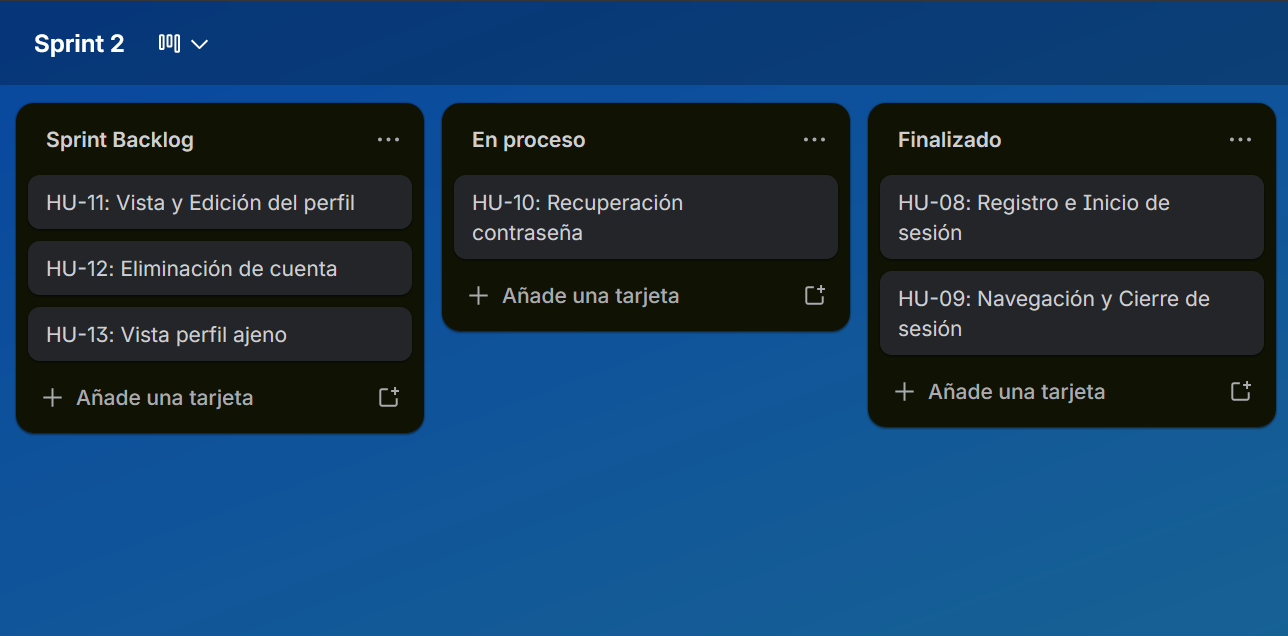
\includegraphics[width=\textwidth]{./imagenes/sprint2-trello.png}
    \caption{Ejemplo de sprint en Trello}
    \label{fig:trello}
\end{figure}



\chapter{Arquitectura del Software}

En el panorama actual del desarrollo de software, la construcción de una aplicación como la que se presenta en este Trabajo de Fin de Grado demanda una plataforma que sea no solo funcional, sino también interactiva, escalable y capaz de gestionar datos de forma dinámica. Para atender esta necesidad, este proyecto se ha desarrollado bajo una arquitectura full-stack, un enfoque integral que permite desacoplar la interfaz de usuario (frontend) de la lógica de negocio (backend) que accede y manipula la base de datos. Esta arquitectura se ilustra de forma esquemática en la siguiente figura.

\begin{figure}[H]
    \centering
    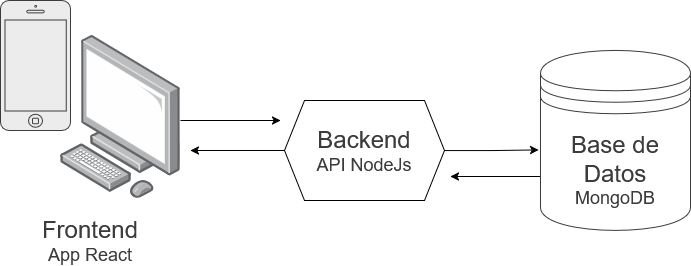
\includegraphics[width=0.9\textwidth]{./imagenes/fullstack.drawio.png}
    \caption{Arquitectura full-stack}
    \label{fig:fullstack}
\end{figure}

Al estructurar el backend exclusivamente como una API, se garantiza que el frontend sea una entidad independiente que consume recursos de forma asíncrona, optimizando la carga y mejorando la experiencia de usuario. Al decir que es una entidad independiente, se estrapola que esta API podría ser utilizada por otras aplicaciones que se construyan a futuro y quieran acceder a los servicios que la API ofrece. Esta es razón de más para testear los métodos de la API mediante la herramienta de pruebas Postman en lugar de solamente desde el frontend, dado que ayudará a comprobar y asegurar el correcto funcionamiento de éstos de forma individual, precisa y documentada.

Además, para llevar a cabo esa tarea de optimización del frontend, se ha relegado el máximo de tareas lógicas y computacionales posibles al backend. Por ejemplo, si la aplicación de React precisa de un conjunto de datos paginados, es la API la que se encargará de la paginación de estos datos, es decir, de servir estos datos por páginas mediante métodos más precisos en lugar de entregar todos los datos de golpe y dejar que el frontend los pagine, puesto que esto lo ralentizaría.

Esta sección analiza el diseño de este ecosistema, detallándolo en estas cuatro secciones:

\begin{itemize}
    \item \textbf{Stack seleccionado}: Justificación del conjunto de tecnologías escogido para el desarrollo de este proyecto de software.
    \item \textbf{Modelado de Datos NoSQL}: El uso de MongoDB y Mongoose para estructurar la información de forma flexible mediante documentos JSON modelados, facilitando el almacenamiento de estructuras de datos.

    \item \textbf{Arquitectura del backend (API REST)}: Se explica la estructura del backend, así como puntos técnicos destacados como la automatización de envío de emails, el mecanismo de autenticación, el almacenamiento de imágenes, y varias técnicas de optimización que se han implementado; y el diseño de los \textit{endpoints} (cada una de las ubicaciones donde la API recibe llamadas) y controladores que implementan las operaciones para gestionar de los datos.

    \item \textbf{Arquitectura del frontend (SPA)}: Recoge el listado de tecnologías específicas empleadas para el frontend de la aplicación, la arquitectura del proyecto, las páginas de la interfaz y, de nuevo, las técnicas de optimización aplicadas.
\end{itemize}

\section{Stack tecnológico seleccionado}

El stack tecnológico es el conjunto de herramientas, programas, aplicaciones u otras piezas de software que son utilizadas para la creación de un producto tecnológico. Una vez estudiadas las principales opciones para el desempeño de cada sector del proyecto, se cuenta con una visión global lo suficientemente rica como para hacer una elección que se ajuste a las necesidades y preferencias del proyecto y su desarrollador.

En esta sección se expone cada punto de esta selección:

\begin{itemize}
    \item Para el desarrollo del frontend de esta aplicación se ha optado por \textbf{Next.js} debido a sus ventajas en rendimiento, optimización para SEO y compatibilidad con React, que es una de las tecnologías más populares e innovadoras hoy en día, por lo que dominarlo resulta de gran interés. Entre los aspectos más atractivos de esta opción se encuentra también que cuenta con una plataforma de lanzamiento y hosting de aplicaciones gratuito, rápido y simple: Vercel; además de que la configuración inicial de un proyecto web se hace muy sencilla y existe una documentación rica, una comunidad activa y numerosos recursos para facilitar el desarrollo web.
    \item En el backend, se ha elegido \textbf{Node.js con Express} por su flexibilidad y el beneficio de utilizar el mismo lenguaje de programación, JavaScript, en todo el stack de desarrollo. Además, se trata de una tecnología ampliamente utilizada en el desarrollo de microservicios y cuenta con librerías que facilitan el acceso al tipo de base de datos que se utilizará.
    \item En cuanto a la base de datos, se ha decidido emplear \textbf{MongoDB} por su modelo flexible y su capacidad para manejar estructuras de datos dinámicas y en formato JSON, el mismo en que se manejan las estructuras de información en JavaScript. También, al ser las bases de datos relacionales las más trabajadas durante el grado, resulta de especial interés cultivar nuevas habilidades con modelos no relacionales como el de MongoDB.
    \item Para el consumo de APIs se usará \textbf{Axios} frente a FetchAPI por simplicidad y aceleración del desarrollo, dado que Axios ofrece más funcionalidades listas para usar como la conversión automática a formato JSON, el manejo de tokens o el manejo de errores integrado; mientras que Fetch, aunque es más ligero, requiere más código manual para tareas frecuentes. Dado que en esta aplicación se implementará autentifación de usuarios y una cantidad considerable de funciones, Axios se presenta como la opción más cómoda y compatible con el resto del stack.
    \item Como herramienta de pruebas de la API, se utiliza \textbf{Postman} frente a Insomnia por una razón principal: la comodidad de tenerlo ya instalado y estar familiarizada, al estar trabajando con ello en otros proyectos personales.
\end{itemize}
\begin{comment}
    \item Las inteligencias artificiles generativas que se han empleado durante la construcción del proyecto son ChatGPT para temas de investigación y clarificación de documentación, y el chat integrado de Github Copilot en Visual Studio Code por la comodidad que ofrece al trabajar directamente sobre el contexto completo del código, haciendo más eficiente y completo tanto el debugging como la entrega de propuestas de optimización y otras mejoras de los componentes y páginas.
    Por el momento, no se ha escogido ninguna plataforma de computación en la nube porque el alcance del proyecto no requiere todavía un despliegue en producción que incluya el uso de servicios externos.
\end{comment}


\subsubsection{Calidad del Código}
Adicionalmente, tanto en el frontend como en el backend, se han empleado varias herramientas destinadas a asegurar la calidad del código:

\begin{itemize}
    \item ESLint: herramienta de análisis estático configurada con reglas para mantener consistencia de código, es decir, un estilo limpio y homogéneo entre los distintos componentes, páginas y otros archivos auxiliares. También ayuda a detectar posibles errores en el código, como variables o importaciones no utilizadas.\cite{eslint_docs}
    \item TypeScript: proporciona verificación de tipos de datos en tiempo de compilación, lo cual permite detectar incompatibilidades en las propiedades de los componentes, llamadas a funciones mal tipadas, o en ocasiones el uso incorrecto de estados.
    \item Prettier: se trata de un formateador automático de código que garazantiza una aparencia consistende de este. Se han configurado reglas para limitar la longitud de línea (\texttt{printWidth: 80}), definir una indentación consistente (\texttt{tabWidth: 2}), forzar el punto y coma al final de las sentencias (\texttt{semi: true}), y estandarizar el uso de comillas dobles (\texttt{singleQuote: false}), entre otras.\cite{prettier_docs}
\end{itemize}
\section{Modelado de datos}

Para la persistencia de la información se ha optado por MongoDB, una base de datos NoSQL orientada a documentos que aporta gran flexibilidad para evolucionar el esquema ágilmente. Aunque no es estrictamente necesario al usar MongoDB, se ha optado por utilizar la librería Mongoose como ODM para definir esquemas, tipos de datos y reglas de validación para facilitar el manejo de los datos y garantizar la integridad de estos.

Así, se han estructurado los datos en diferentes colecciones, cada una de las cuales guarda registros con varios campos de diferentes tipos de datos. El modelado de datos sigue el siguiente esquema.

\begin{figure}[H]
\centering
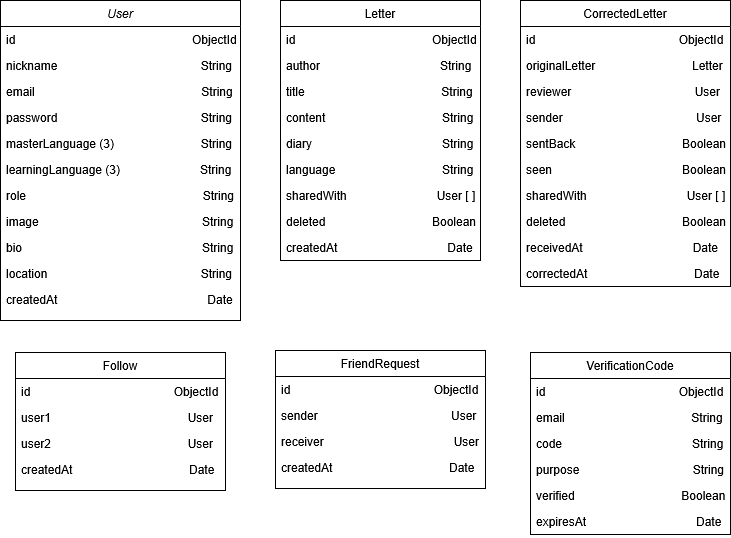
\includegraphics[width=0.8\textwidth]{./imagenes/letterexDB.png}
\caption{Estructura de Datos}
\label{fig:letterexDB}
\end{figure}

En el diseño destaca el uso del ObjectId, un identificador hexadecimal de 12 bytes que garantiza unicidad y permite la indexación eficiente basada en \textit{timestamps}. Además, facilita la vinculación mediante referencias entre colecciones. Cabe mencionar que, aunque internamente se usa \texttt{\_id}, el backend lo transforma en \texttt{id} antes de enviarlo al frontend para ofrecer una interfaz más limpia y desacoplada.

A continuación, se describen las colecciones del sistema:

\begin{itemize}
\item \textbf{Usuario (User):} gestiona la identidad y el perfil del usuario. Incluye su nombre de usuario, email, rol, imagen de perfil, biografía, localidad, contraseña, los idiomas que aprende y conoce (limitados a tres entradas por optimización técnica) y la fecha de creación.
Por seguridad, no se almacena el texto plano de la contraseña, sino que se utiliza la librería \textbf{bcrypt} con un factor de coste (\textit{salting}) de 10 para cifrar la clave antes de su persistencia. El salting es un parámetro que determina la complejidad computacional del hash para dificultar ataques de fuerza bruta al aumentar el tiempo de procesamiento necesario. Se ha escogido 10 por ser el estándar actual en la industria, aquel que se considera el punto de equilibrio óptimo entre seguridad y rendimiento. Cada vez que se quiera comprobar la contraseña, se hashea la entrada con el mismo salting y se compara el resultado con el valor guardado en la base de datos, de forma que ni el administrador ni un atacante pueda tener acceso a la contraseña.

\item \textbf{Carta (Letter):} almacena los textos originales. Contiene el author (referencia al usuario creador), título, contenido, diario, idioma y fecha de creación. También incluye un array de referencias a los usuarios con que se comparte la carta (\textit{sharedWith}) y un campo \textit{deleted} para el borrado lógico, permitiendo que los receptores conserven sus correcciones.

\item \textbf{Carta Corregida (CorrectedLetter):} gestiona el flujo de revisión. Vincula la corrección a la carta original mediante le referencia \textit{originalLetter}, además de referenciar al revisor o receptor de la carta (\textit{reviewer}) y a su autor (\textit{sender}). Controla los estados de envío de vuelta mediante el booleano \textit{sentBack}, y de si el receptor vio ya la nueva carta que le llegó con el booleano \textit{seen}, de forma que en el frontend se puedan crear etiquetas de "Nuevo" a modo de notificación. También, guarda la fecha de envío y de corrección (envío de vuelta) de la carta.

\item \textbf{Amistad (Follow):} gestiona el grafo social mediante referencias a \textit{user1} (seguidor) y \textit{user2} (seguido), facilitando el intercambio de correcciones y el listado de amigos y usuarios sugeridos.

\item \textbf{Solicitud de Amistad (FriendRequest):} capa intermedia para peticiones de amistad entre un usuario \textit{sender} y un usuario \textit{receiver}. Es una colección efímera: al aceptar o rechazar, el documento se elimina, creando el vínculo en la colección \textit{Follow} en caso de aceptación.

\item \textbf{Código de Verificación (VerificationCode):} entidad de apoyo para la validación de registros y recuperación de claves. Almacena el código hasheado, el email del usuario implicado, un campo \textit{verified} que indica si ya ha sido utilizado, y un campo \textit{purpose} que indica si sirve para un registro o para una recuperación de contraseña. Además, se utiliza un índice TTL (Time To Live) en el campo \textit{expiresAt}, que sirve para que MongoDB elimine automáticamente los códigos al cabo de 7 minutos de su creación.

\end{itemize}
\section{Arquitectura del backend}

En esta sección se expone cómo está estructurado el servidor del proyecto, los flujos lógicos que sigue, varios puntos interesantes sobre su funcionamiento, y las diferentes rutas con las que cuenta la API.

\subsection{Estructura del backend}
El servidor se organiza en módulos interconectados para ofrecer servicios robustos al frontend y facilitar un desarrollo escalable.
Una petición HTTP sigue esta secuencia: el cliente consume una ruta (endpoint), se ejecutan los middlewares de autenticación y/o carga de imágenes si corresponde, y un controlador procesa los datos interactuando con uno o varios modelos para luego devolver la respuesta que corresponda. Por ello, se distinguen los siguientes modulos principales:

\begin{itemize}
    \item \textbf{Entrada y Configuración Inicial}: En la raíz del proyecto se encuentra el archivo \texttt{index.js}, encargado de configurar y levantar el servidor. Para ello, se conecta a la base de datos y carga los endpoints y los middlewares pertinentes.

    Para que el frontend tenga acceso a la API, es esencial configurar el mecanismo de seguridad \textbf{CORS (Cross-Origin Resource Sharing)}. En una arquitectura desacoplada como la de este proyecto, el cliente y el servidor suelen operar en dominios o puertos distintos. Por seguridad, los navegadores modernos aplican la "Política de Mismo Origen" (\textit{Same-Origin Policy}), que prohíbe que un script cargado en un origen acceda a recursos de otro distinto. Con la configuración de \texttt{CORS} se define una lista de dominios autorizados a acceder a la API, así como habilitar el intercambio de credenciales.

    \begin{figure}[h]
    \centering
    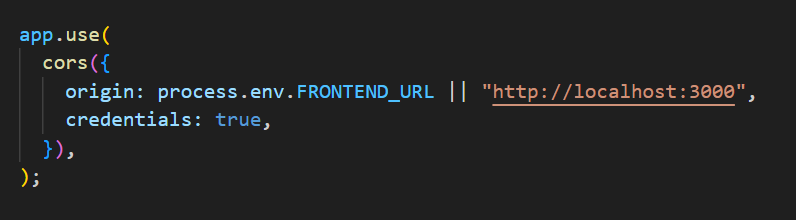
\includegraphics[width=0.8\textwidth]{imagenes/cors.png}
    \caption{Configuración del CORS en la entrada del backend}
    \label{fig:cors}
    \end{figure}

    \item \textbf{Lógica de negocio}: la lógica de negocio se organiza en una estructura con tres partes, basándose en el principio de separación por responsabilidades ("SoC" o Separation of Concerns), que busca dividir sistemas complejos en partes más pequeñas y manejables cada una de las cuales cubre una funcionalidad. Así, tenemos la definición de los puntos de acceso (\texttt{routes/}), la implementación de las reglas de negocio (\texttt{controllers/}) y la definición de los modelos de datos (\texttt{models/}).

    \item \textbf{Middlewares}: La carpeta (\texttt{middlewares/}) incluye las configuraciones de autenticación de usuario y de subida de archivos, que se explicarán en detalle más adelante.
\end{itemize}

Además, el proyecto cuenta con la carpeta \texttt{templates/}, que contiene la plantilla para enviar correos automatizados; y la carpeta \texttt{uploads/profile\_pictures/}, que actúa como almacenamiento local para las imágenes de perfil de los usuarios.


Esta separación garantiza que el sistema sea escalable y fácil de mantener.


\subsection{Emails automatizados}
La función del backend encargada la generación de códigos de verificación y su envío via email al usuario, que se emplea tanto para el registro de una nueva cuenta como para la recuperación de sus credenciales en caso de olvido; es capaz de realizar sus tareas de forma automatizada gracias a un transportador que utiliza el servicio SMTP (Simple Mail Transfer Protocol, un protocolo de red para intercambiar mensajes de correo electrónico) de Gmail. Un transportador es un objeto de configuración donde se define este servicio SMTP y se inyectan las credenciales para utilizarlo, es decir, la cuenta de correo electrónico y su contraseña.

En realidad, ya no se utiliza la contraseña de la cuenta de correo directamente, Google bloqueó eso por ser una práctica poco segura y la sustituyó por Google App Password, códigos de 16 caracteres que se pueden obtener en la configuración de la cuenta de Google y que actúan como las credenciales para usar nuestra cuenta de correo de Gmail mediante código. Estas credenciales se pueden obtener solamente al tener la 2FA (2 Factor Authentication) de Google activada, y se pueden revocar de una aplicación u otra cuando se necesite; manteniendo así las credenciales primarias seguras.

Lo que se envía en estos correos automatizados es una plantilla HTML con el código de verificación generado. De esta forma, el email que reciben los usuarios es visualmente agradable y fácil de entender en un vistazo. Así es como se ve:

\begin{figure}[H]
    \centering
    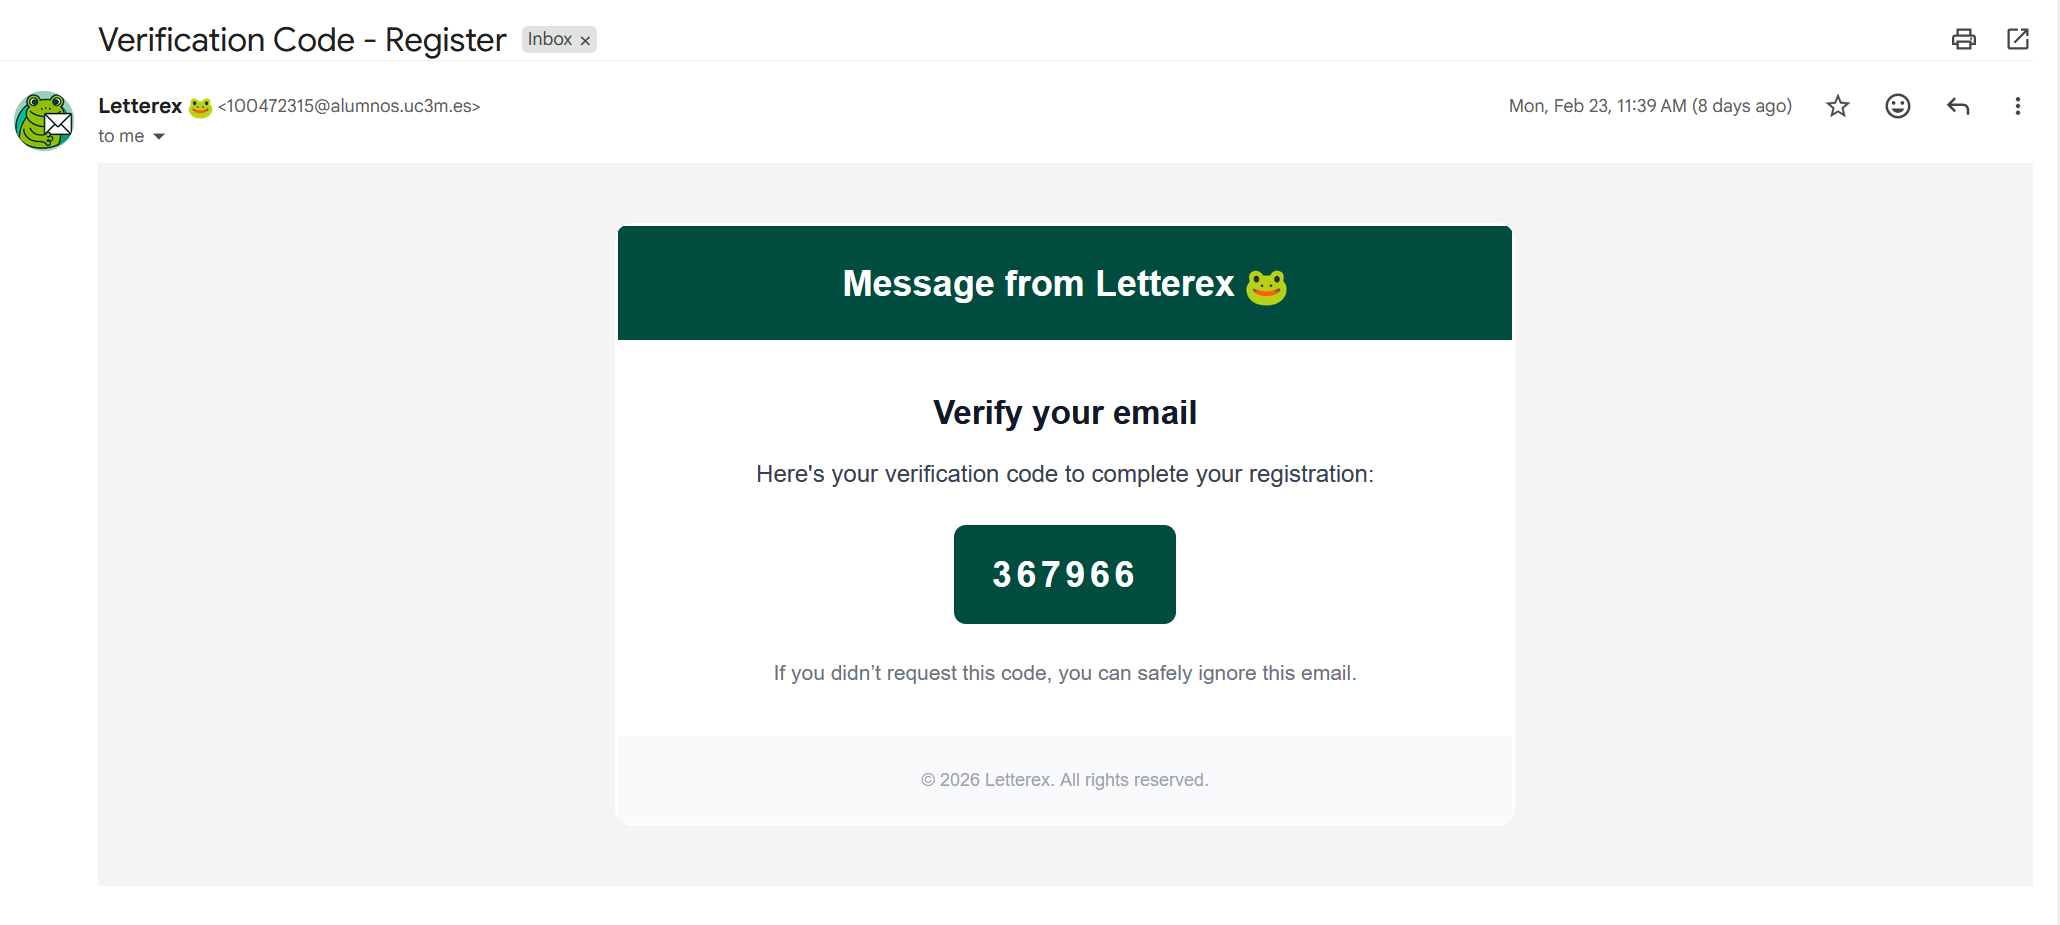
\includegraphics[width=\textwidth]{./imagenes/template_email.png}
    \caption{Email automatizado}
    \label{fig:email}
\end{figure}

\subsection{Mecanismo de Autenticación y Autorización}
Al acceder a la plataforma introduciendo su nombre de usuario o email y contraseña, el usuario recibe un token que contiene información de la sesión como el momento en que inició, el momento de caducidad, y los datos no sensibles del usuario. Se trata de un token JWT (JSON Web Token) \cite{jwtio}, un contenedor de información seguro y compacto que permite verificar la identidad del cliente en cada interacción con la API.

\begin{figure}[H]
    \centering
    
\includegraphics[height=3cm]{./imagenes/jwt.png}
    \caption{JSON Web Tokens}
    \label{fig:jwt}
\end{figure}

Este token se envia desde el backend y se almacena en el navegador mediante \textit{cookies}, con el objetivo de que el navegador pueda recordar la sesión del usuario. Al cerrar la sesión, esta cookie se elimina. El navegador adjunta automáticamente el token a las solicitudes HTTP que envía al servidor. De esta forma, el servidor es capaz de identificar al usuario y aplicar los permisos correspondientes sin necesidad de consultar una tabla de sesiones activa en la base de datos, lo que optimiza los recursos del sistema.

Sobre el refuerzo de la seguridad de la cookie, hay dos puntos interesantes que mencionar. En primer lugar, la cookie es HttpOnly, es decir, no se puede leer mediante JavaScript sino que solo puede leerla el navegador. De esta forma, el token está protegido contra ataques maliciosos como \textbf{Cross-Site Scripting (XSS)}, una vulnerabilidad en la que un atacante inyecta y ejecuta código malicioso (generalmente de JavaScript) en el navegador de otros usuarios que usan la aplicación.

En segundo lugar, se ha implementado el atributo \textbf{SameSite} con el valor \texttt{"Strict"}. Esta configuración es una medida de seguridad crítica para prevenir ataques de tipo \textbf{CSRF (Cross-Site Request Forgery)}, que aprovechan la naturaleza automática de los navegadores, dado que estos adjuntan las cookies de sesión a cualquier petición dirigida al dominio de origen. El atacante podría engañar a un usuario autenticado para que haga clic en un enlace malicioso en una pestaña diferente, y dicho enlace dispararía una petición a nuestra API (por ejemplo, para borrar una carta o cambiar la contraseña). Con la configuración de SameSite, este tipo de ataques son mitigados.

Al llegar una solicitud HTTP al sistema, si se trata de una ruta protegida se ejecuta el \textbf{Middleware de Autenticación}. Este componente intercepta la solicitud, extrae el token JWT de la cookie y verifica su validez. Si es válido, el middleware decodifica la información del usuario y la inyecta en el objeto de la petición, permitiendo que el resto del flujo identifique al autor de la acción, es decir, el usuario autenticado en la aplicación.

Estas decisiones técnicas refuerzan la robustez del sistema y aseguran que cada acción realizada en este sea legítima y provenga exclusivamente de la interacción directa del usuario con la interfaz oficial, de forma que usuario pueda acceder de forma segura a las acciones que requieren su autenticación.

\subsection{Almacenamiento de imágenes con Multer y Cloudinary}

Para la gestión de imágenes de perfil, se ha implementado una solución que combina la librería \textbf{Multer} para el procesamiento eficiente de archivos con \textbf{Cloudinary} como servicio de almacenamiento en la nube. Multer es una librería que facilita la subida de archivos mediante formularios web para aplicaciones de Node.js. Por su parte, Cloudinary es un servicio de gestión de recursos digitales, en especial imágenes y vídeos, que proporciona almacenamiento persistente en la nube y optimización automática. \cite{llamas_multer_nd, cloudinary_official_2026,moge_cloudinary_2026}

La configuración del sistema de subida de archivos se divide en tres pilares fundamentales:

\begin{itemize}
    \item Procesamiento en memoria: Se utiliza Multer para interceptar y procesar la subida de archivos directamente en memoria con un búfer, evitando la necesidad de almacenamiento temporal en disco. Una decisión de diseño clave ha sido el renombrado del archivo por el identificador del usuario extraído del token de autenticación, de modo que cada usuario posea una única imagen de perfil en Cloudinary. En caso de actualización, se sobrescribe la imagen anterior automáticamente, eliminando la necesidad de gestionar manualmente archivos obsoletos.

    \item Almacenamiento en la nube: Una vez procesado el búfer, la imagen se sube directamente a Cloudinary. El sistema almacena la URL segura retornada por Cloudinary en la base de datos, facilitando un acceso rápido sin depender del almacenamiento local del servidor. Además, Cloudinary aplica transformaciones automáticas, como la limitación de dimensiones a 800x800 píxeles, para garantizar consistencia visual y reducir consumo de ancho de banda.
    \item Filtrado de seguridad: Para prevenir la subida de archivos maliciosos (como \textit{scripts} ejecutables disfrazados), se ha implementado un filtro por tipo MIME y extensión. El sistema solo acepta formatos de imagen estándar (\texttt{JPEG, JPG, PNG}), verificando tanto la extensión del archivo como su tipo MIME real para asegurar la integridad del recurso. También, se establece un máximo de tamaño del archivo de 5 MB para evitar \textbf{ataques de denegación de servicio (DoS)} por agotamiento de almacenamiento o ancho de banda.

\end{itemize}

Este módulo se exporta como un middleware independiente, lo que permite inyectarlo exclusivamente en las rutas de la API que requieren capacidad de subida, manteniendo así el principio de responsabilidad única en el código. Además, la integración con Cloudinary elimina la dependencia de la infraestructura local de almacenamiento, proporcionando escalabilidad y disponibilidad.

\subsection{Interfaz de Programación de Aplicaciones (API): Rutas y Controladores}

El backend de la plataforma actúa como una capa de servicios diseñada para que el frontend interactúe con la base de datos de forma segura y eficiente. Esta comunicación se articula mediante una \textbf{API RESTful}, que expone una serie de puntos de entrada o endpoints organizados por recursos (usuarios, cartas, correcciones, etc.).

La lógica de interacción se fundamenta en las operaciones \textbf{CRUD} (\textit{Create, Read, Update, Delete}), que representan las acciones esenciales para la gestión de persistencia de datos. En este proyecto, dichas acciones se mapean directamente con los métodos del protocolo \textbf{HTTP}, garantizando una arquitectura estandarizada:

\begin{itemize}
    \item \textbf{POST (Create)}: Utilizado para la creación de nuevos documentos, como el registro de un usuario o el envío de una nueva carta.
    \item \textbf{GET (Read)}: Empleado para la recuperación de información, ya sea una lista de recursos o un documento específico identificado por su ID.
    \item \textbf{PUT / PATCH (Update)}: Destinados a la actualización de registros existentes. Se utiliza \texttt{PUT} para sustituciones integrales y \texttt{PATCH} para modificaciones parciales, como marcar una carta como "leída".
    \item \textbf{DELETE (Delete)}: Encargado de la eliminación de recursos o, en el caso de las cartas, de la activación del borrado lógico mencionado anteriormente.
\end{itemize}

Cada ruta definida en el servidor está vinculada a un \textbf{controlador} específico, el cual contiene la lógica final para procesar la solicitud. Una vez superada la fase de autenticación, la ejecución pasa al controlador específico correspondiente, cuya función es extraer los parámetros de la consulta, utilizar la identidad del usuario ya validada para aplicar reglas de negocio, ejecutar las operaciones correspondientes en MongoDB mediante los modelos de Mongoose, y devolver una respuesta HTTP con los datos en formato JSON y un código de éxito o error.

A continuación, se muestra una tabla con todos los métodos que se han desarrollado para esta API y de los que el frontend más adelante se servirá. Estás separados en categorías según el controlador y enrutador que se encarga de ellos: User, Letter, CorrectedLetter y Follow. Podría crearse uno nuevo para los modelos de VerificationCode y FriendRequest, pero por simplicidad se han incluido las pocas funciones de estos en el grupo de User y Follow, respectivamente. Además, se marca con un asterisco los valores de entrada obligatorios.

\begin{longtable}{|l|p{5cm}|p{8cm}|}
\hline
\textbf{Función} & \textbf{Ruta} & \textbf{Descripción} \\
\hline
\endhead
\hline
\endfoot
\multicolumn{3}{|c|}{\textbf{User Routes}} \\
\hline
POST & /api/users/register & Registrar un nuevo usuario. \newline \textbf{Valores de entrada:} nickname*, email*, password*, master\-Language*, learning\-Language* \newline \textbf{Valores de salida:} status, message, user \\
POST & /api/users/login & Iniciar sesión. Si las credenciales recibidas son correctas, se crea y envía la cookie de autenticación. \newline \textbf{Valores de entrada:} email* (string, puede ser email o nickname), password* \newline \textbf{Valores de salida:} status, userData, token, cookie authToken \\
POST & /api/users/logout & Cerrar la sesión. Se limpia la cookie de autenticación. \newline \textbf{Valores de entrada:} ninguno \newline \textbf{Valores de salida:} status, message \\
GET & /api/users/profile/:id? & Obtener los datos del perfil de usuario cuyo id es especificado en la ruta, o en su defecto (es un parámetro opcional, de ahí el signo de interrogación en la ruta) del usuario autenticado.\newline \textbf{Valores de salida:} status, user \\
GET & /api/users/list-users/:page? & Listar usuarios con paginación. Si no se recibe el parámetro page, que indica la página que se pide, se entregan los usuarios de la primera página. \newline \textbf{Valores de salida:} status, users, page, itemsPerPage, totalUsers, totalPages \\
PUT & /api/users/update & Actualizar datos del usuario autenticado. \newline \textbf{Valores de salida:} status, userData \\
PUT & /api/users/change-password & Cambiar contraseña actual. \newline \textbf{Valores de salida:} status, message \\
PUT & /api/users/profile-picture & Subir foto de perfil. Se trata de un método PUT porque no solo sube una nueva imagen al sistema de archivos sino que modifica los datos del usuario.\newline \textbf{Valores de salida:} status, userId, profilePicture \\
DELETE & /api/users/profile-picture & Eliminar foto de perfil. \newline \textbf{Valores de salida:} status, message \\
GET & /api/users/profile-picture/:id & Obtener foto de perfil de un usuario. En caso de que el parámetetro id no esté especificado, se entrega la del usuario autenticado. \newline \textbf{Valores de salida:} Archivo (imagen) \\
GET & /api/users/check-nickname/:nickname & Verificar disponibilidad de nickname. \newline \textbf{Valores de salida:} status, inUse: boolean \\
GET & /api/users/check-email/:email & Verificar si email está registrado. \newline \textbf{Valores de salida:} result, inUse: boolean \\
POST & /api/users/verification-code & Enviar código de verificación. \newline \textbf{Valores de entrada:} email*, purpose \newline \textbf{Valores de salida:} message \\
POST & /api/users/check-code & Verificar código de verificación. \newline \textbf{Valores de entrada:} email*, code*, purpose \newline \textbf{Valores de salida:} status, message \\
PUT & /api/users/reset-password & Restablecer contraseña con código de verificación. \newline \textbf{Valores de salida:} status, message \\
DELETE & /api/users/delete-account & Eliminar cuenta de usuario. \newline \textbf{Valores de salida:} status, message \\
\hline
\hline
\multicolumn{3}{|c|}{\textbf{Letter Routes}} \\
\hline
POST & /api/letters/new & Guardar una carta nueva. \newline \textbf{Valores de entrada:} title*, content*, language*, created\_at*, diary \newline \textbf{Valores de salida:} status, message, letter \\
GET & /api/letters/view/:letterId & Obtener información y contenido de una carta.\newline \textbf{Valores de salida:} status, letter, sharedWithDetails \\
PUT & /api/letters/edit/:id & Editar una carta existente. \newline \textbf{Valores de salida:} status, message, letter \\
PUT & /api/letters/edit-diary & Editar el diario de una carta. \newline \textbf{Valores de salida:} status, message, letter \\
DELETE & /api/letters/delete/ & Eliminar una o varias cartas. \newline \textbf{Valores de salida:} status, message \\
GET & /api/letters/list & Listar todas las cartas del usuario. \newline \textbf{Valores de salida:} status, letters, count \\
GET & /api/letters/list/search & Buscar cartas por título. \newline \textbf{Valores de salida:} status, letters \\
POST & /api/letters/share/:id & Compartir una carta con otro usuario (uno o varios). \newline \textbf{Valores de entrada:} shared\-With* \newline \textbf{Valores de salida:} \{message, letter, correctedLetters\} \\
GET & /api/letters/diaries & Listar diarios del usuario. \newline \textbf{Valores de salida:} status, diaries \\
GET & /api/letters/count/:id? & Contar cartas por idioma. Si no se especifica id en la ruta, se cuentan las del usuario autenticado. \newline \textbf{Valores de salida:} Array de \{language, count\} \\
\hline
\hline
\multicolumn{3}{|c|}{\textbf{Follow Routes}} \\
\hline
POST & /api/follow/add/:id & Mandar una solicitud de amistad a un usuario. \newline \textbf{Valores de salida:} status, message \\
DELETE & /api/follow/unfollow/:id & Dejar de seguir a un usuario. \newline \textbf{Valores de salida:} status, message \\
GET & /api/follow/request/:id & Verificar si existe solicitud de amistad. \newline \textbf{Valores de salida:} status, exists: boolean \\
GET & /api/follow/friends & Obtener lista de amigos. \newline \textbf{Valores de salida:} status, count, friends \\
GET & /api/follow/non-friends & Obtener usuarios no agregados. \newline \textbf{Valores de salida:} status, users, totalUsers, totalPages \\
GET & /api/follow/non-friends/:filter & Obtener no usuarios no agregados con un filtro por su nickname. \newline \textbf{Valores de salida:} status, users, totalUsers, totalPages \\
GET & /api/follow/suggested & Obtener usuarios sugeridos. Son usuarios a los que el usuario autenticado no sigue y que tienen idiomas en común con este. \newline \textbf{Valores de salida:} status, suggestedUsers \\
POST & /api/follow/request/:id & Enviar solicitud de amistad. \newline \textbf{Valores de salida:} status, message, friendRequest \\
GET & /api/follow/requests & Listar solicitudes de amistad recibidas. \newline \textbf{Valores de salida:} status, requests \\
POST & /api/follow/accept/:id & Aceptar solicitud de amistad. \newline \textbf{Valores de salida:} status, message \\
POST & /api/follow/decline/:id & Rechazar solicitud de amistad. \newline \textbf{Valores de salida:} status, message \\
\hline
\hline
\multicolumn{3}{|c|}{\textbf{Corrected Letter Routes}} \\
\hline
PATCH & /api/corrected-letters/send-back/:corrected\-Letter\-Id & Mandar de vuelta su autor la carta corregida. \newline \textbf{Valores de salida:} status, message, correctedLetter \\
GET & /api/corrected-letters/corrections/:original\-Letter\-Id & Obtener correcciones de una carta. \newline \textbf{Valores de salida:} status, corrections \\
GET & /api/corrected-letters/corrected\-Letter/:corrected\-Letter\-Id & Obtener corrección específica por ID. \newline \textbf{Valores de salida:} status, correctedLetter \\
GET & /api/corrected-letters/received/ & Obtener cartas recibidas para corregir. \newline \textbf{Valores de salida:} status, correctedLetters, count \\
GET & /api/corrected-letters/received/search & Buscar cartas recibidas por un filtro "search". \newline \textbf{Valores de salida:} status, correctedLetters \\
PUT & /api/corrected-letters/update/:corrected\-Letter\-Id & Actualizar correcciones en proceso. Si la carta ya ha sido enviada de vuelta no se puede realizar esta acción. \newline \textbf{Valores de salida:} status, message, correctedLetter \\
GET & /api/corrected-letters/count/:id? & Contar cartas corregidas por idioma. Si no se especifica el id de usuario en la ruta, se cuentan las del usuario autenticado. \newline \textbf{Valores de salida:} Array de \{language, count\} \\
DELETE & /api/corrected-letters/:corrected\-Letter\-Id & Eliminar carta corregida. \newline \textbf{Valores de salida:} status, message \\
\hline
\caption{Rutas de la API de Letterex}
\label{tab:rutas-api}
\end{longtable}



\subsection{Técnicas de optimización}

\subsubsection{Optimización de búsqueda datos}
La lógica de filtrado se procesa íntegramente en el servidor para garantizar la escalabilidad y mejorar la velocidad de la interfaz liberándola de tareas programacionales. El controlador recibe los términos de búsqueda y ejecuta una consulta optimizada en MongoDB. Esto reduce drásticamente el tamaño de los datos transferidos a través de la red en comparación con un filtrado realizado en el lado del cliente sobre la totalidad de los registros.

Además, para mejorar la usabilidad en la búsqueda y filtrado de cartas, se ha implementado un sistema de comunicación eficiente entre el cliente y el servidor. Donde tenemos una barra de búsqueda, en lugar de realizar peticiones por cada pulsación de tecla, lo que derivaría en un consumo excesivo de recursos y latencia en la red, se ha aplicado la técnica de \textbf{debouncing}. Esta técnica sigue la siguiente lógica:

\begin{itemize}
    \item Control de Eventos: Cuando el usuario escribe en el campo de búsqueda, se inicia un temporizador interno.
    \item Retraso Controlado: Si el usuario sigue escribiendo antes de que transcurran un intervalo definido de tiempo (500ms), el temporizador se reinicia.
    \item Petición Asíncrona: Solo cuando el usuario deja de escribir durante el tiempo estipulado, se dispara la solicitud formal a la API.
\end{itemize}

Así, se logra un consumo y envío de recursos mucho más eficiente.

\subsubsection{Procesamiento Avanzado de Datos: Aggregate de MongoDB}

Otra forma de optimización clave utilizada en el desarrollo del backend es el uso del Aggregate o operaciones de agregación de MongoDB \cite{mongodb_aggregation_2026}. Esta herramienta permite acceder a diferentes colecciones y aplicar filtrados, ordenamientos, uniones, proyecciones y paginación en una única operación atómica. Esto evita el procesar grandes volúmenes de datos en la capa de JavaScript o caer en el problema de las \textbf{N+1 consultas} (realizar múltiples peticiones a la base de datos para completar un solo registro). Así, delegamos la carga de procesamiento al motor de la base de datos, manteniendo tiempos de respuesta bajos y escalables.

\begin{comment}
Un ejemplo real implementado es el flujo de trabajo para la búsqueda de cartas, donde se obtienen también los detalles de los usuarios que han enviado correcciones. El proceso se divide en las siguientes etapas:

    \item \textbf{Pre-filtrado y Paginación}: Primero se selecciona un conjunto reducido de documentos mediante un \texttt{\$match} (autor logueado y carta no eliminada), un \texttt{\$sort} cronológico y las etapas \texttt{\$skip} y \texttt{\$limit} para gestionar la paginación. Realizar esto al inicio asegura que las operaciones posteriores, más costosas, solo se apliquen a los resultados visibles.

    \item \textbf{Resolución de Identidades}: Se aplica un \texttt{\$lookup} (equivalente al \textit{join} de SQL) para unir la colección de cartas con la de usuarios. Esto permite resolver los IDs del array \texttt{sharedWith} y obtener los perfiles reales de los destinatarios.

    \item \textbf{Búsqueda de Correcciones}: Seguidamente, se realiza un segundo cruce con la colección CorrectedLetter. Para cada carta, el sistema busca documentos donde la carta original coincida con la actual y el campo \texttt{sentBack} sea verdadero, agrupando estos resultados en un array interno.

    \item \textbf{Transformación de la Salida}: Finalmente, se formatea la respuesta final procesando el array de amigos mediante el operador \texttt{\$map} de MongoDB. Este transforma cada elemento verificando si el ID del amigo existe en el array de revisores (usando \texttt{\$in}) y extrayendo el ID específico de la corrección mediante la combinación de \texttt{\$filter} y \texttt{\$arrayElemAt}.
\end{comment}

Un ejemplo representativo es el flujo de obtención de cartas junto con la información de sus correcciones y usuarios asociados. La tubería de agregación de MongoDB permite resolver estas múltiples relaciones en una única consulta. El proceso se estructura en las siguientes etapas:

\begin{enumerate}
    \item \textbf{Filtrado y paginación}: Se seleccionan únicamente las cartas del usuario autenticado que no han sido eliminadas, aplicando además ordenación cronológica y paginación. Realizar esto al inicio asegura que las operaciones posteriores, más costosas, solo se apliquen a los resultados deseados.

    \item \textbf{Enriquecimiento de datos}: Se incorporan los datos de los usuarios relacionados, aquellos con los que se ha compartido la carta, mediante operaciones equivalentes a uniones (\textit{joins}), resolviendo los identificadores almacenados en el campo \texttt{sharedWith}.

    \item \textbf{Obtención de correcciones}: Se recuperan las correcciones asociadas a cada carta, filtrando para obtener solamente aquellas que han sido enviadas de vuelta al autor.

    \item \textbf{Transformación de la respuesta}: Finalmente, se construye la estructura de salida combinando la información obtenida, de forma que cada carta incluye los datos necesarios para su representación en la interfaz.
\end{enumerate}

Aunque construir esta lógica requiere mayor tiempo de desarrollo, el uso de la Agregación de MongoDB permite una mejora drástica en el rendimiento del sistema reduciendo el tráfico de red entre el servidor y la base de datos.

A continuación se muestra el código de la función que se ha presentado como ejemplo de su uso.

\begin{figure}[H]
    \centering
    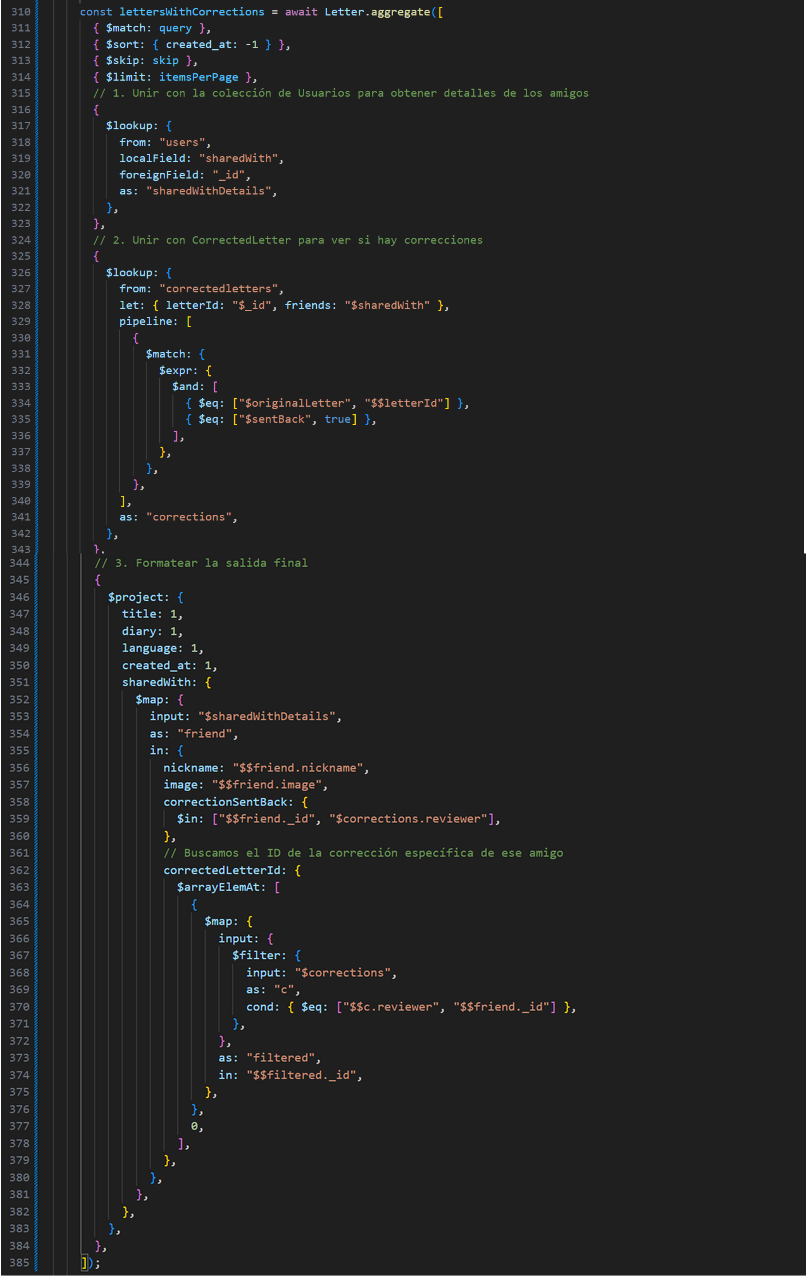
\includegraphics[width=\textwidth]{./imagenes/aggregate3.png}
    \caption{Consulta optimizada 1}
    \label{fig:aggregate}
\end{figure}
\section{Frontend de la aplicación}

El frontend ha sido desarrollado como una aplicación web moderna y responsiva, utilizando las últimas tecnologías del ecosistema React. En esta sección, se presentan las diferentes tecnologías que han intervenido en el desarrollo de esta pieza de software, la arquitectura que sigue el proyecto de frontend, las diferentes páginas que lo componen, y varias técnicas de optimización que se han empleado.


\subsection{Stack Tecnológico}

La aplicación se ha construido utilizando el siguiente stack tecnológico:

\begin{itemize}
    \item React 19: Biblioteca principal para la construcción de interfaces de usuario basadas en componentes.
    \item Next.js 15: Framework de React que proporciona renderizado del lado del servidor (SSR), enrutamiento basado en archivos y optimizaciones de rendimiento automáticas.
    \item TypeScript: Superset tipado de JavaScript que proporciona seguridad de tipos en tiempo de compilación.
    \item Tailwind CSS: Framework de CSS utility-first para un desarrollo de estilos rápido y consistente. El uso este librería agiliza la aplicación de interfaces responsivas, adaptándose a todo tipo de dispositivos con tamaños de pantalla diversos.
    \item Framer Motion: Biblioteca de animaciones para crear transiciones fluidas y experiencias interactivas.\cite{framer_motion_docs}
    \item React Quill: Editor de texto enriquecido basado en Quill.js para la escritura de cartas.\cite{quill_react_playground}
    \item Axios: Cliente HTTP para comunicación con la API backend.
    \item React Leaflet: Biblioteca para integración de mapas interactivos.\cite{react_leaflet_docs}
\end{itemize}

\subsection{Arquitectura del Frontend y Gestión del Estado}

El proyecto sigue la estructura de \textit{App Router} de Next.js 13+, que organiza las rutas de la aplicación en función de la estructura de directorios. La estructura consta de las siguientes capas:

\begin{itemize}
    \item \texttt{app/}: Directorio principal que contiene las páginas y rutas de la aplicación. Cada subcarpeta se convierte en una ruta de la web automáticamente si incluimos dentro un archivo \texttt{page.tsx}.
    \item \texttt{components/}: Componentes reutilizables de la interfaz de usuario.
    \item \texttt{services/}: Capa de servicios que encapsula las llamadas a la API.
    \item \texttt{context/}: Contextos de React para gestión de estado global.
    \item \texttt{lib/}: Utilidades, tipos de TypeScript y constantes.
    \item \texttt{stylesheets/}: Aunque los estilos se aplican mayoritariamente con Tailwind CSS, para ciertos casos se utilizan estilos personalizados complementarios compartidos por varios componentes.
\end{itemize}


Para facilitar la escalabilidad y la reutilización del código, se han desarrollado \textbf{componentes reutilizables} para encapsular elementos como botones, inputs, selectores, descripciones emergentes, etc. Estos se incluyen en diferentes páginas y componentes de la aplicación para garantizar patrones de diseño consistentes, evitar la duplicación de lógica, y facilitar la implementación de cambios globales.

En cuanto a la \textbf{comunicación con el backend}, la capa de servicios encapsula toda la lógica de acceso a la API, que se implementa con Axios. La capa incluye cuatro módulos diferenciados por funcionalidad: usuarios, cartas, correcciones y amistades. Cada módulo de servicio exporta funciones asíncronas que manejan configuración de headers de autenticación, errores HTTP y de Axios, transformación de datos entre el formato de la API y el formato esperado por los componentes; y validación básica de datos antes del envío.

Respesto a la gestión del estado de la aplicación, se deben almacenar ciertos datos comunes a todas o varias páginas, así como datos individuales de cada página o componente. Para ello, se utilizan múltiples estrategias:

\begin{itemize}
    \item \textbf{Local Storage}: Utilizado para datos no sensibles de la experiencia de usuario, como la preferencia de tema (modo claro u oscuro), que se establece inicialmente como el que tenga por defecto el usuario en su navegador, pero puede ser configurarse desde el menú desplegable de Letterex.
    \item \textbf{React Hooks}: Se usan funciones especiales de React como \texttt{useState}, \texttt{useEffect} o \texttt{useRef}, para controlar el estado local de los componentes. Este último se usa para implementar una caché en memoria por página, por ejemplo, guardando resultados paginados. Cuando el usuario vuelve a una página ya consultada, los datos se leen desde caché y se muestran al instante. Así, se consigue una mejora del rendimiento por la reducción de llamadas redundantes al servidor.
    \item \textbf{Context API}: guarda el estado del componente para gestionar diálogos modales de forma centralizada, evitando \textit{prop drilling}, fenónemo en que los componentes se pasan datos de padres a hijos sucesivamente quedando varios hijos intermedios que no los utilizan. Con un proveedor de contexto, la app es capaz de renderizar un solo componente de diálogo que se abre y se cierra con dos funciones a las que cualquier componente puede acceder fácilmente, en este caso mediante un hook personalizado llamado \texttt{useDialog} que devuelve el contexto del diálogo. Por ejemplo, la siguiente figura muestra la función que abrirá el diálogo de error a su derecha. Esta estrategia se utiliza también para guardar los datos no sensibles del usuario autenticado.

    \begin{figure}[H]
        \centering
        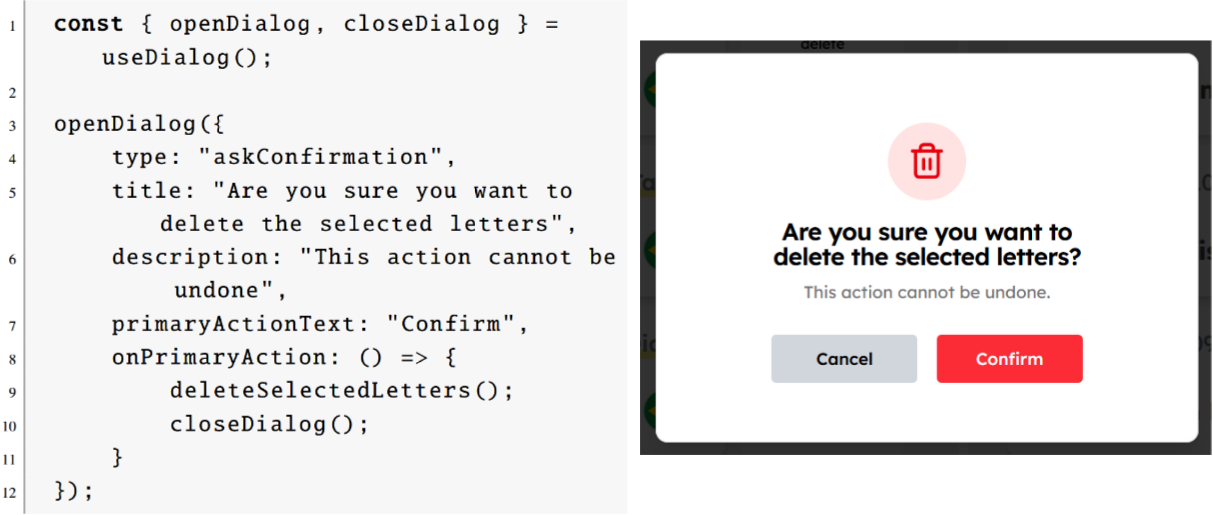
\includegraphics[width=\textwidth]{imagenes/ui/dialogDeleteAll.png}
        \caption{Código de apertura del diálogo y resultado en la interfaz}
        \label{fig:dialog}
    \end{figure}

\end{itemize}



\subsection{Páginas de la aplicación}

En este apartado se irán mostrando las diferentes páginas que componen la interfaz, que en total son siete: la página de inicio de sesión, la página principal, la página para la creación de una nueva carta, la página de correción de cartas recibidas, la página de visualización de una correción recibida, la página de amigos, y la página de perfil de usuario.

En las paginas protegidas (aquellas a las que se accede tras iniciar sesión), el componente \texttt{Sidebar} envuelve todo el contenido para proporcionar una barra lateral de navegación persistente con acceso rápido a todas las páginas de la aplicación.

\subsubsection{Página de Inicio y Autenticación}

\begin{figure}[h]
    \centering
    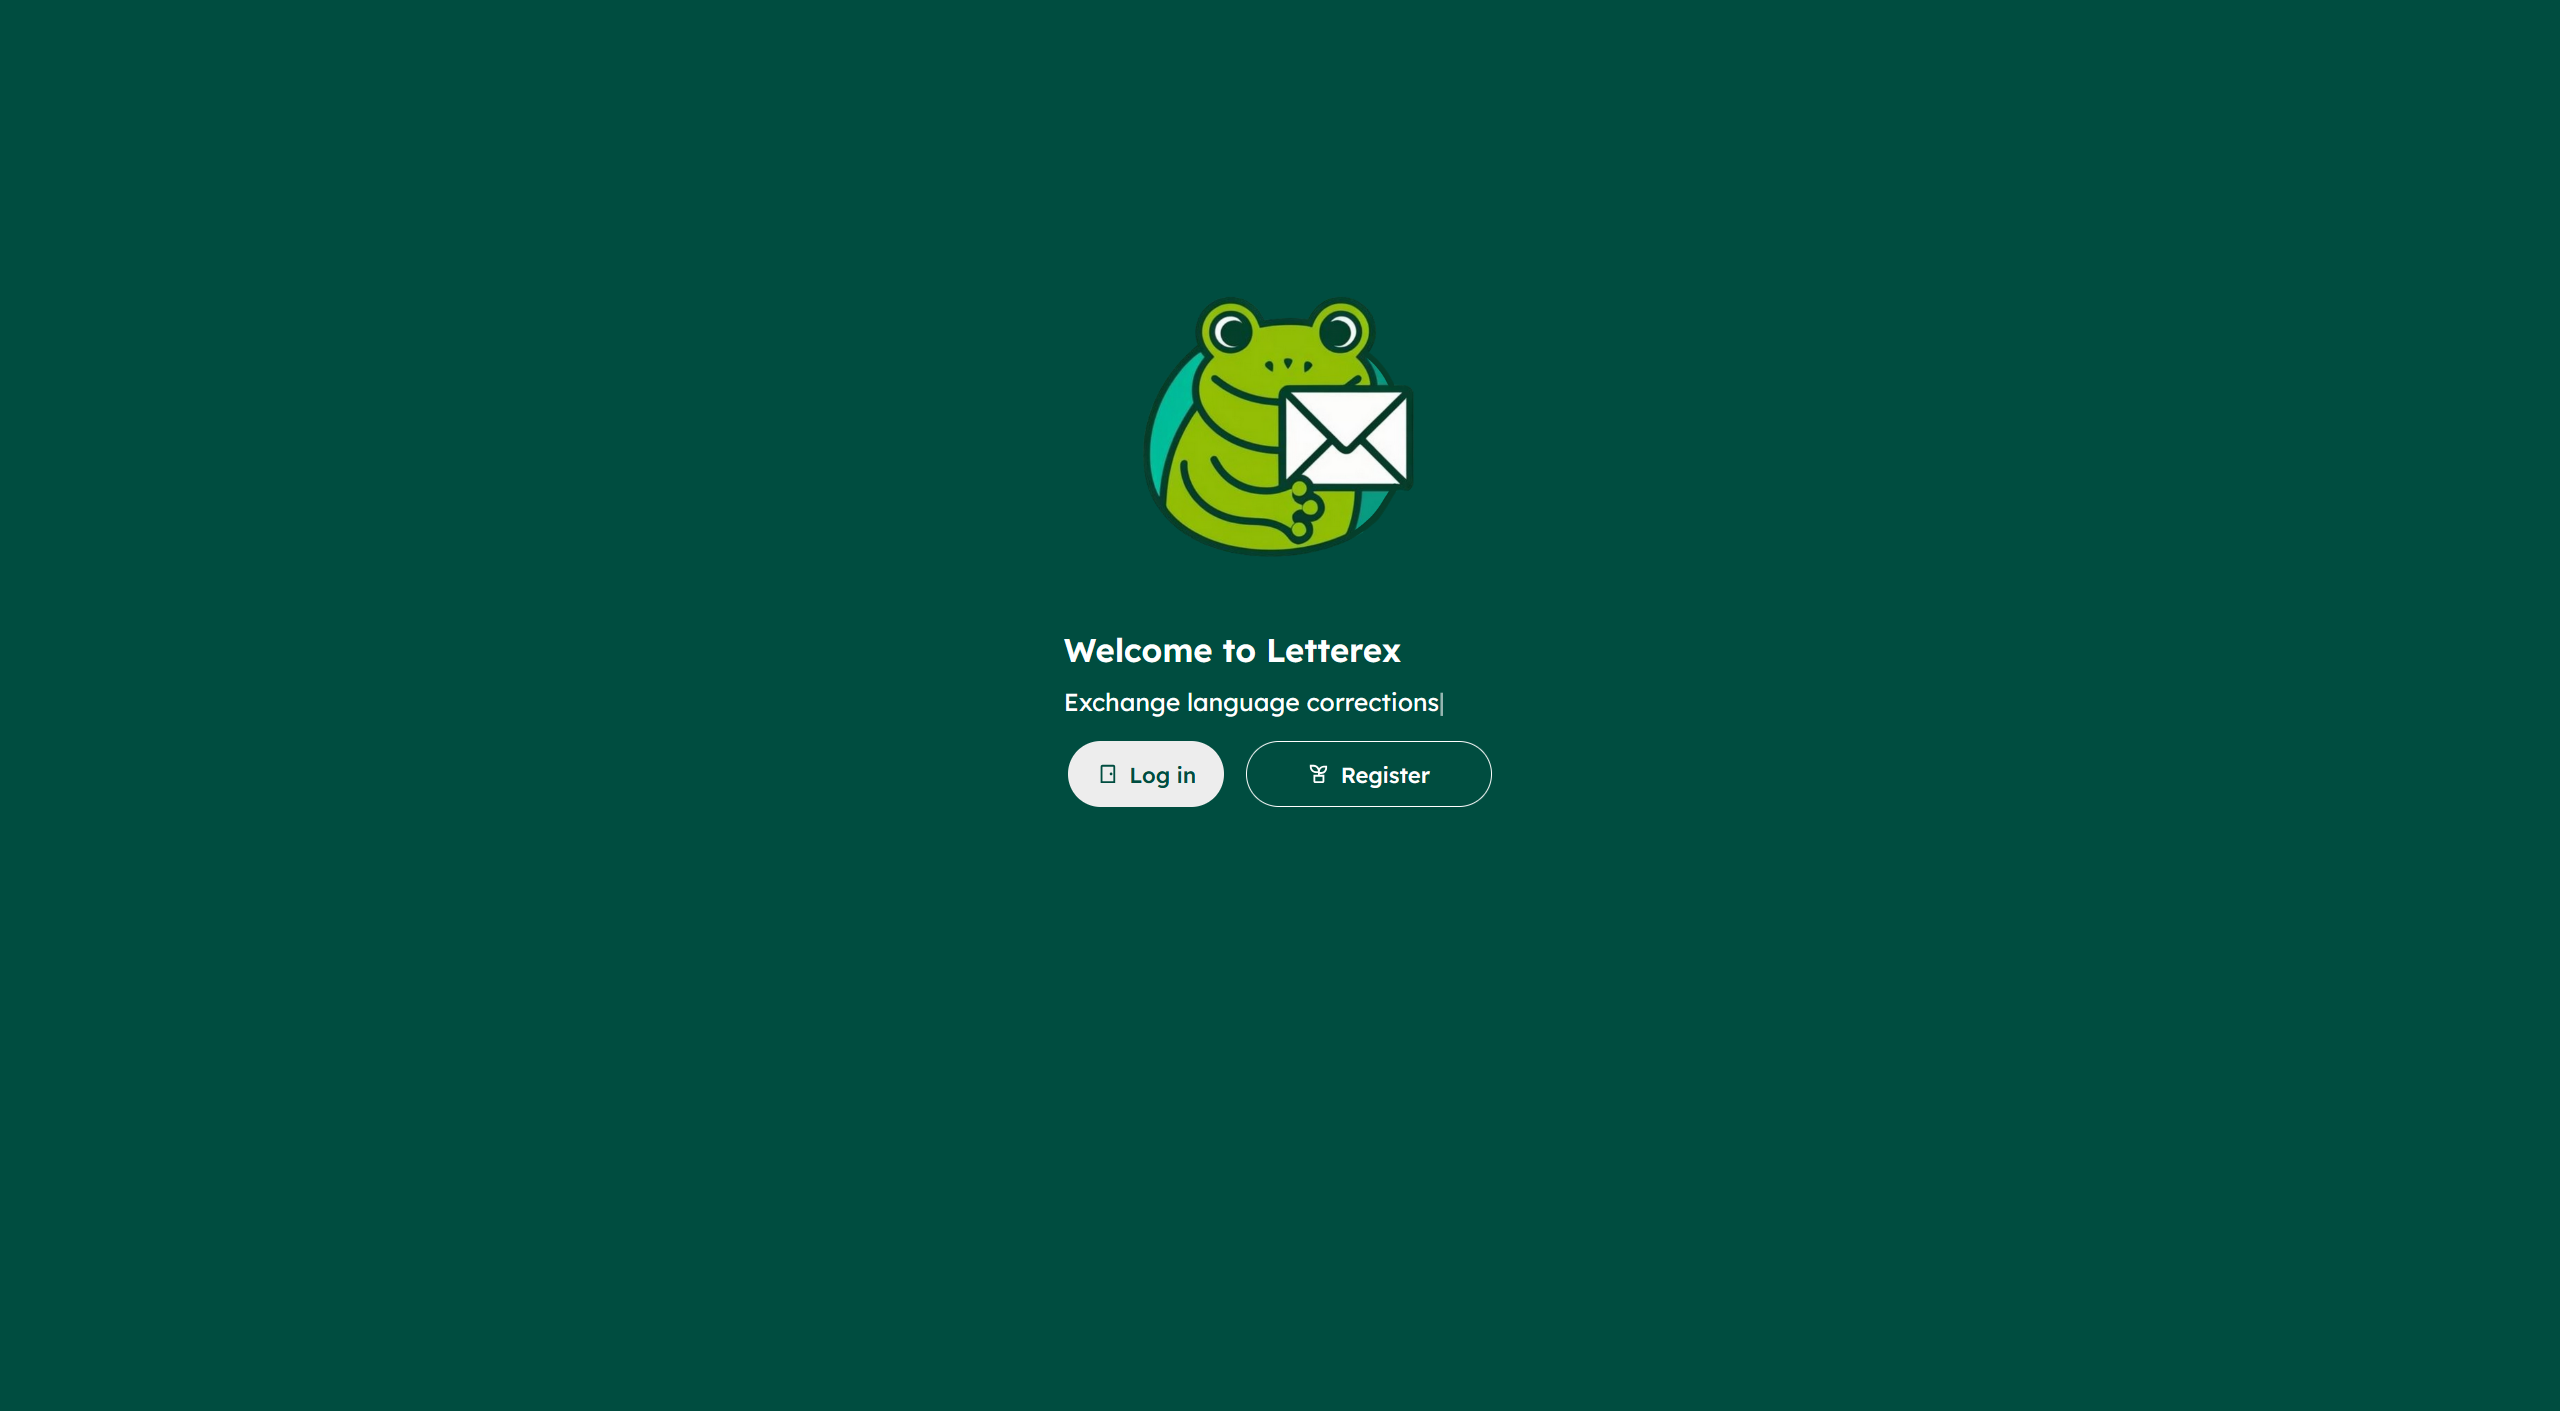
\includegraphics[width=\textwidth]{imagenes/ui/login.png}
    \caption{Página de inicio de sesión y registro}
    \label{fig:landing}
\end{figure}

La página de inicio presenta una interfaz atractiva y animada que da la bienvenida a los usuarios. Esta página utiliza el componente \texttt{AnimatedForm} que gestiona tres estados principales:

\begin{itemize}
    \item \textbf{Bienvenida}: Presenta el propósito de la aplicación con un efecto de escritura animado (\textit{typewriter}) que muestra frases como ``Write about your passions'', ``Exchange language corrections'' y ``Find people to share and learn'', para dar una idea general de aquello en que consiste la plataforma.
    \item \textbf{Inicio de sesión}: Formulario de inicio de sesión para usuarios existentes.
    \item \textbf{Registro}: Formulario de registro con verificación de email mediante el código enviado a su correo, selección de idioma nativo e idiomas de interés, selección de contraseña y nombre de usuario, y posibilidad de subir una foto de perfil.
    \item \textbf{Olvido de contraseña}: Formulario que permite resetear la contraseña del usuario mediante el código de verificación enviado a su email.
\end{itemize}

Una característica distintiva de esta página es la animación del logo implementada con Framer Motion, que se desplaza suavemente entre diferentes posiciones según el formulario activo, proporcionando un elemento lúdico y memorable a la experiencia del usuario.
\subsubsection{Página Principal}

\begin{figure}[h]
    \centering
    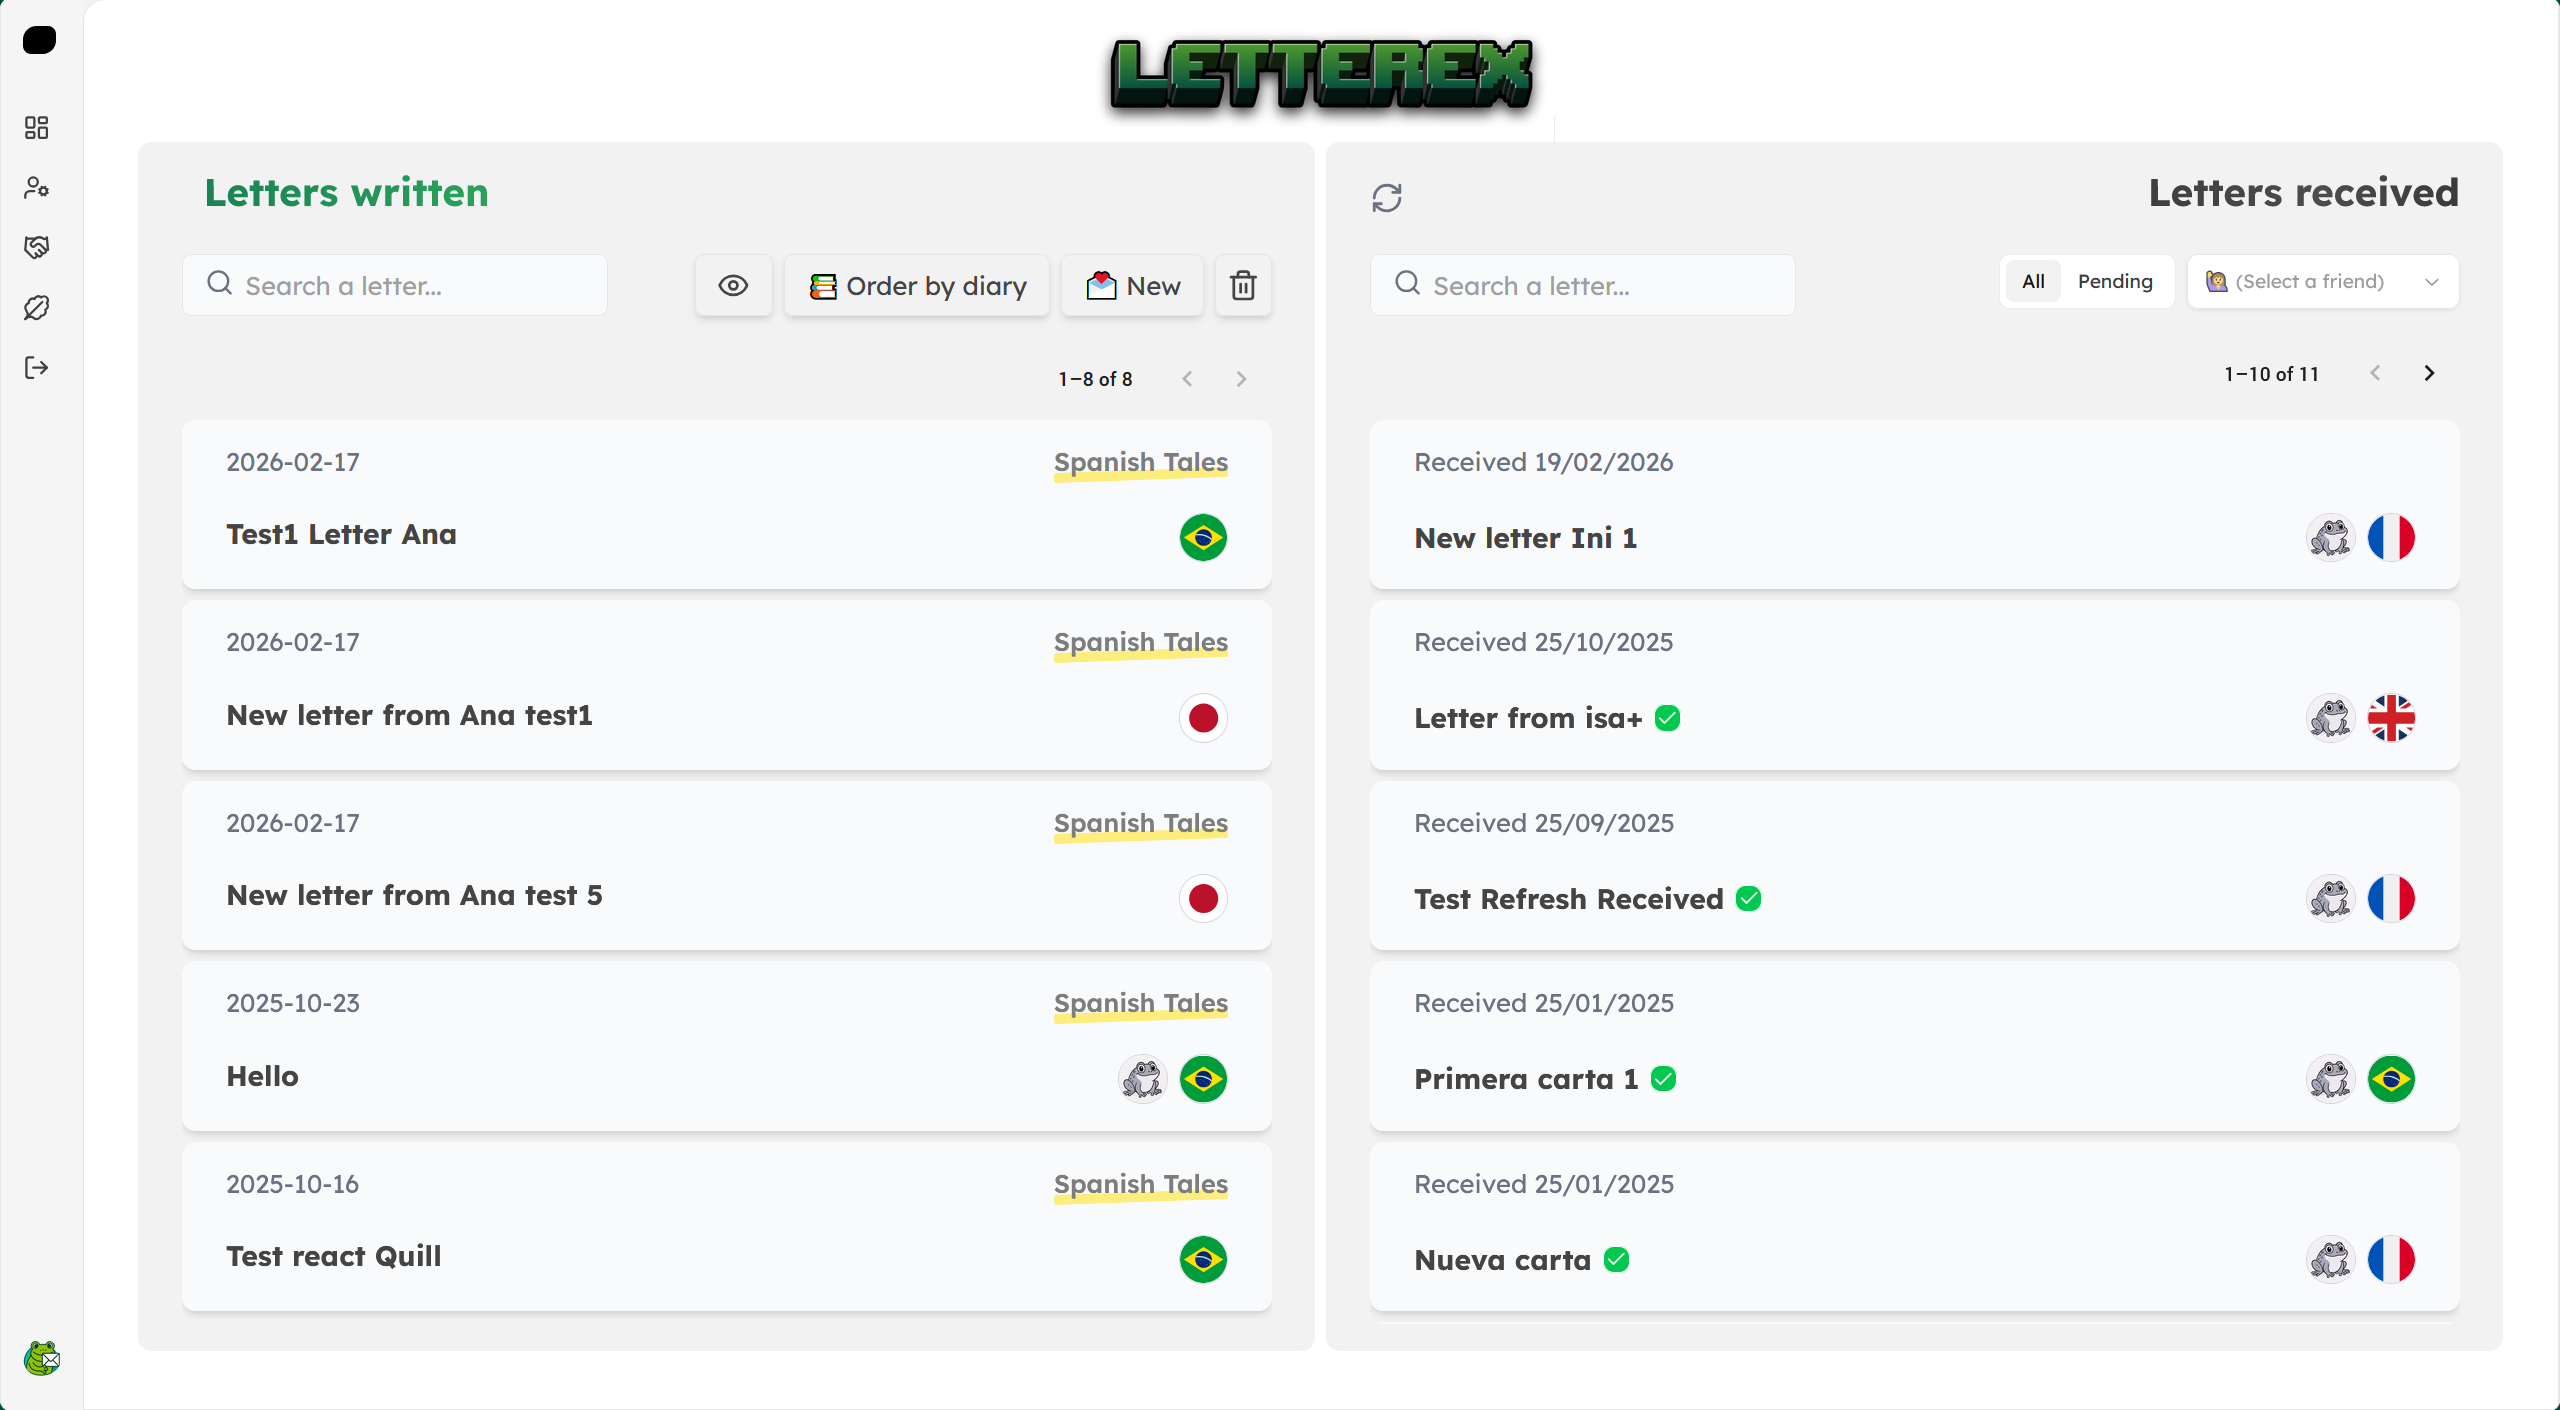
\includegraphics[width=\textwidth]{imagenes/ui/homepage.png}
    \caption{Página principal}
    \label{fig:homepage}
\end{figure}

El dashboard principal (\texttt{/homepage}) es la página central de la aplicación después del inicio de sesión. Está estructurado en dos secciones principales:

\begin{enumerate}
    \item \textbf{Letters Written}: Muestra las cartas que el usuario ha escrito, organizadas en tarjetas interactivas con un efecto de desliz que revela información adicional al interactuar, y paginadas en tandas de 5 elementos. Permite filtrar por una búsqueda, ordenar las cartas por diarios, y eliminar una o varias cartas de la lista. Clicando en la tarjeta de una carta se accede a la página de visualización o edición de esta, clicando en la tarjeta de usuario corrector que aparece al \textit{hover} (posar el cursor sobre el elemento) se accede a la página de visualización de corrección en caso de haberla, y clicando en el botón \textit{New} de la barra de herramientas se accede a la página para crear una nueva carta.
    \item \textbf{Letters Received}: Presenta las cartas recibidas de usuarios que solicitan una corrección por parte del usuario actual, paginadas de la misma forma que las anteriores. Permite filtrar por una búsqueda, por usuario que envió la carta, y por si esa carta está pendiente de corregir (no fue corregida y enviada de vuelta todavía). Clicando en la tarjeta de una carta recibida, se accede a la página de correción de dicha carta.
\end{enumerate}

\subsubsection{Páginas de Creación y Edición de Cartas}

\begin{figure}[h]
    \centering
    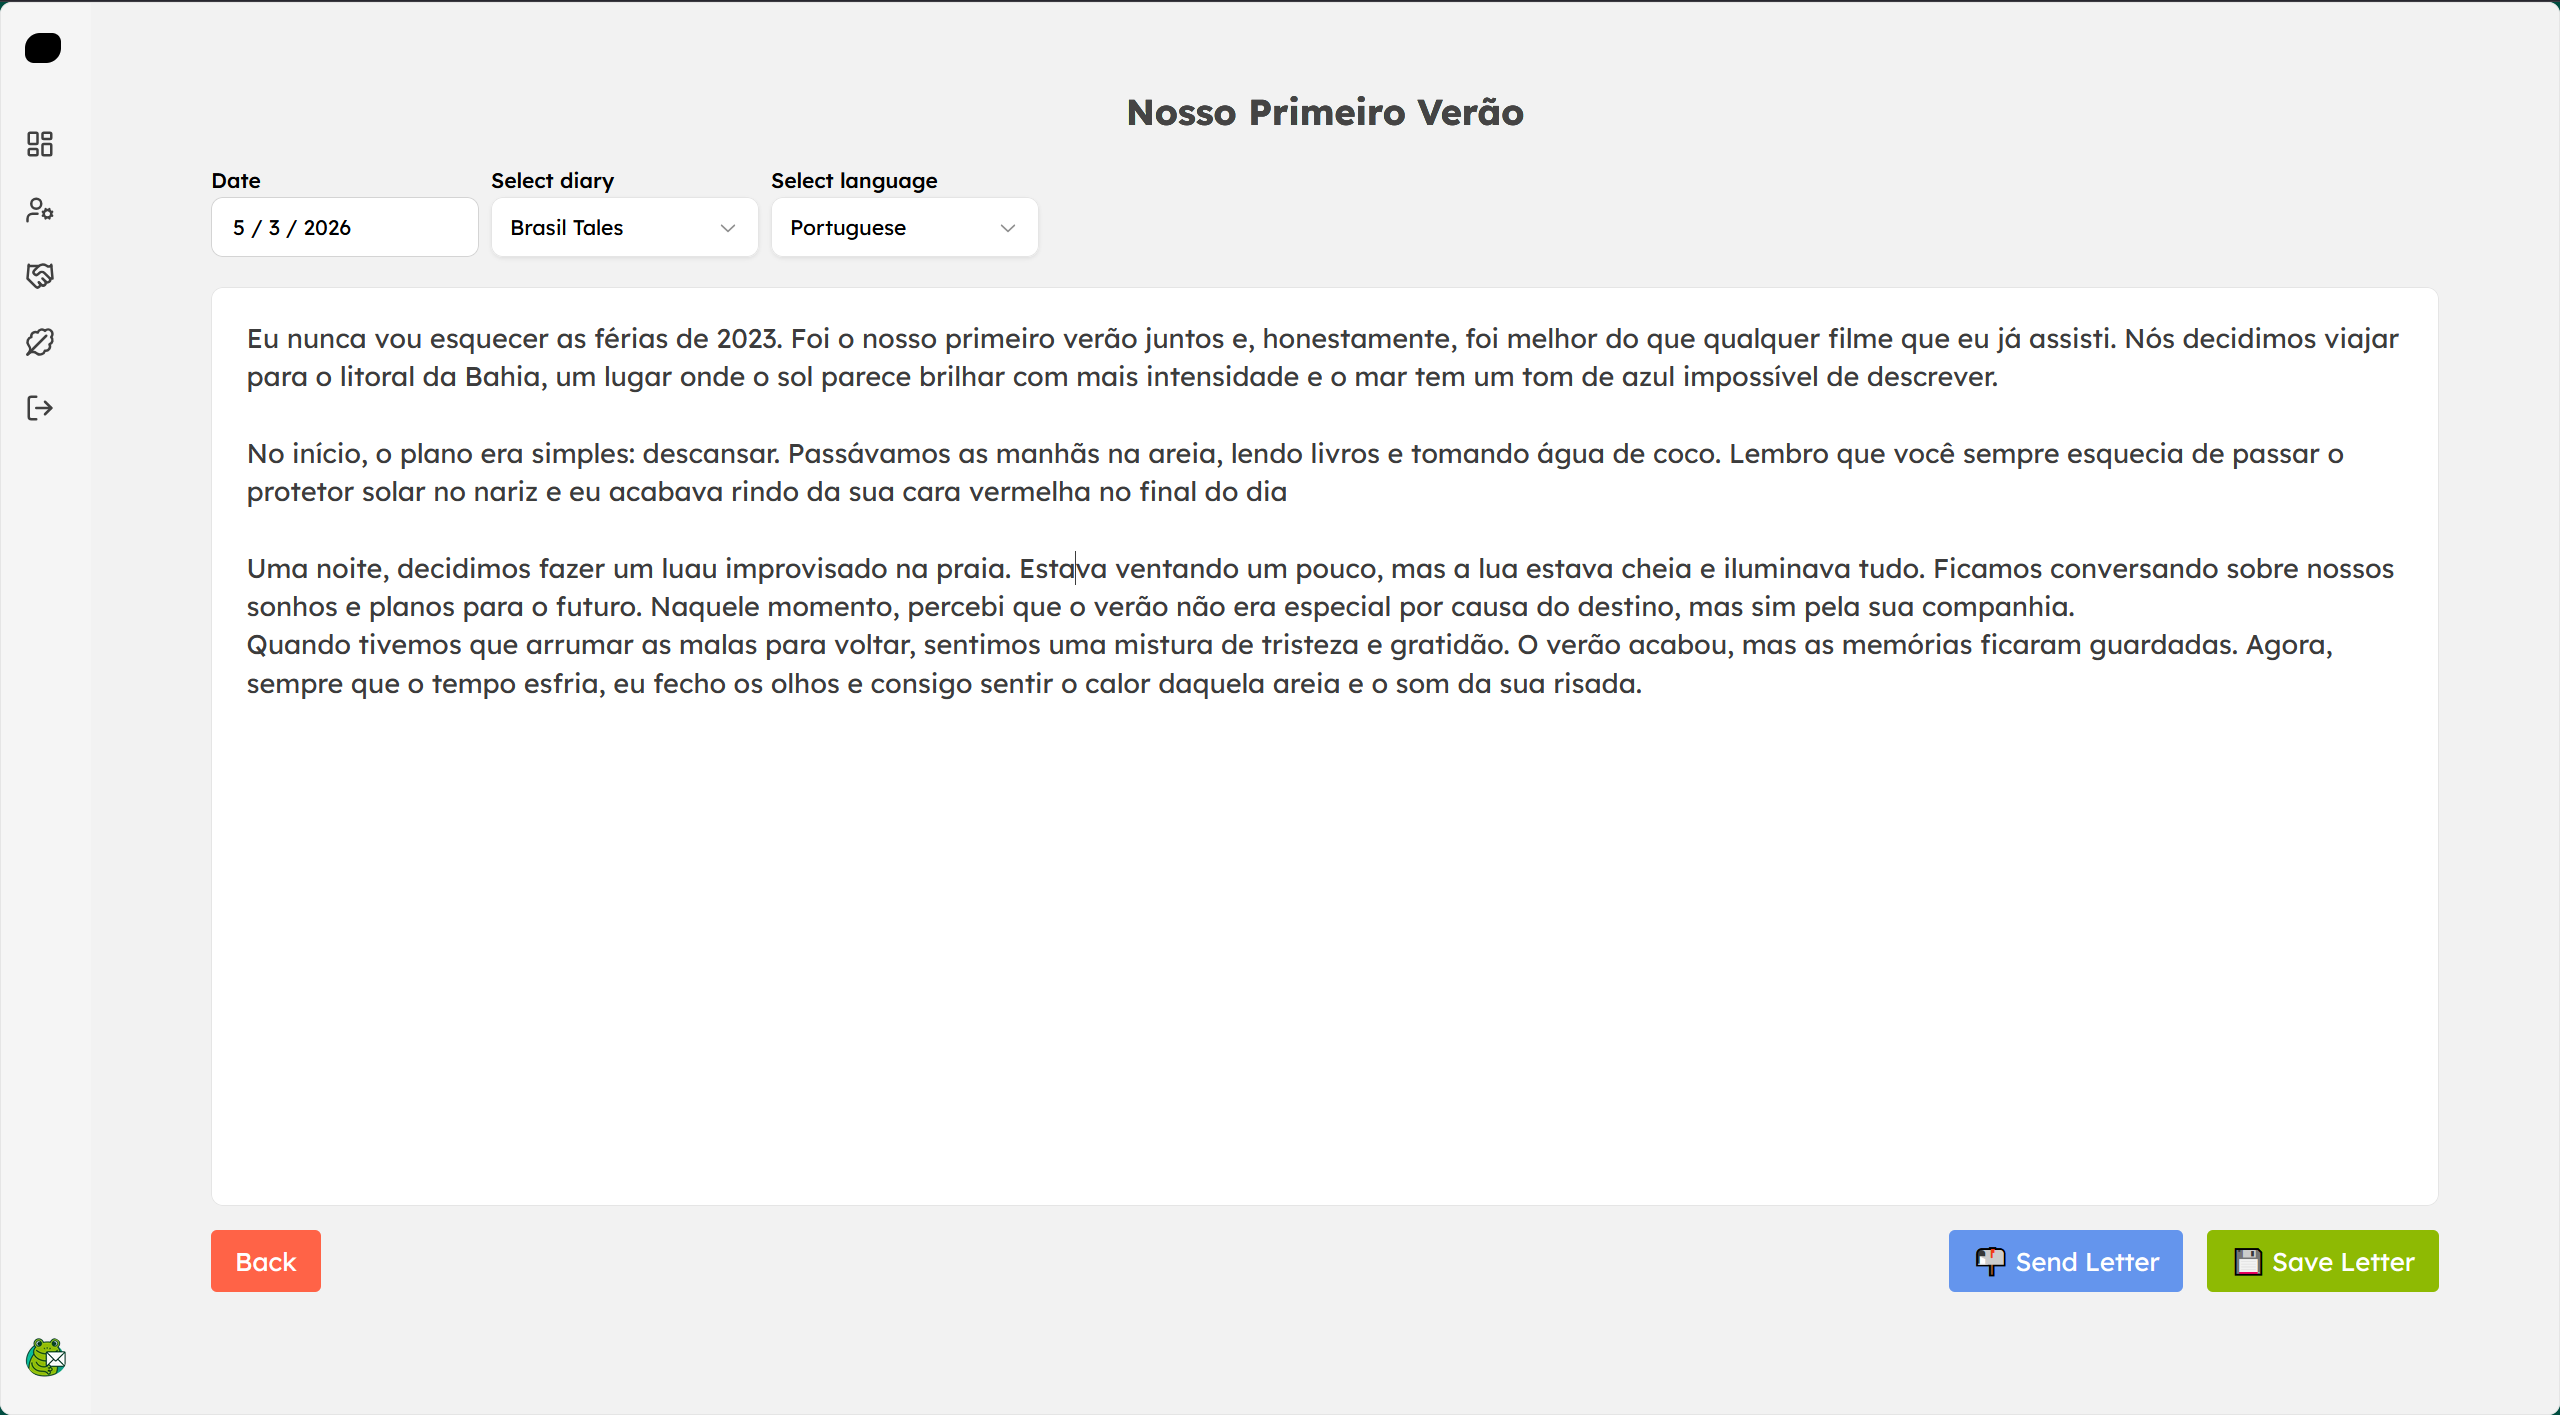
\includegraphics[width=\textwidth]{imagenes/ui/new-letter.png}
    \caption{Página de creación de cartas}
    \label{fig:new-letter}
\end{figure}

La página de creación de cartas (\texttt{/new-letter}) proporciona una interfaz completa para escribir nuevas entradas de diario. El componente implementa validación en tiempo real de los campos requeridos, mostrando mensajes de error específicos cuando el usuario intenta guardar sin completar todos los campos obligatorios. Los elementos principales incluyen campo de título, selectores de fecha, idioma y diario; y un editor de texto enriquecido implementado con React Quill, permite formatear texto con negrita, cursiva, listas, enlaces, etc.\cite{quill_react_playground}

Al guardar la carta, se redirige al usuario a una página muy similar (\texttt{/edit-letter}), lo que permite el guardado de borradores de forma que se pueda seguir editando la carta en otro momento. Esta última página es muy similar a la de Creación de Cartas, salvo que en ella es posible enviar la carta a amigos para que la corrigan.

\subsubsection{Página de Corrección de Cartas}

\begin{figure}[h]
    \centering
    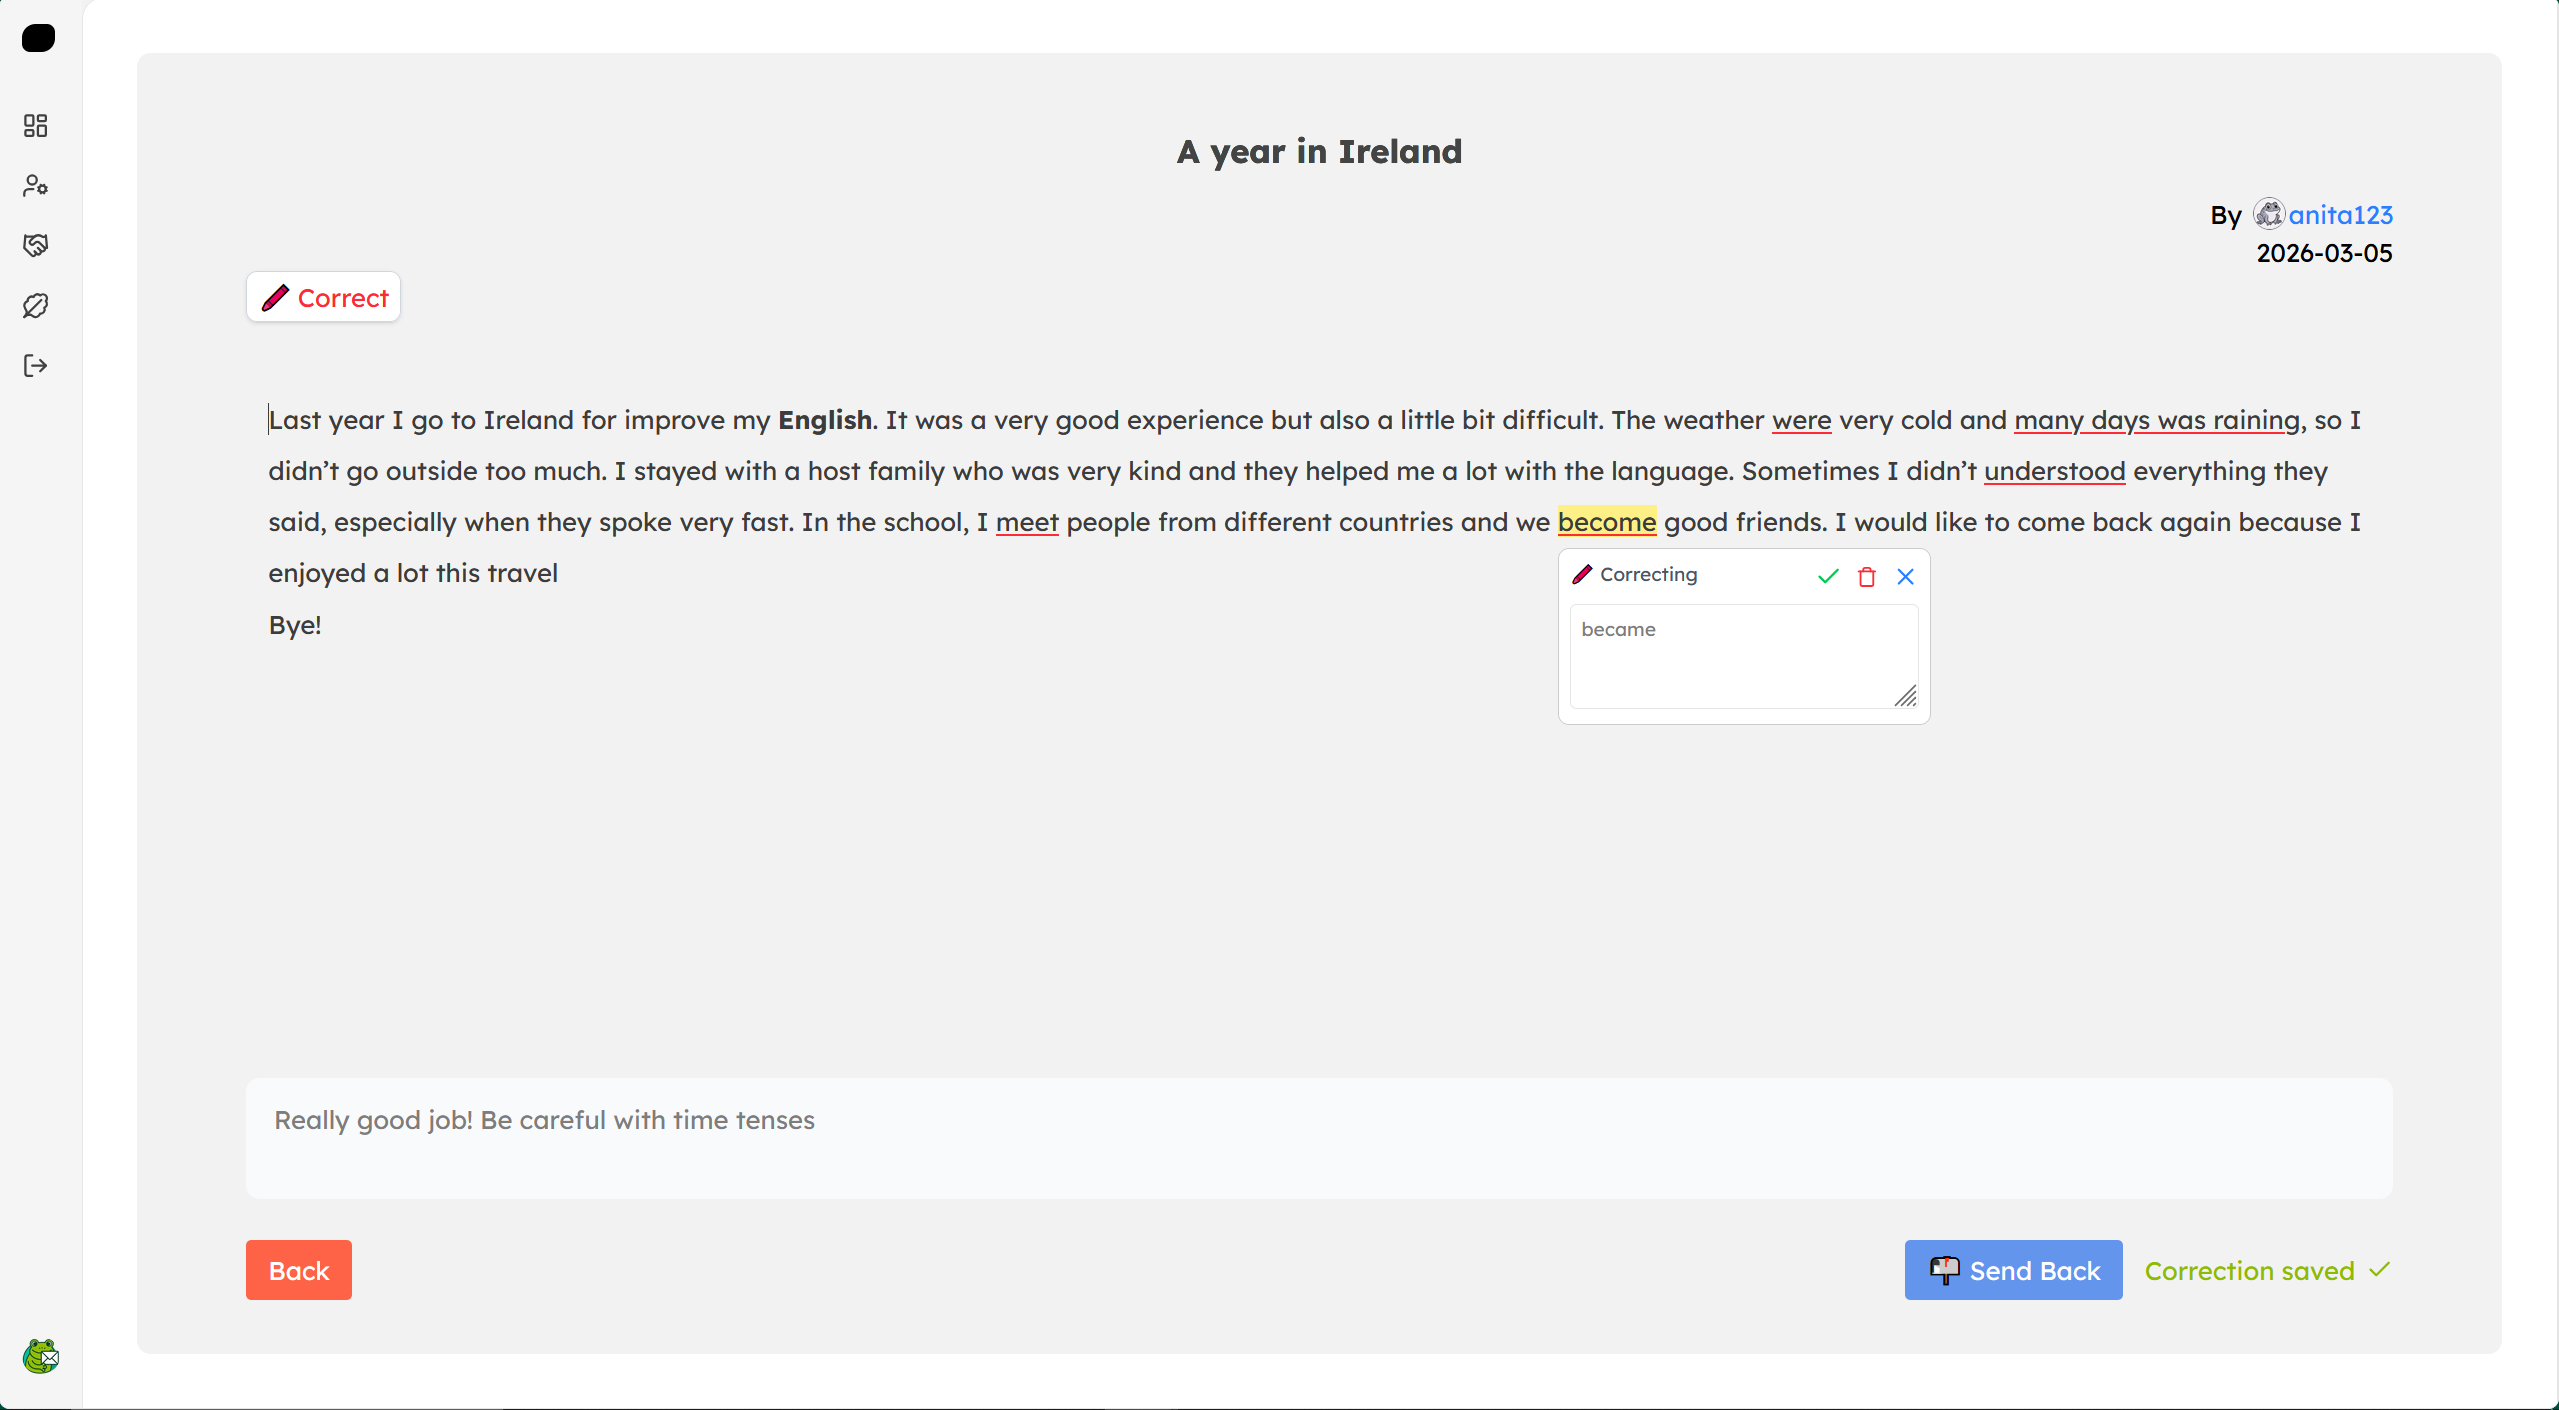
\includegraphics[width=\textwidth]{imagenes/ui/correct-letter2.png}
    \caption{Página de corrección de cartas}
    \label{fig:correct-letter}
\end{figure}

Esta página (\texttt{/correct-letter}) permite a los usuarios corregir las cartas escritas por otros en idiomas que dominan.

Para añadir correcciones, el usuario debe seleccionar fragmentos específicos del texto original que considere que contienen errores o se puede matizar. El texto seleccionado se resalta visualmente, y se abre un panel de escritura para asociarlo con una corrección sugerida o un comentario explicativo. Además de las correcciones específicas, el corrector puede dejar un comentario general sobre la carta al final.

El componente \texttt{TextCorrections} renderiza de forma dinámica el texto con las correcciones aplicadas. El proceso incluye:

\begin{enumerate}
    \item Parseo del texto original: Se divide el texto en fragmentos según las posiciones de corrección.
    \item Detección de solapamientos: Antes de añadir una nueva corrección, se verifica que no se solape con correcciones existentes mediante comparación de índices.
    \item Renderizado diferenciado: Cada fragmento se renderiza con estilos diferentes según sea texto sin corregir o texto corregido. Concretamente, el texto corregido va marcado en amarillo al hover y subrayado en rojo.
    \item Interactividad: Los fragmentos corregidos son interactivos. Al clicar en ellos o pasar el cursor, se abre un panel donde se pueden añadir o editar las correcciones.
\end{enumerate}

Para hacer esto posible, esta es la estructura de datos que se asocia a una corrección:

\begin{center}
\begin{minipage}{0.36\textwidth}
\begin{verbatim}
interface Correction {
    id: string;
    startIndex: number;
    endIndex: number;
    originalText: string;
    correctedText: string;
}
\end{verbatim}
\end{minipage}
\end{center}

\subsubsection{Página de Visualización de Correcciones Recibidas}

\begin{figure}[h]
    \centering
    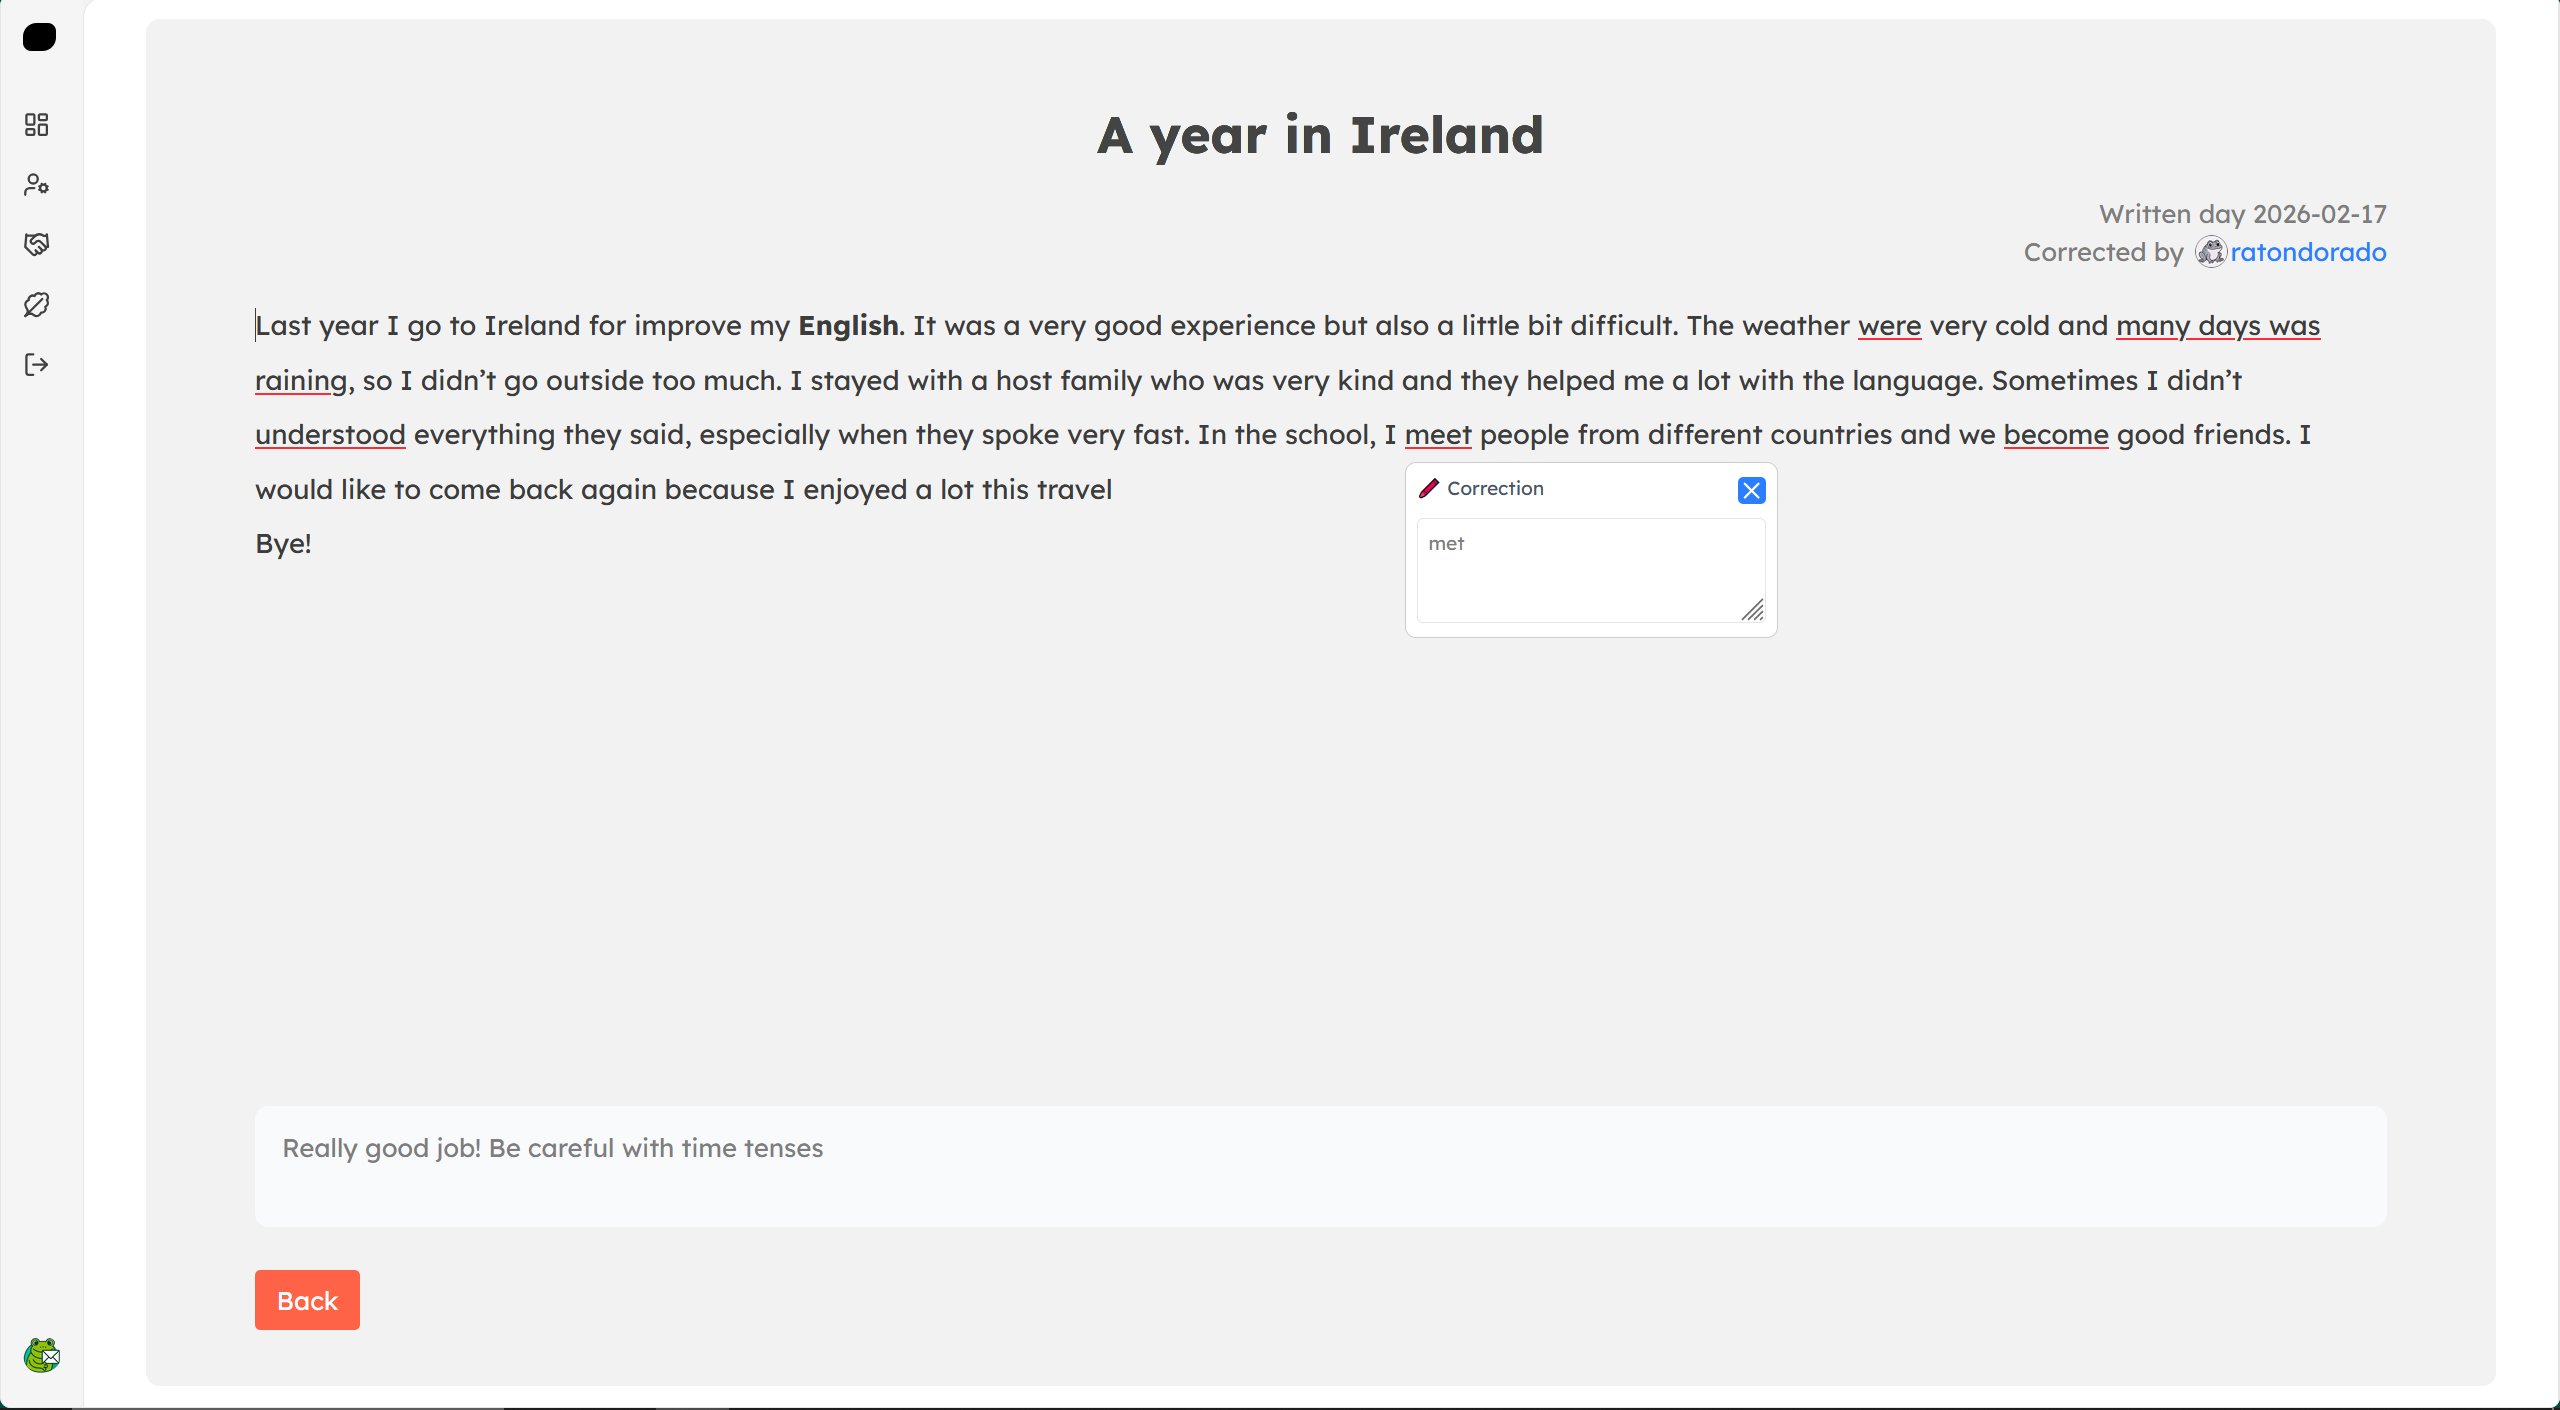
\includegraphics[width=\textwidth]{imagenes/ui/view-correction.png}
    \caption{Página de visualización de corrección recibida}
    \label{fig:view-correction}
\end{figure}

La página de visualización (\texttt{/view-correction}) de correcciones presenta al usuario remitente las correcciones recibidas en sus cartas. Esta interfaz permite al usuario aprender de sus errores de forma efectiva, clara y visualmente agradable. La interfaz es similar a la de Corrección de Cartas, pero sin permitir editar o enviar la corrección.

Se muestra el texto original con las secciones corregidas resaltadas en color diferenciado. Al hacer click o hover sobre una sección corregida, se muestra un panel con la corrección sugerida. Se muestran también los comentarios generales del corrector sobre la carta, y la información del corrector (nombre e imagen de perfil), que actúa como enlace a su página de perfil.

\subsubsection{Página de Amigos}

\begin{figure}[h]
    \centering
    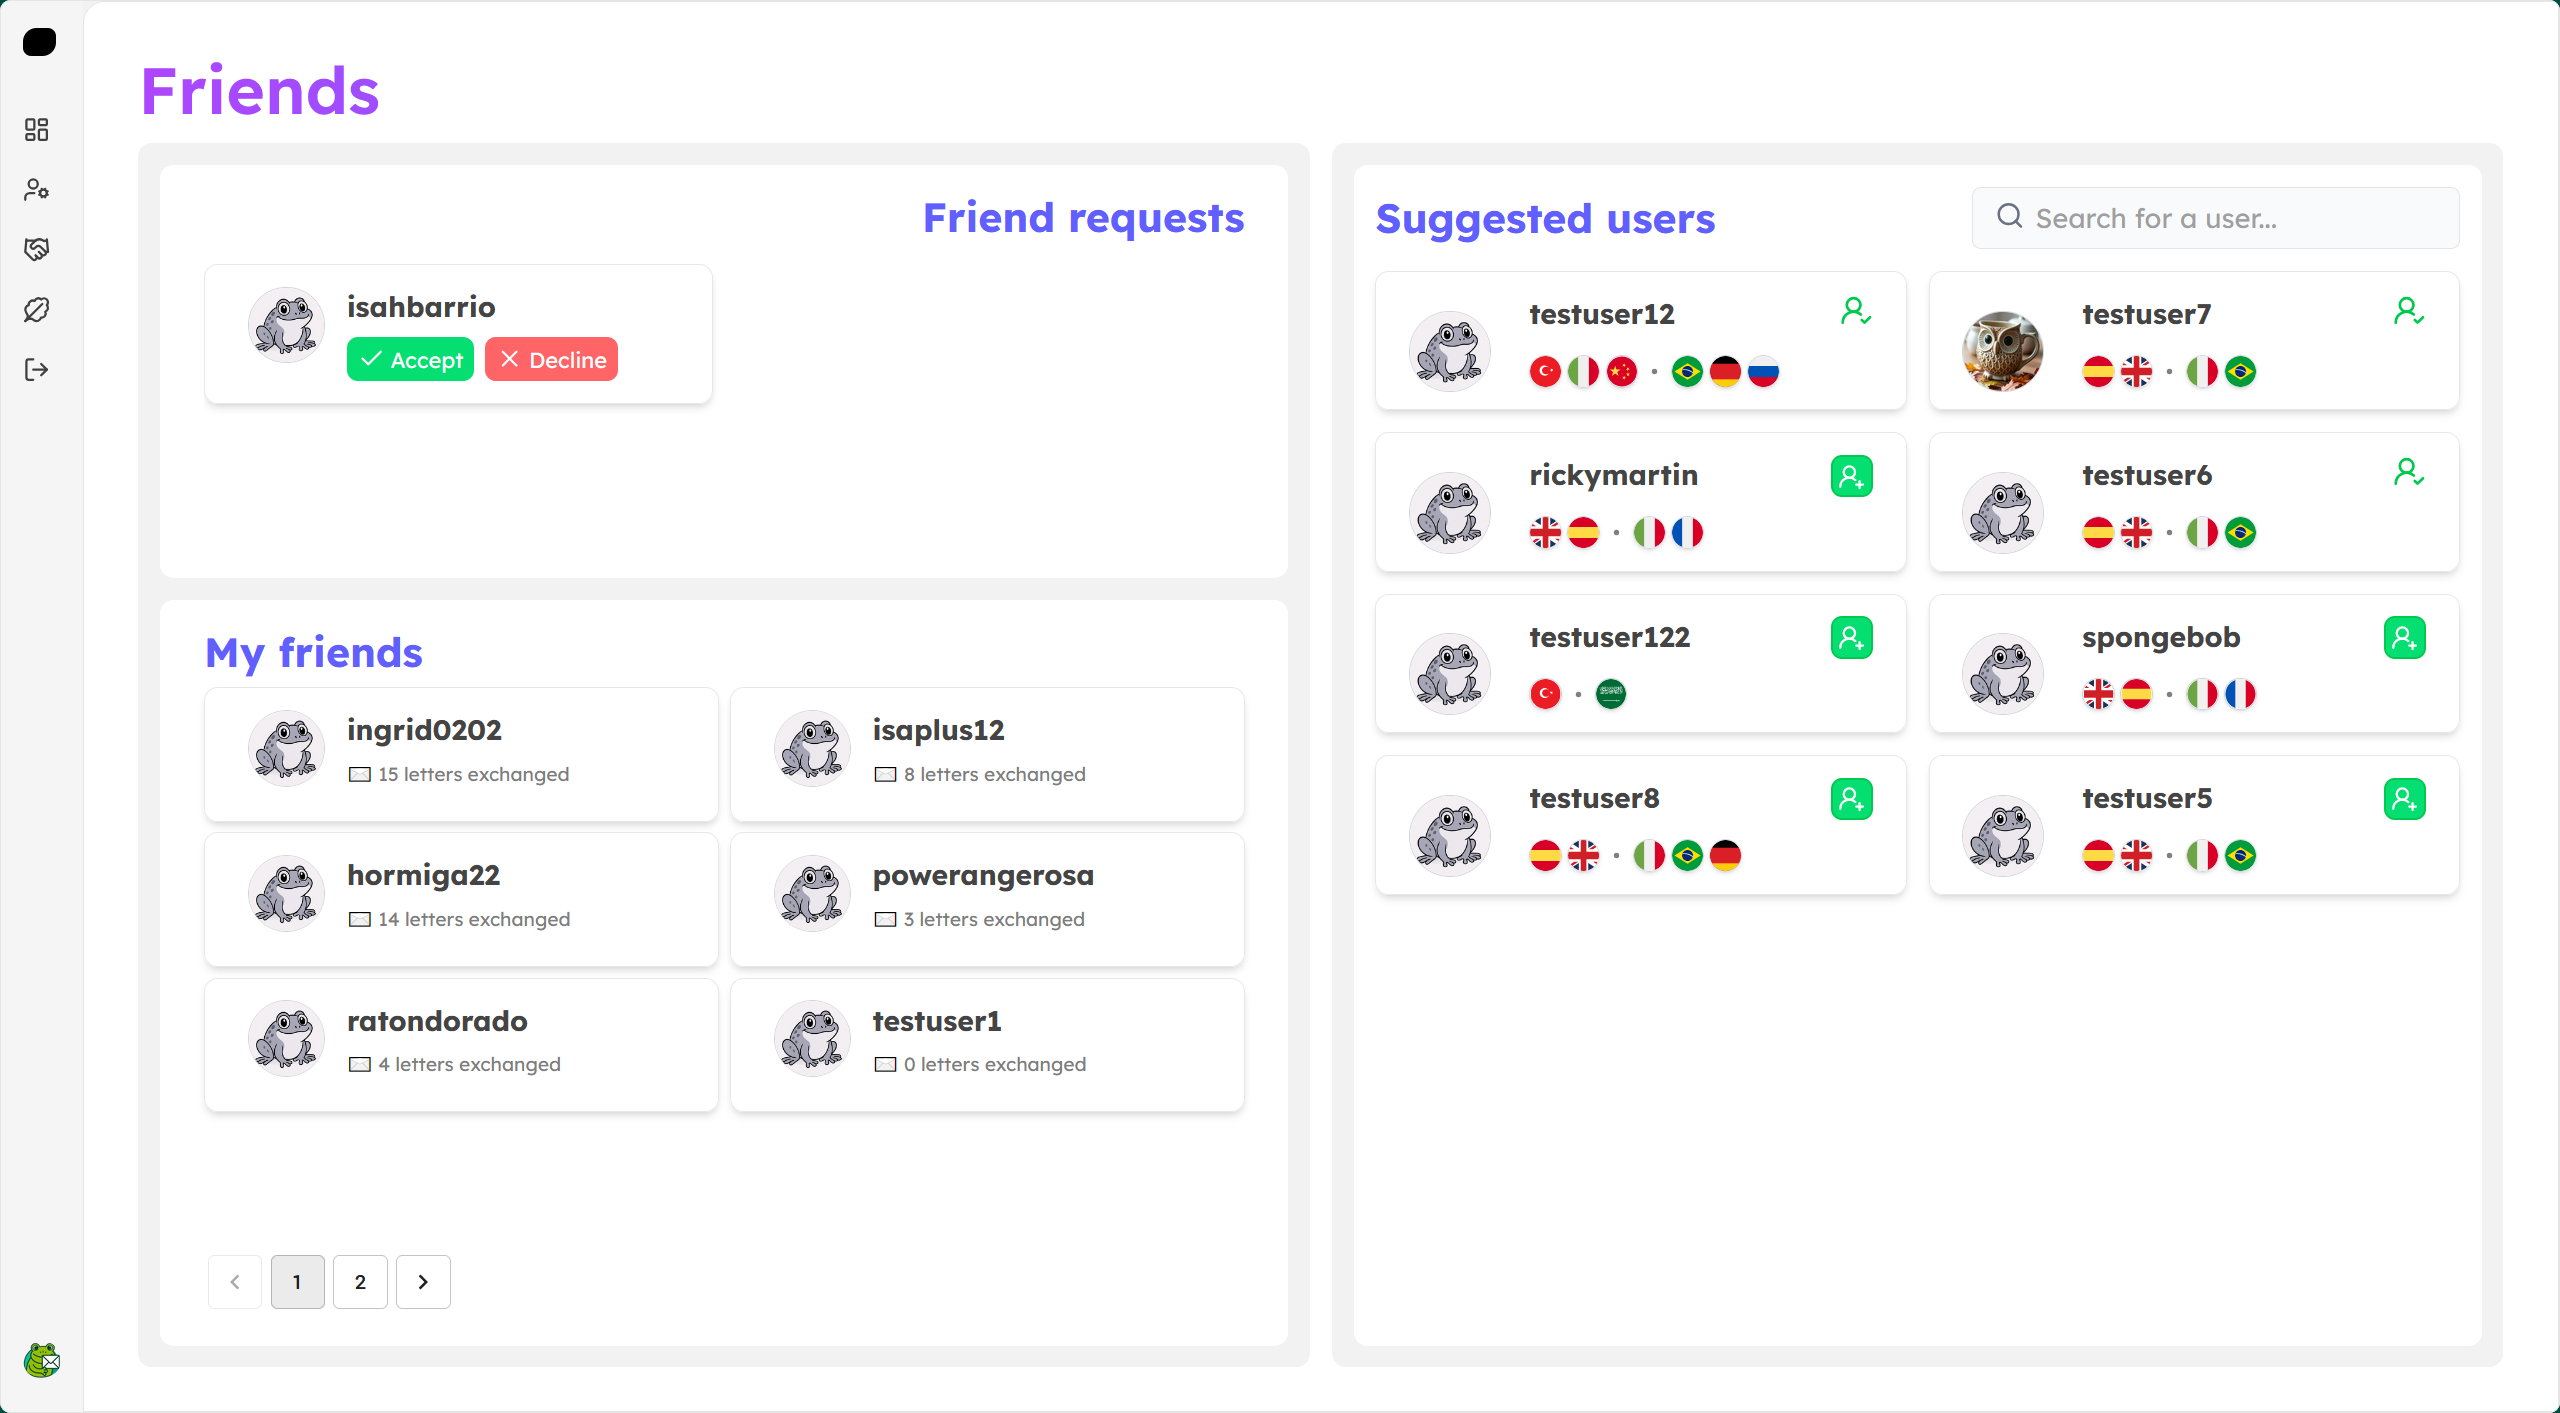
\includegraphics[width=\textwidth]{imagenes/ui/friends-page.png}
    \caption{Página de amigos}
    \label{fig:friends}
\end{figure}

En la página de amigos (\texttt{/friends}), el usuario puede gestionar las relaciones sociales dentro de la aplicación. Se divide en tres secciones:

\begin{enumerate}
    \item \textbf{Solicitudes de amistad}: Muestra las solicitudes pendientes recibidas, con opciones para aceptar o rechazar.
    \item \textbf{Lista de amigos}: Presenta las amistades establecidas con su avatar, nombre y estadísticas como el número de cartas intercambiadas.
    \item \textbf{Usuarios sugeridos}: Muestra usuarios recomendados basándose en idiomas en común, además de un buscador por nombre de usuario para poder encontrar un usuario en concreto que se desee agregar.
\end{enumerate}

La página implementa paginación para todas estas listas de usuarios y solicitudes. También, al clicar cualquiera de las tarjetas de usuario, se accede a la página de perfil de este.

\subsubsection{Página de Perfil de Usuario}

\begin{figure}[H]
    \centering
    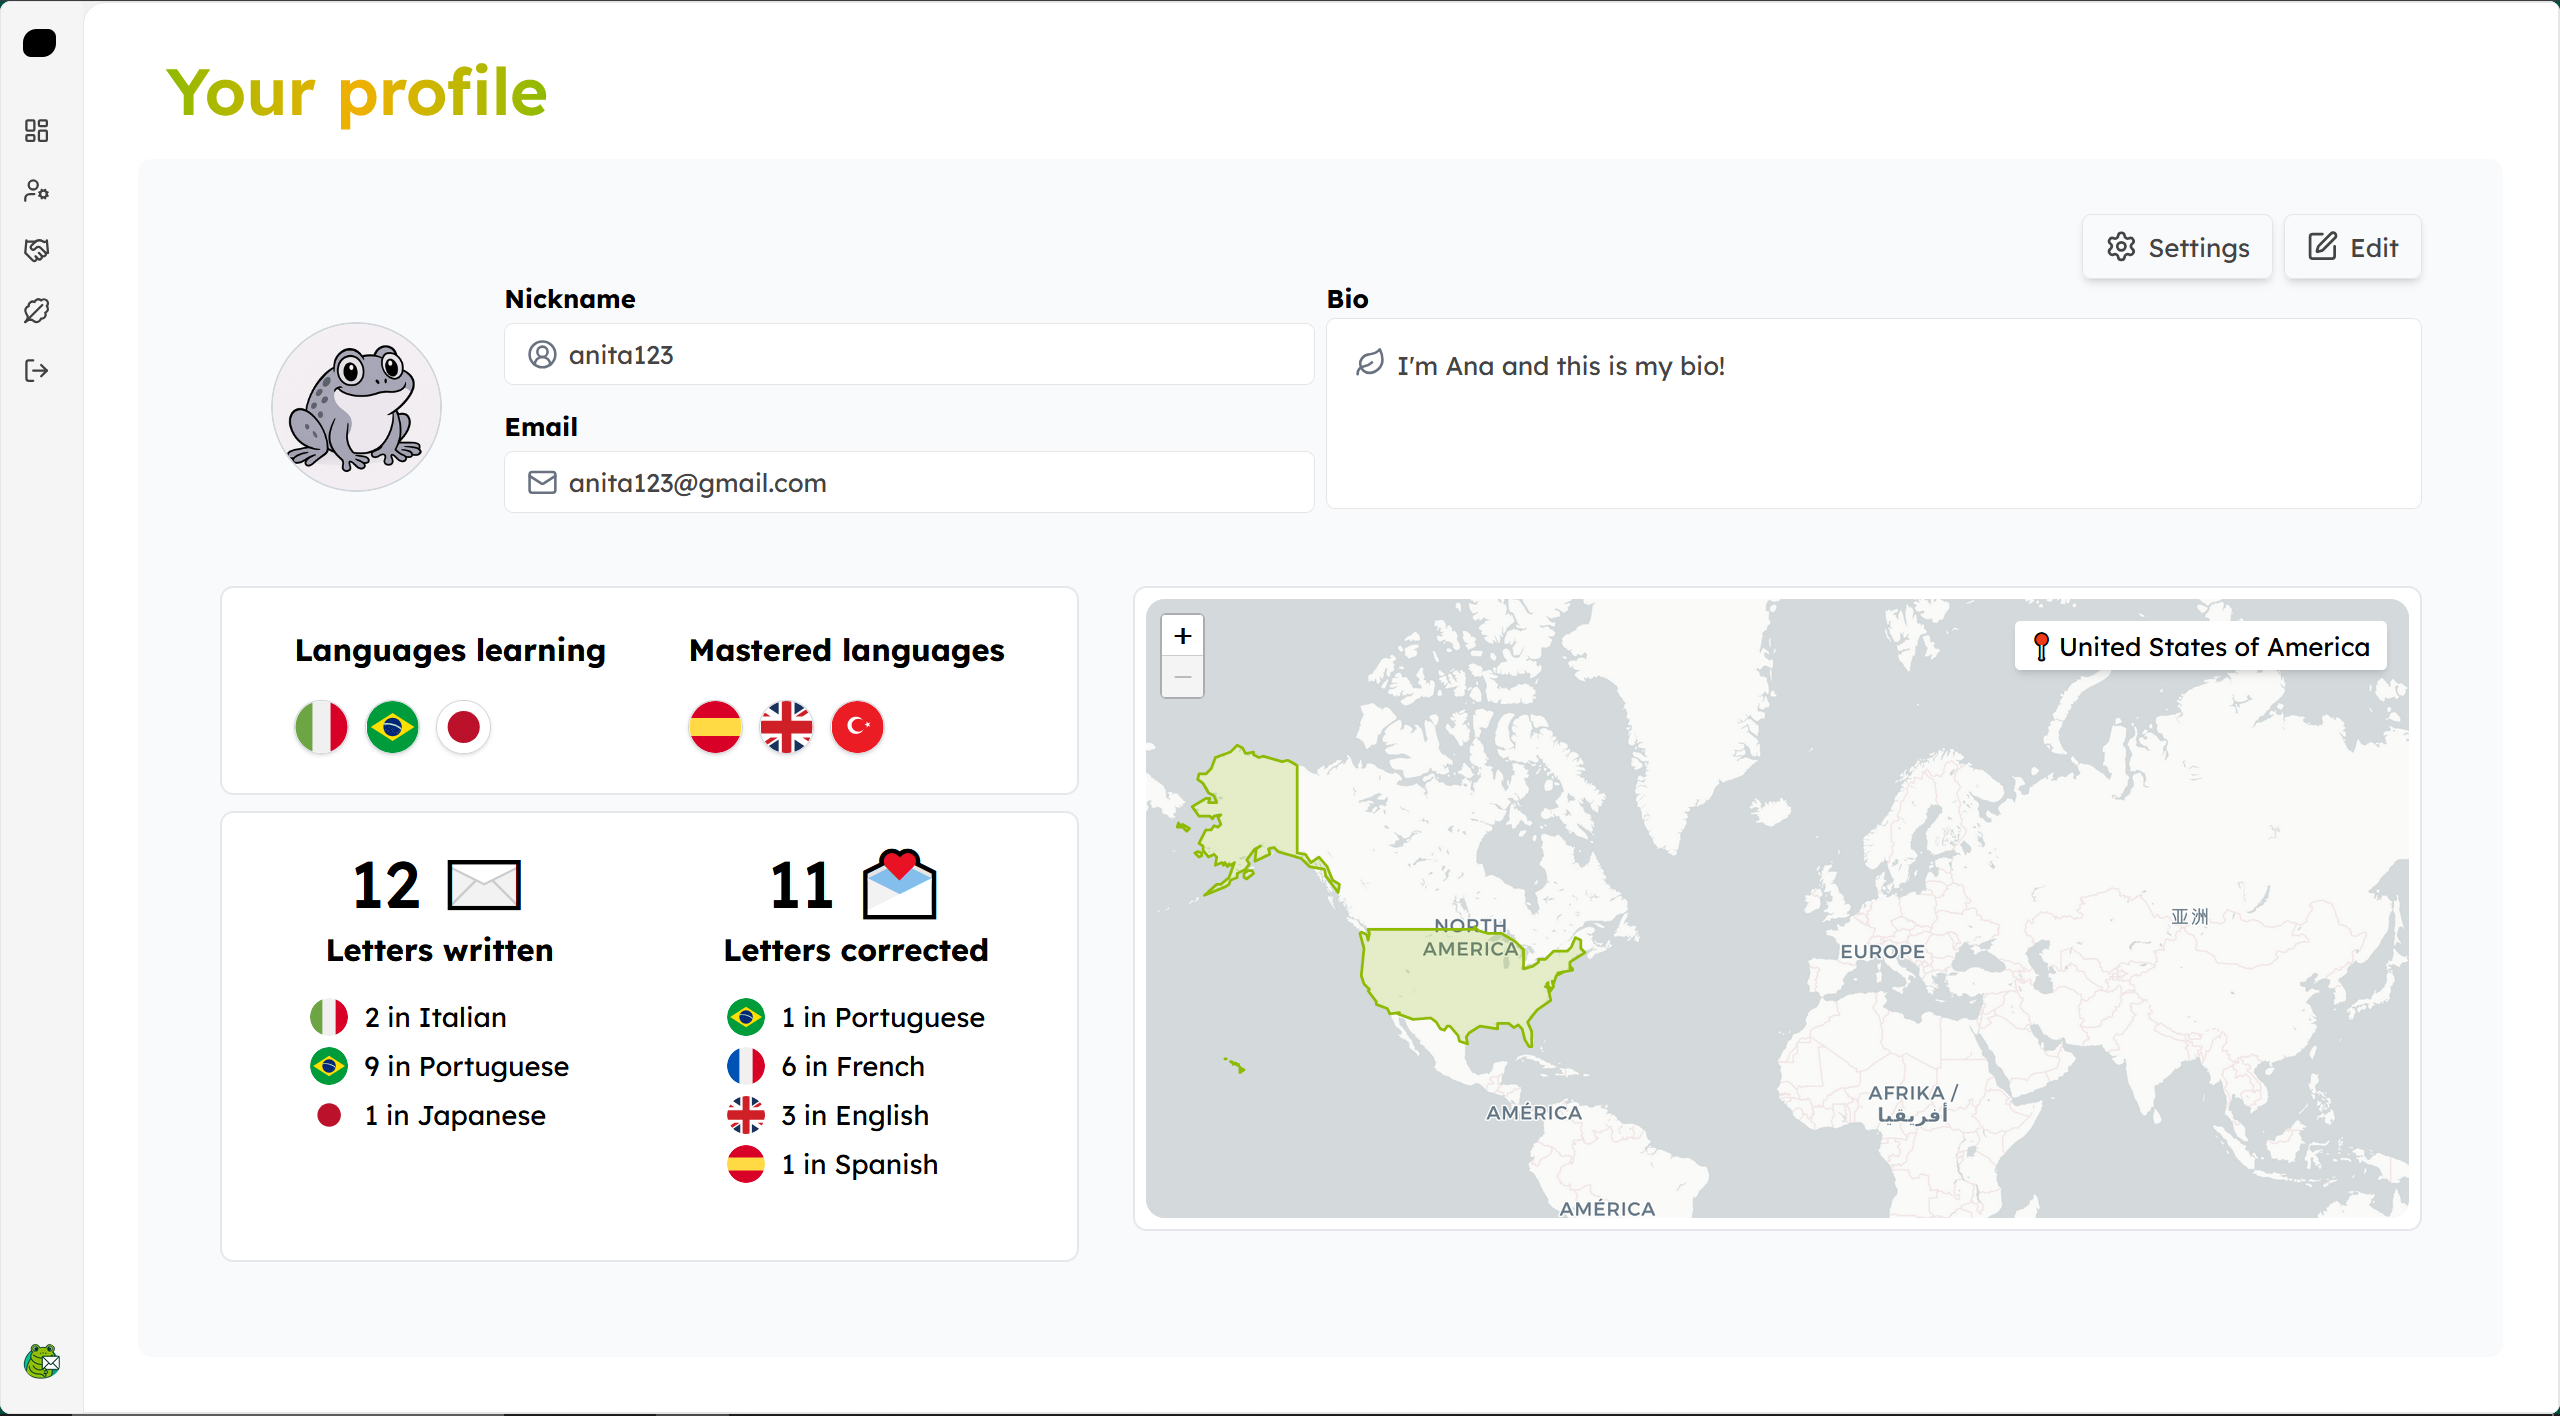
\includegraphics[width=\textwidth]{imagenes/ui/my-profile.png}
    \caption{Página de perfil de usuario}
    \label{fig:profile}
\end{figure}

La página de perfil muestra información detallada sobre un usuario. Se utiliza la misma página para el perfil propio y para el de otros usuarios. La página incluye:

\begin{itemize}[label={-}]
    \item Foto de perfil, nombre y biografía.
    \item Idiomas nativos y lenguas que está aprendiendo.
    \item Estadísticas de cartas escritas y corregidas en cada idioma.
    \item Ubicación geográfica visualizada en un mapa interactivo de React Leaflet.
    \item Para el perfil de usuario ajeno, un botón para dar la opción de eliminar de la lista de amigos en caso de tener a ese usuario agregado.
    \item Para el perfil de usuario autenticado (mi perfil), opciones de edición de la información del perfil y de configuración (cambiar contraseña o eliminar la cuenta).
\end{itemize}

\subsection{Técnicas de Optimización}

Finalmente, al igual que en el backend, en el frontend se han implementado varias técnicas de optimización. Estas técnicas se han aplicado de forma complementaria y selectiva, con el objetivo de mejorar el rendimiento de la aplicación y la experiencia de usuario en distintos niveles: carga de recursos, fluidez de la navegación, renderizado de componentes y comunicación con el backend.

\begin{enumerate}
    \item \textbf{Importaciones Dinámicas}: Componentes pesados como el mapa de la página de perfil se cargan dinámicamente solo cuando son necesarios. Esto es posible gracias a la función \texttt{dynamic} de Next.js, diseñada para optimizar el rendimiento mediante la técnica de carga diferida (\textit{Lazy Loading}) de los componentes, que asegura que el navegador descargue el código de estos componentes no al inicio sino en el momento en que los necesite. Mientras se carga, aparece un mensaje para informar al usuario del estado de carga.
    \begin{verbatim}
        const ImageUploader = dynamic(
            () => import("@/components/imageUploader"),
            { loading: () => <div>Loading...</div> }
        );
    \end{verbatim}

    \item \textbf{Memoización}: En la app se usan las funciones de React \texttt{useCallback} y \texttt{useMemo} para evitar recrear funciones y recalcular datos en cada renderizado.

    \item \textbf{Paginación}: Las listas de registros (cartas, correcciones, amigos) incluyen paginación para reducir la cantidad de datos cargados y renderizados simultáneamente. Se cargarán más elementos del servidor solo cuando el usuario lo solicite pasando de página en la lista.

    \item \textbf{Debouncing}: En campos de búsqueda y filtrado, se implementa debouncing para reducir el número de llamadas a la API, como se ha descrito en la sección anterior de arquitectura del backend.

    \item \textbf{Lazy Loading de imágenes}: Las imágenes de perfil se cargan de forma diferida para mejorar el tiempo de carga inicial.

    \item \textbf{Pantallas esqueleto}: Para mejorar la experiencia del usuario durante la carga de datos, se han utilizado pantallas esqueleto (\textit{skeleton screens}). Se genera una estructura visual gris translúcida que replica la de la página real (títulos, bloques de contenido, botones...) mientras se cargan los datos del servidor. Esto reduce la sensación de espera porque el usuario ya ve dónde aparecerá cada elemento. Una vez que los datos llegan, el esqueleto se reemplaza con el contenido definitivo.

    \begin{figure}[H]
        \centering
        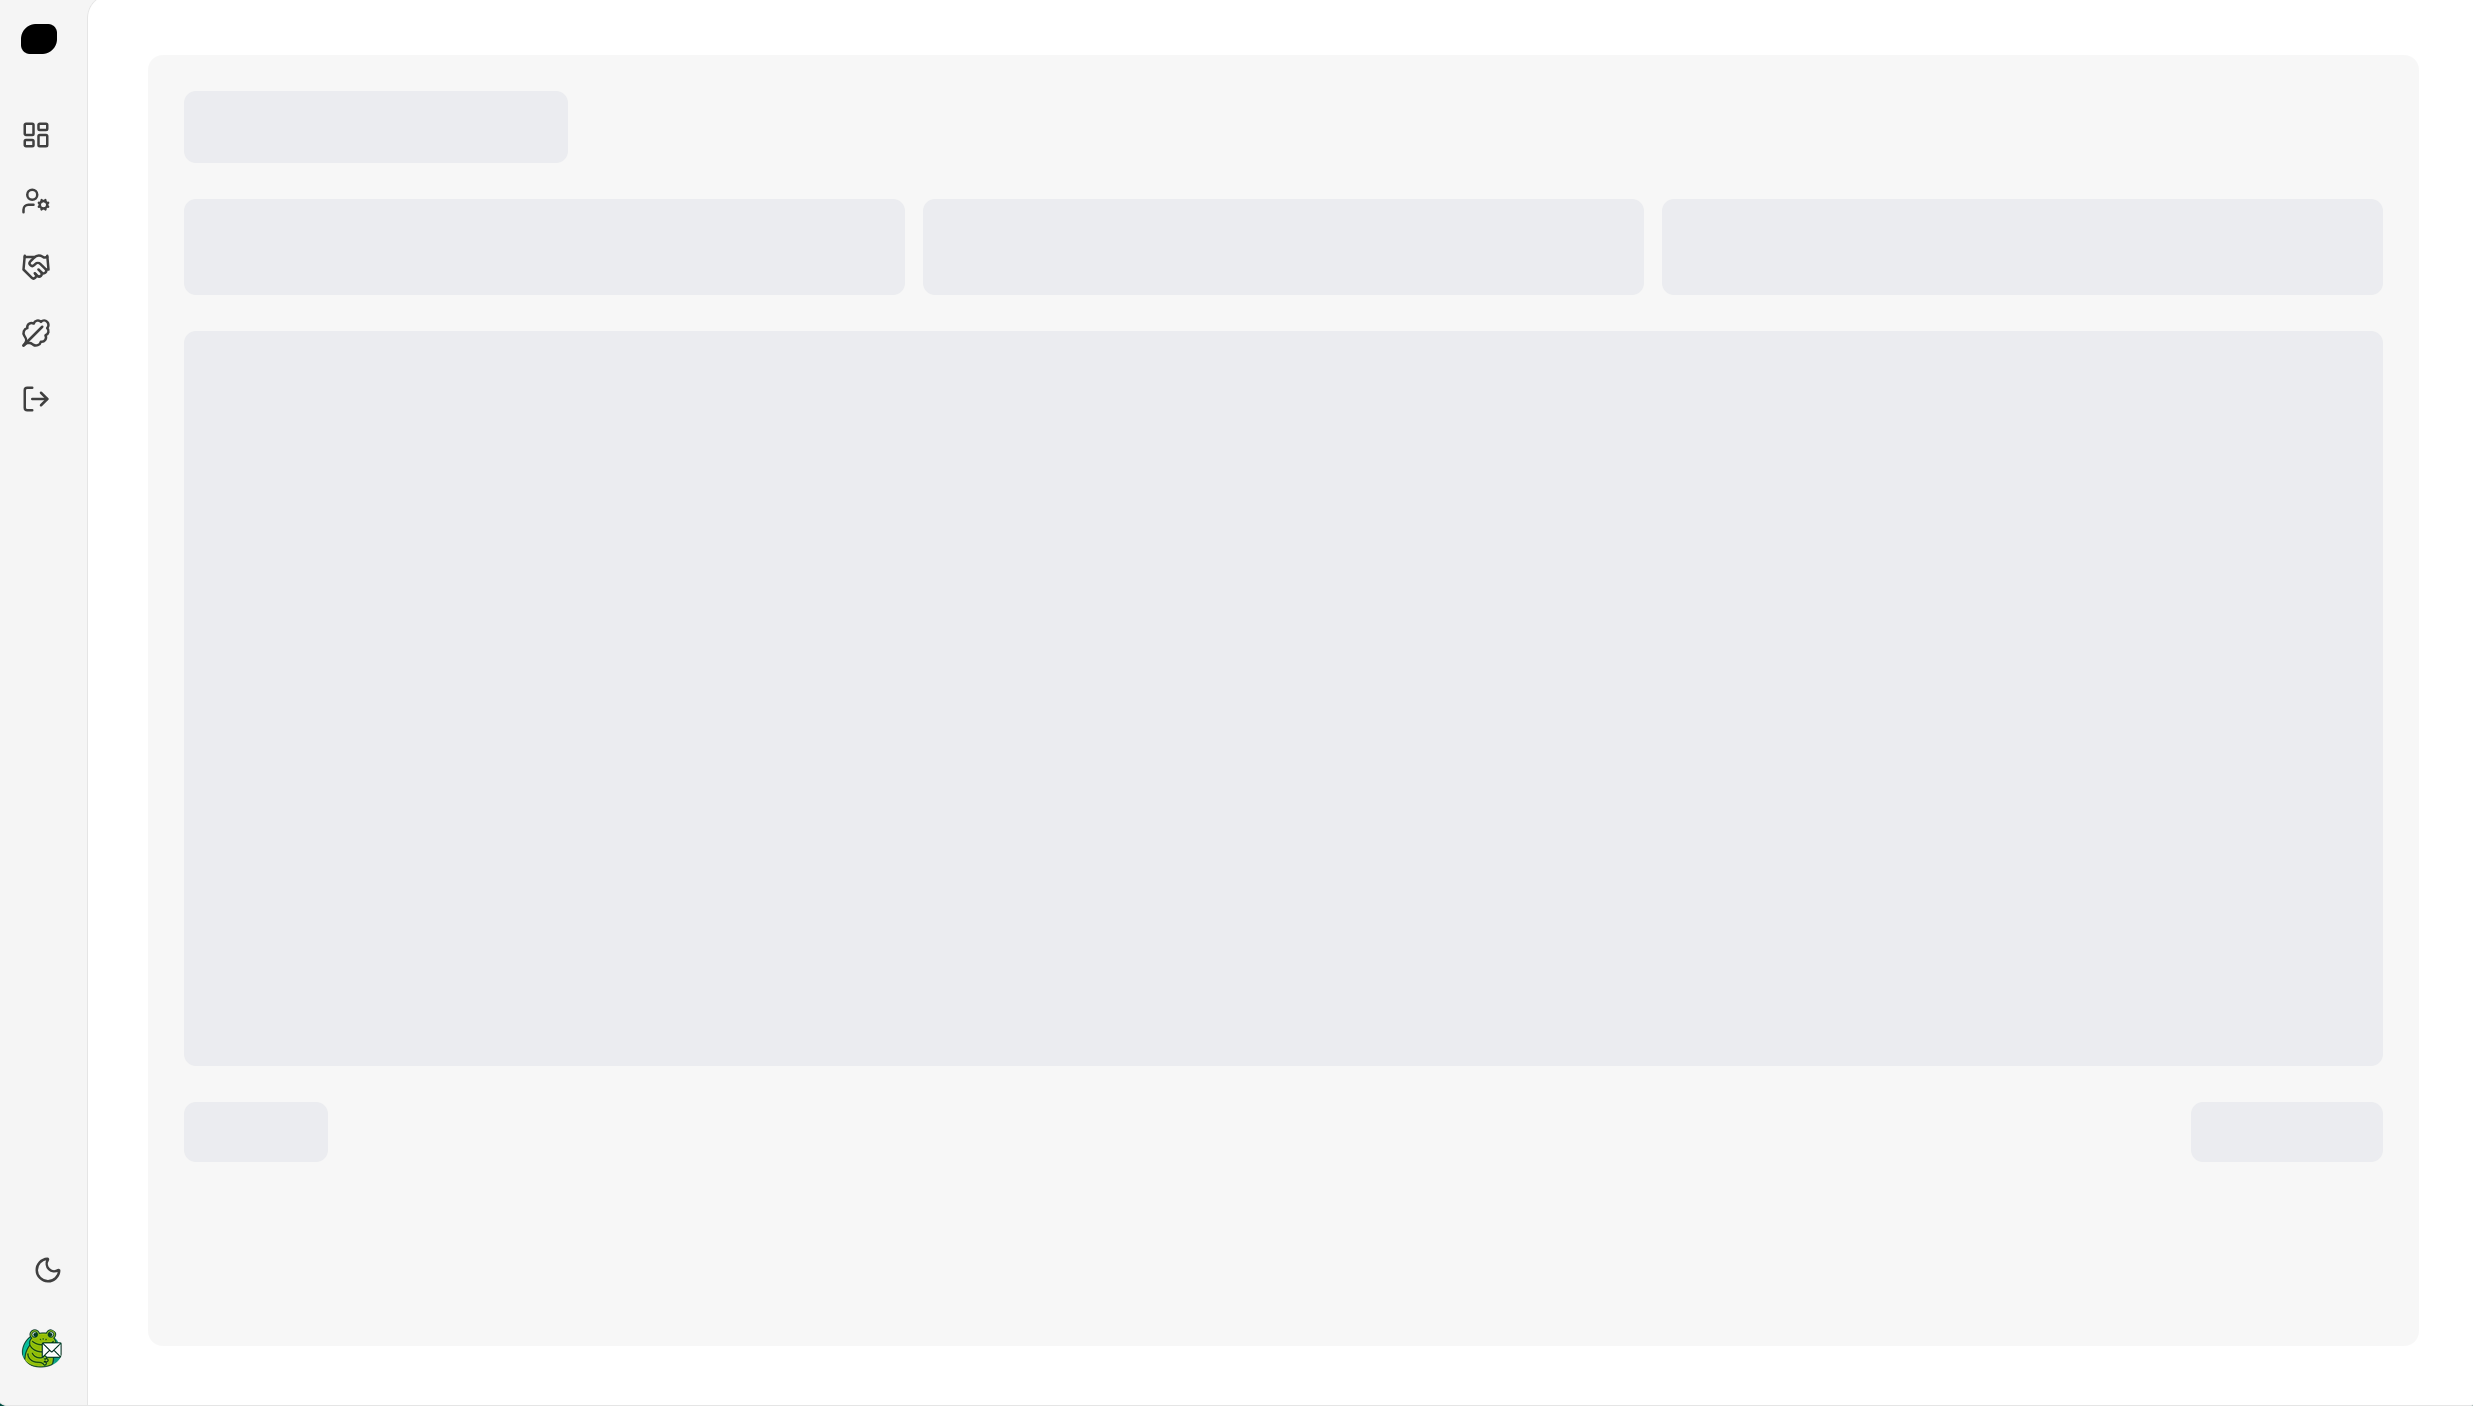
\includegraphics[width=\textwidth]{imagenes/ui/skeleton.png}
        \caption{Ejemplo de Pantalla Esqueleto}
        \label{fig:skeleton}
    \end{figure}
\end{enumerate}


\chapter{Entorno socioeconómico}

En este capítulo, se presenta el entorno socioeconómico del proyecto, que comprende tanto el presupuesto para la elaboración de este Trabajo de Fin de Grado, como el impacto socio-económico del mismo en su sector.

\section{Presupuesto}

El objetivo de este apartado es detallar los aspectos económicos asociados al desarrollo del proyecto, dado que su realización conlleva una serie de costes. En este caso, se pueden dividir en dos categorías: costes de herramientas y costes humanos.

\subsubsection{Costes de herramientas}

Esta categoría incluye los recursos hardware y software que se han utilizado para el desarrollo de la aplicación y para la elaboración de la documentación. En cuanto al software, se ha hecho uso principalmente de herramientas gratuitas o con licencias proporcionadas por la universidad, por lo que este no ha supuesto un gasto real. No obstante, sí se considera el coste imputable del equipo utilizado, cuyo modelo y detalles se especificaron en el apartado de Medios empleados, situado al inicio de este documento.

Para calcular el coste imputable o amortizado del equipo, se utiliza esta fórmula:

\[
Coste amortizado = \left(\frac{m}{d}\right) \cdot C \cdot u
\]

Donde:
\begin{itemize}
	\item $m$: número de meses en los que el equipo se utiliza en el proyecto.
	\item $d$: número de meses del periodo de depreciación total o vida útil del equipo.
	\item $C$: coste del equipo sin IVA.
	\item $u$: porcentaje de uso dedicado al proyecto.
\end{itemize}

Teniendo como valores 5 meses de uso del equipo, 60 meses como periodo de depreciación, un coste de 951€, y un porcentaje de uso dedicado de un 100\%; nos queda un coste amortizado de 79,25€.

\begin{table}[H]
\centering
\begin{tabular}{|p{4.5cm}|p{7.5cm}|c|}
\hline
\textbf{Herramienta} & \textbf{Descripción} & \textbf{Coste (€)} \\
\hline
Ordenador portátil & Coste amortizado del equipo utilizado para desarrollo, pruebas y redacción de la memoria. & 79,25 \\
\hline
Lenguajes y frameworks de desarrollo & Tecnologías empleadas para frontend, backend y documentación (Latex) con licencia gratuita. & 0,00 \\
\hline
Visual Studio Code & Editor utilizado tanto para el código como para la documentación, con licencia gratuita. & 0,00 \\
\hline
Google Meet & Plataforma de comunicación para las reuniones de seguimiento con el tutor. & 0,00 \\
\hline
\textbf{TOTAL} &  & \textbf{79,25 €} \\
\hline
\end{tabular}
\caption{Costes de herramientas}
\end{table}

\subsubsection{Costes humanos}

El desarrollo del proyecto ha requerido una dedicación aproximada de 5 meses. Durante este periodo se distinguen dos roles principales: desarrollo y gestión del proyecto.

Por un lado, la autora del proyecto ha desempeñado el rol de desarrolladora (Ingeniera Junior), encargándose de la implementación completa del sistema. Por otro lado, también ha asumido el rol de Product Owner. Finalmente, el tutor ha actuado como Scrum Master.

A partir de la planificación realizada, se estima la siguiente dedicación:

\begin{table}[H]
\centering
\begin{tabular}{|c|c|c|c|c|c|}
\hline
\textbf{Perfil} & \textbf{Horas/mes} & \textbf{Meses} & \textbf{Horas totales} & \textbf{€/hora} & \textbf{Coste (€)} \\
\hline
Ingeniera Junior & 54 & 5 & 270 & 30 & 8.100,00 \\
\hline
Product Owner & 2 & 5 & 10 & 40 & 400,00 \\
\hline
Scrum Master & 4 & 5 & 20 & 40 & 800,00 \\
\hline
	extbf{TOTAL} &  &  & \textbf{316} &  & \textbf{9.300,00 €} \\
\hline
\end{tabular}
\caption{Costes humanos}
\end{table}

\subsubsection{Resumen de costes}

A partir de los costes anteriores, el presupuesto total del proyecto es el siguiente:

\begin{table}[H]
\centering
\begin{tabular}{|c|c|}
\hline
\textbf{Concepto} & \textbf{Coste (€)} \\
\hline
Costes de herramientas & 79,25 \\
\hline
Costes humanos & 9.300,00 \\
\hline
\textbf{Coste total (sin IVA)} & \textbf{9.379,25 €} \\
\hline
IVA (21\%) & 1.969,64 \\
\hline
\textbf{TOTAL (IVA incluido)} & \textbf{11.348,89 €} \\
\hline
\end{tabular}
\caption{Resumen del coste del proyecto}
\end{table}

En resumen, el desarrollo del proyecto presenta un coste concentrado en el esfuerzo humano que asciende a un total de 11.348,89 €.

\section{Impacto socioeconómico}

Hoy en día, el conocimiento de lenguas extranjeras se ha convertido en una competencia clave tanto a nivel académico como profesional. Es más, no son solo las instituciones académicas y empresas las entidades que optan por la internacionalización, sino que también la cultura se presenta como global en múltiples dominios como el cine, la música, el teatro, las redes sociales o el mundo de los videojuegos. Por ello, este proyecto busca poner el aprendizaje de idiomas al alcance de cualquiera con una conexión a Internet, ofreciendo una aplicación web con un enfoque personal, colaborativo y social. Así, el conjunto de sus beneficiarios incluye a cualquier persona interesada en mejorar sus habilidades lingüísticas por una amplia gama de motivos, desde académicos y profesionales hasta culturales, sociales y personales.

En primer lugar, la aplicación contribuye a crear un impacto en el \textbf{acceso a la educación en idiomas}, permitiendo a los usuarios aprender de forma libre y flexible ya que, a diferencia de los métodos tradicionales, una solución digital elimina barreras como la localización geográfica o los horarios, facilitando un aprendizaje continuo adaptado a los ritmos y disponibilidad de cada uno. La adopción de soluciones tecnológicas fomenta la innovación en el ámbito educativo, promoviendo métodos más interactivas, personalizadas y accesibles.

Además, la digitalización del aprendizaje contribuye a la \textbf{optimización de recursos}, lo que tiene un impacto positivo en el medio ambiente. Al tratarse de una aplicación software, se promueve un modelo más sostenible ya que se reducen los costes asociados a infraestructuras físicas, materiales educativos tradicionales, costes humanos adicionales y desplazamientos.

Otro impacto relevante es la mejora de la \textbf{empleabilidad} de los usuarios. En un mundo globalizado como el de hoy, el dominio de lenguas extranjeras es una habilidad cada vez más demandada en el mercado laboral, llegando a ser imprescindible en múltiples sectores como la consultoría, las ventas o la ingeniería. Esta aplicación puede contribuir al desarrollo y mejora de estas aptitudes, lo que aumenta las oportunidades laborales de los usuarios, especialmente en sectores internacionales o tecnológicos, que abarcan cada vez más espacio en el mercado.

Asimismo, la aplicación puede favorecer la \textbf{inclusión social} y la \textbf{integración cultural}. Por un lado, las competencias en idiomas permiten a las personas comunicarse en entornos diversos, facilitando la movilidad internacional, la integración de personas extranjeras y el intercambio cultural. Por otro lado, esta plataforma no solo contribuye a mejorar dichas competencias para sus usuarios, sino que es capaz de crear en si misma una comunidad que conecta gente de diferentes localidades, nacionalidades y contextos, y que, al estar enfocada a la redacción de temas libres en lugar de seguir un método rígido y cerrado, permite un intercambio real y personal de experiencias e ideas.

Desde el punto de vista económico, el desarrollo de una aplicación educativa no solo genera valor para los usuarios, sino que también pueden derivar en una \textbf{oportunidad de emprendimiento} con el desarrollo de un modelo de negocio digital. Esto, a su vez, contribuye al avance del cada vez más en auge sector "EdTech" o "Educational Technology", en español Tecnología Educativa, que está generando múltiples oportunidades de mercado.

En cuanto al impacto tecnológico, la realización de este proyecto ha implicado la adquisición y aplicación de conocimientos en áreas como el desarrollo de software, diseño de interfaces, programación de APIs y gestión de sistemas, lo que ha contribuido enormemente a mi formación en competencias altamente demandadas en el mercado laboral actual.

En resumen, el desarrollo de una aplicación para el aprendizaje de idiomas tiene un impacto socioeconómico positivo al mejorar la accesibilidad de la educación, aumentar la empleabilidad, favorecer la inclusión social, impulsar el sector tecnológico y contribuir a la transformación digital del aprendizaje. Estos beneficios repercuten tanto en los usuarios individuales como en la sociedad en su conjunto.
\chapter{Conclusiones}

Para culminar este Trabajo de Fin de Grado, se revisará el cumplimiento de los objetivos planteados en la introducción y se presentarán varias líneas de trabajo futuro y propuestas de mejora, y una conclusión final.

\section{Cumplimiento de Objetivos}

En la siguiente tabla se resume el cumplimiento de los objetivos establecidos y la forma en que se han alcanzado.

\begin{table}[H]
    \centering
    \footnotesize
    \begin{tabularx}{\textwidth}{|p{0.2\textwidth}|p{0.65\textwidth}|c|}
    \hline
    \textbf{Objetivo} & \textbf{Cómo se ha conseguido} & \textbf{Estado} \\ \hline
    Sistema de autenticación & Registro con validación de email, inicio de sesión seguro con JWT, y recuperación de contraseña & \checkmark \\ \hline
    Bandeja de cartas enviadas y recibidas & Desarrollo de interfaces con filtrado por título, idioma, diario y visualización del estado de corrección & \checkmark \\ \hline
    Interfaz para crear, editar y enviar cartas & Diseño de editor intuitivo para especificar título, contenido, idioma, fecha y diario, guardar borradores y compartir con contactos & \checkmark \\ \hline
    Página de corrección de cartas & Página especializada con editor enriquecido, herramientas de adición y edición de correcciones y reenvío de cartas corregidas & \checkmark \\ \hline
    Sistema de solicitudes de amistad & Implementación de solicitudes de amistad, gestión de contactos, buscador de usuarios y algoritmo de recomendación de usuarios & \checkmark \\ \hline
    Página de perfil & Edición de datos personales, cambio de contraseña con verificación, eliminación de cuenta y carga segura de imagen & \checkmark \\ \hline
    Arquitectura limpia y escalable & Patrones de diseño reconocidos, separación de responsabilidades y optimización del frontend y del backend & \checkmark \\ \hline
    Metodología Scrum & Creación de historias de usuario, pruebas de validación, matriz de trazabilidad, y planificación por sprints, usando tableros de Trello & \checkmark \\ \hline
    Documentación completa & Redacción de todas las secciones de la presente memoria con contenido y forma adecuados  & \checkmark \\ \hline
    \end{tabularx}
    \caption{Cumplimiento de objetivos}
    \label{tab:cumplimiento_objetivos}
\end{table}

Todos los objetivos técnicos, de gestión y de documentación establecidos han sido alcanzados satisfactoriamente.

\section{Líneas de Trabajo Futuro y Propuestas de Mejora}

Tras la culminación de la fase de desarrollo actual, se han identificado diversas áreas que permitirían escalar la plataforma y mejorar la experiencia de usuario final. Estas propuestas se detallan a continuación:

\begin{itemize}
    \item \textbf{Migración a Almacenamiento en la Nube}: Actualmente, el sistema utiliza el almacenamiento local del servidor mediante Multer. Una mejora relevant consistiría en la integración de servicios como Amazon S3 o Cloudinary. Esto permitiría gestionar los recursos multimedia de forma más eficiente, mejorar su disponibilidad y escalabilidad, reducir la carga del servidor principal y estandarizar el despliegue de la aplicación.

    \item \textbf{Autenticación de Terceros}: Con el fin de reducir la fricción en el registro de nuevos usuarios, se plantea la implementación de Google Sign-In. Esto delegaría la seguridad de la autenticación a un proveedor de identidad consolidado, mejorando la confianza del usuario y la tasa de conversión de la plataforma.

    \item \textbf{Enriquecimiento de la Mensajería}: Evolucionar el sistema de cartas permitiendo adjuntar archivos de audio o imágenes dentro del cuerpo del mensaje. Esto potenciaría el aprendizaje lingüístico al permitir que los usuarios practiquen no solo la expresión escrita, sino también la comprensión auditiva y la pronunciación.

    \item \textbf{Módulo de Comunidad}: Adición de una página de comunidad donde los usuarios puedan crear grupos para compartir cartas, temas sobre los que escribir, foros, canciones, etcétera. Esto podría mejorar la experiencia del usuario al tener acceso a más funcionalidades y a una conexión más grupal con otros usuarios; aunque antes de su implementación se debería realizar un estudio para determinar si existiría un interés real en esta nueva página por parte de los usuarios de la app.
\end{itemize}


\section{Conclusión final}

La realización de este Trabajo de Fin de Grado ha representado un hito fundamental en mi formación académica. El desarrollo de una plataforma full-stack para el intercambio lingüístico me ha permitido aplicar de manera transversal y práctica conocimientos teóricos adquiridos durante el grado, y profundizar en tecnologías de interés personal y profesional.

En el reto de construir un ecosistema de software completo, robusto y funcional desde sus cimientos, la consolidación de habilidades técnicas ha ido de la mano con el aprendizaje autónomo. La investigación del marco legislativo pertinente y la implementación de medidas de seguridad avanzadas para la protección contra ciberataques me ha llevado a un conocimiento más profundo y práctico los estándares actuales de la industria, comprendiendo que el desarrollo de software no solo consiste en crear funcionalidad, sino en garantizar la integridad y privacidad de los datos del usuario.

Asimismo, este trabajo ha sido un ejercicio de resiliencia y resolución de problemas. Encontrarme con desafíos técnicos, como la gestión de archivos estáticos con Multer, la autenticación mediante tokens JWT o la sincronización del estado global en Next.js, me ha permitido desarrollar una mentalidad analítica para buscar soluciones eficientes y documentadas. Esta capacidad de "aprender a aprender" es, sin duda, la competencia más valiosa que me llevo para mi futura etapa profesional.

Desde el punto de vista de la gestión, la aplicación de la metodología Scrum y el uso de herramientas como Trello han sido determinantes. La necesidad de reajustar los sprints y organizar las tareas de forma estructurada, funcional y centrada en el aporte de valor me ha proporcionado una visión realista de la ingeniería de software: un equilibrio constante entre requisitos, tiempo y calidad. Se optó por el estudio y uso de esta metodología sobretodo para el aprendizaje y acercamiento a formas de trabajo reales de la industria. Sin embargo, se ha observado que no es el mejor enfoque para proyectos desarrollados principalmente por una sola persona, dado que está más orientado a entornos colaborativos con múltiples roles y equipos.

En definitiva, este proyecto no solo ha validado mi capacidad técnica como futura graduada, sino que ha forjado mi identidad como ingeniera informática, dotándome de la confianza y las herramientas necesarias para abordar los retos tecnológicos reales de la industria.

%----------
%	Bibliography
%----------

\clearpage
\addcontentsline{toc}{chapter}{Bibliografía}
\printbibliography[title={Bibliografía}]


%----------
%	Appendix\section{4. Negocio}
%----------

% If your work includes Appendix, you can uncomment the following lines
%\chapter* {Appendix x}
%\pagenumbering{gobble} % Appendix pages are not numbered



\end{document}